\documentclass[11pt]{article}
% claims-sync: status=AUTHOR_REVIEW manifest=CLAIMS.md
\usepackage[margin=1in]{geometry}
\usepackage[T1]{fontenc}
\usepackage{lmodern}
\usepackage{amsmath,amssymb,amsthm,mathtools}
\usepackage{graphicx}
\usepackage{microtype}
\usepackage[colorlinks=true,linkcolor=blue,citecolor=blue]{hyperref}
\hypersetup{
  pdftitle={Galashin's Conjecture 4.3 via a convex gradient},
  pdfauthor={Adam Guetz},
  pdfsubject={External-review proof candidate for the loopless case of Galashin's Conjecture 4.3},
  pdfkeywords={critical varieties, positroids, convex gradients, bounded affine permutations, Grassmannians}
}

\newtheorem{theorem}{Theorem}
\newtheorem{proposition}[theorem]{Proposition}
\newtheorem{lemma}[theorem]{Lemma}
\newtheorem{corollary}[theorem]{Corollary}
\theoremstyle{definition}
\newtheorem{definition}[theorem]{Definition}
\newtheorem{remark}[theorem]{Remark}

\DeclareMathOperator{\Gr}{Gr}
\DeclareMathOperator{\Meas}{Meas}
\DeclareMathOperator{\Crit}{Crit}
\DeclareMathOperator{\Span}{Span}
\DeclareMathOperator{\rank}{rank}
\DeclareMathOperator{\im}{im}
\DeclareMathOperator{\Hess}{Hess}
\newcommand{\R}{\mathbb{R}}
\newcommand{\Z}{\mathbb{Z}}
\newcommand{\C}{\mathbb{C}}
\newcommand{\Thef}{\Theta_f^{>0}}
\newcommand{\Theadm}{\Theta_f^{\mathrm{adm}}}
\newcommand{\Critf}{\Crit_f^{>0}}
\newcommand{\ba}{\bar f}
\newcommand{\PaperDOI}{\href{https://doi.org/10.5281/zenodo.21650342}{\nolinkurl{10.5281/zenodo.21650342}}}

\newcommand{\CertDOI}{\href{https://doi.org/10.5281/zenodo.21664478}{\nolinkurl{10.5281/zenodo.21664478}}}
% Replace this pending marker with the published source-supplement version DOI.
\newcommand{\SourceSupplementRef}{\emph{public source-supplement DOI pending}}
\newcommand{\CertSHA}{\mbox{\scriptsize\texttt{3fcfbaad43f5196c5304bdb57f407ea394830cd476b7780595882a3ef9a45529}}}

\title{Galashin's Conjecture 4.3 via a convex gradient}
\author{Adam Guetz\thanks{Learned Response Labs;
\texttt{\href{mailto:learnedresponselabs@gmail.com}{learnedresponselabs@gmail.com}}. See ``A note on process''
for authorship and review status.}}
\date{October 23, 2026\\Earlier version: \PaperDOI}

\begin{document}
\maketitle

\begin{abstract}
For a loopless bounded affine permutation $f$, let $\Theadm$ be the admissible angle chamber and let
$\Thef\subseteq\Theadm$ be Galashin's gauge slice, cut out by fixing one angle in each crossing
component. Let $\Meas_f$ be the critical measurement map defined in
\cite[Def.~1.15, eq.~(1.6)]{Galashin}, and let $\Critf$ be its image
\cite[Def.~1.8]{Galashin}. Conjecture~4.3 of \cite{Galashin} asserts that
$\Meas_f\colon\Thef\to\Critf$ is a homeomorphism. We present an argument for the conjecture,
covering every loopless $f$ uniformly in $(k,n)$, by exhibiting a
convex-analytic structure. After the Muller--Speyer left twist
\cite{MullerSpeyer} and passage to logarithmic Grassmann-necklace coordinates $R_f$, the measurement
map becomes the \emph{gradient} of an explicit potential:
\[
   R_f\circ\Meas_f \;=\; G_f \;=\; \nabla\Psi_f,\qquad
   \Psi_f(\theta)=\sum_{e}L\bigl(\delta_e(\theta)\bigr),\quad L'(u)=\log\sin u,
\]
where the sum is over the directed edges $e=(p,q)$ of the crossing graph $G_f^{\,x}$ and
$\delta_e=\theta_{\widetilde q}-\theta_p\in(0,\pi)$ is the corresponding admissibility angle, read in
Galashin's affine lift $\theta_{j+n}=\theta_j+\pi$ with $\widetilde q$ the forward lift of $q$ past $p$
(see \eqref{eq:delta-def}). Its Hessian is
$H_f=B\operatorname{diag}(\cot\delta_e)B^{\mathsf T}$, with $B$ the directed vertex--edge incidence
matrix. Although an individual cotangent can be negative, the crossing edges partition into
edge-disjoint \emph{winding-one} cycles, and a cotangent cycle inequality makes $H_f$ positive
semidefinite with kernel exactly the crossing-component shifts. Convexity on a gauge slice then makes
$G_f$ an injective local diffeomorphism, and $\Meas_f^{-1}=G_f^{-1}\circ R_f$ is a constructive
continuous inverse, characterized by a strictly convex minimization on the gauge slice. The critical cell
is moreover a real-analytic submanifold, and $\Meas_f$ a real-analytic diffeomorphism onto it.

The gradient identity rests on an exact combinatorial fact: the cyclic row-difference of the
twisted-necklace exponent matrix in \cite[Prop.~5.12]{Galashin} is the incidence matrix $B$. We give a
uniform half-open cyclic-arc argument for that identity, with no enumeration of cells, and two independent arguments for the
winding-one partition, one by a finite window induction, which is machine checked, and one from a reduced
alternating strand diagram. Quantitatively, if every crossing
angle is at least $\eta$, the cycle decomposition gives the sharp single-cycle modulus
$\kappa_m^\star(\eta)=[\cot\eta-(m-1)\cot((m-1)\eta)]/m$, a graph-Laplacian sandwich for $H_f$, and an
inverse-Lipschitz estimate in logarithmic necklace-gradient coordinates.

As an application, the main theorem combined with Proposition~8.9 of \cite{Galashin} gives, in every rank, a constructive
homeomorphism from $\Crit_f^{>0}$ to the dual critical variety of the shift $f^\downarrow$; for the
electrical permutation of any matching $\tau$, this restricts to a homeomorphism between the critical
electrical and critical Ising loci of the same generalized region. The boundary behaviour of that shift,
together with a partition-independent sharp modulus for the dense cyclic five-cell, is developed in the
companion manuscript \cite{GuetzBoundary}, which is in preparation; nothing in this paper depends
on it.
\end{abstract}

\section{Introduction}\label{sec:intro}

\subsection*{Critical measurement maps and the main theorem}
Let $f$ be a loopless bounded affine permutation of rank $k$ on $[n]$ in the sense of
\cite[\S2.1, Def.~2.1]{Galashin} --- the notion introduced by Knutson--Lam--Speyer
\cite{KnutsonLamSpeyer}, equivalent to Postnikov's decorated permutations
\cite[Def.~13.3, Thm.~17.1]{Postnikov}. An
$f$-admissible tuple is an angle tuple $\theta=(\theta_1,\dots,\theta_n)$ satisfying
$\theta_p<\theta_q<\theta_p+\pi$ for every $f$-crossing $p<q$; these form the \emph{ambient admissible
chamber} $\Theadm\subseteq\R^n$. Fixing one angle in each connected component of the crossing graph
$G_f^{\,x}$ cuts out Galashin's \emph{gauge slice} $\Thef\subseteq\Theadm$
\cite[\S4, eq.~(4.3)]{Galashin}; throughout, $\Thef$ denotes that slice and never the ambient chamber.
The curve construction of
\cite[Def.~1.15, eq.~(1.6)]{Galashin} defines the critical measurement map
$\Meas_f$ on the ambient chamber, and $\Critf:=\Meas_f(\Theadm)$ is its image
\cite[Def.~1.8]{Galashin}. That image is already attained on the slice:
\begin{equation}\label{eq:gauge-surjectivity}
   \Meas_f(\Thef)=\Meas_f(\Theadm)=\Critf .
\end{equation}
This is not a definition. It is Galashin's gauge invariance: adding a common constant to the angles
$\theta_p$ of the labels $p$ in one connected component $C$ of $G_f^{\,x}$ leaves $\Meas_f(\theta)$
unchanged \cite[Prop.~4.2 and the paragraph following it]{Galashin}, and such component shifts move any
admissible $\theta$ into the slice, so that $\Meas_f\colon\Thef\to\Critf$ is surjective
\cite[\S4.1, the sentence after eq.~(4.3)]{Galashin}. Component shifts also preserve admissibility,
because the two labels of an $f$-crossing are by construction joined by an edge of $G_f^{\,x}$ and hence
lie in the same component, so every $\delta_e$ is unchanged; the shifted tuple is therefore again in
$\Theadm$. We use \eqref{eq:gauge-surjectivity} once, in the proof of Theorem~\ref{thm:main}, and it is
what supplies surjectivity there. Conjecture~4.3 of \cite{Galashin} states:
\begin{quote}
$\Meas_f\colon\Thef\to\Critf$ is a homeomorphism.
\end{quote}
The conjecture is immediate when the crossing graph
$G_f^{\,x}$ has no edges --- every component is then a single label, the gauge fixes every angle, and
$\Thef$ is a point. Beyond that, Theorem~4.4
of \cite{Galashin} proves it for the top cells $f=f_{k,n}$, $1\le k\le n$ \cite[\S9]{Galashin}; the
general loopless case is the subject of Conjecture~4.3. Our main theorem addresses it for every
loopless $f$, including coloops.

The restriction to the positive real chamber is essential. Example~5.7 of \cite{Galashin} gives two
distinct complex parameter tuples with the same critical measurement for $f_{3,4}$; exactly one of the
corresponding angle tuples lies in $\Theta_{f_{3,4}}^{>0}$. Thus there is no contradiction with the
top-cell theorem or with Theorem~\ref{thm:main}: the convexity mechanism below is intrinsically real.

\begin{theorem}\label{thm:main}
For every loopless bounded affine permutation $f$, the critical measurement map
$\Meas_f\colon\Thef\to\Critf$ is a homeomorphism. Moreover the inverse is constructive:
$\Meas_f^{-1}=G_f^{-1}\circ R_f$, where $R_f$ reads off logarithmic twisted Grassmann-necklace coordinates (equivalently, logarithmic
ratios of the ordinary necklace minors, Remark~\ref{rem:untwisted}) and $G_f^{-1}$ inverts the gradient of the explicit convex potential $\Psi_f$ of
\eqref{eq:potential} below. Equivalently, for every $X\in\Critf$,
\begin{equation}\label{eq:variational-inverse}
 \Meas_f^{-1}(X)=\operatorname*{argmin}_{\theta\in\Thef}
 \bigl\{\Psi_f(\theta)-\langle R_f(X),\theta\rangle\bigr\}.
\end{equation}
The minimizer exists and is unique for these targets.
\end{theorem}

The twist is needed to prove the gradient identity, not to invert the map. By
Remark~\ref{rem:untwisted}, $R_f$ is read off the ordinary Grassmann-necklace minors, and
Corollary~\ref{cor:necklace-embedding} restates Theorem~\ref{thm:main} in terms of them alone: the map
\[
 N_f\colon\Critf\to\mathbb P^{n-1}_{>0},\qquad X\mapsto\bigl[\Delta_{I_1}(X):\cdots:\Delta_{I_n}(X)\bigr],
\]
is a topological embedding, with $X=\Meas_f\bigl(G_f^{-1}(-P_fD\log N_f(X))\bigr)$. So the ratios of the
$n$ necklace minors of a critical point determine it, and recovering it needs no evaluation of the twist.
Corollary~\ref{cor:analytic-critical} strengthens both statements: $\Critf$ is a real-analytic submanifold, $\Meas_f$ is
a real-analytic diffeomorphism onto it, and $N_f$ is a real-analytic embedding.

\begin{corollary}[All-rank critical Gr--OG shift]\label{cor:shift}
Let $f\in\mathcal B(k,n)$ be loopless, and let $f^\downarrow$ be Galashin's shift,
$f^\downarrow(p)=f(p-1)$. It is looplessness of $f$ that puts $f^\downarrow$ in $\mathcal B(k-1,n)$:
$f^\downarrow(p)\ge p$ says exactly that $f(p-1)\ne p-1$, and the rank drops by one because
$\sum_p\bigl(f(p-1)-p\bigr)=\sum_q\bigl(f(q)-q\bigr)-n$.
There is a constructive homeomorphism
\[
 \Phi_f:\Crit_f^{>0}\xrightarrow{\ \sim\ }
 \widehat{\Crit}_{f^\downarrow}^{>0},\qquad
 \Phi_f(X)=\widehat{\Meas}_{f^\downarrow}
       \bigl(G_f^{-1}(R_f(X))\bigr).
\]
If $\tau$ is any matching on $[2N]$, then
$(f_\tau^{\mathrm{elec}})^\downarrow=f_\tau^{\mathrm{Ising}}$, and for every
$\tau$-admissible tuple $\theta$,
\[
 \Phi_{f_\tau^{\mathrm{elec}}}
 \bigl(\phi^{\mathrm{elec}}(\Lambda_{\mathrm{elec}}^{(\tau,\theta)})\bigr)
 =\phi^{\mathrm{Ising}}(M_{\mathrm{Ising}}^{(\tau,\theta)}).
\]
Equivalently, $\Phi_{f_\tau^{\mathrm{elec}}}$ restricts to a homeomorphism
between the images of the $\tau$-admissible tuples in the electrical and
Ising critical loci, uniformly in $N$ and $\tau$; here the dual measurement
in the definition of $\Phi$ is the regular projective map, including at
common zeros of graph coordinates \cite[Remark~5.3]{Galashin}.
Here $\widehat{\Crit}_{f^\downarrow}^{>0}$ and $\widehat{\Meas}_{f^\downarrow}$ are Galashin's dual
critical cell and dual measurement map \cite[\S8]{Galashin}, and $f_\tau^{\mathrm{elec}}$,
$f_\tau^{\mathrm{Ising}}$ his electrical and Ising permutations \cite[\S7]{Galashin}; \S\ref{sec:shift}
recalls them.
\end{corollary}

\subsection*{The idea: the measurement map is a convex gradient}
The proof does not manipulate $\Meas_f$ directly. Two coordinate changes reveal a variational structure.
First, the Muller--Speyer left twist $\widetilde\tau$ (\cite[\S5.4]{Galashin}, \cite{MullerSpeyer}) is an
automorphism of the open positroid variety, and Galashin's boundary-measurement formula
(\cite[Prop.~5.12]{Galashin}) makes the twisted Grassmann-necklace Pl\"ucker coordinates explicit monomials
in the edge factors. Taking logarithms of their absolute values, and using the hinge identity
$\lvert[\![t_q,t_p]\!]_+\rvert=2\sin\delta_e$ of Lemma~\ref{lem:hinge} --- proved in \S\ref{sec:bracket}
from Galashin's bracket $[\![x,y]\!]=x/y-y/x$ and the specialization $t_p=e^{i\theta_p}$, and equal to the
chord length $\lvert e^{2i\theta_q}-e^{2i\theta_p}\rvert$ of \cite[Rem.~1.2]{Galashin} --- defines a
continuous map $R_f$ from $\Critf$ to a Euclidean space with
\begin{equation}\label{eq:gradient}
   R_f\circ\Meas_f \;=\; G_f \;=\; \nabla\Psi_f, \qquad
   \Psi_f(\theta)=\sum_{e}L(\delta_e(\theta)),\quad L'(u)=\log\sin u.
\end{equation}
Thus, in these coordinates, the measurement map is the gradient of the potential $\Psi_f$. Its Hessian is
\begin{equation}\label{eq:hessian}
   H_f(\theta)=\Hess\Psi_f = B\operatorname{diag}\bigl(\cot\delta_e(\theta)\bigr)B^{\mathsf T},
\end{equation}
where $B$ is the directed vertex--edge incidence matrix of $G_f^{\,x}$ (column $e_q-e_p$ for $e=(p,q)$).
A gradient map is injective on any convex domain where its potential is strictly convex; and an injective
gradient map whose Hessian is nonsingular is, by the inverse function theorem, a homeomorphism onto its
open image, with a continuous inverse. The
content of the theorem is therefore reduced to a single convexity statement:

\begin{quote}
$\Psi_f$ is convex on $\Theadm$, with $H_f\succeq0$ and $\ker H_f$ exactly the crossing-component shifts.
\end{quote}

This is not obvious --- $\cot\delta_e<0$ when $\delta_e>\pi/2$, so $\Psi_f$ is \emph{not} convex edge by
edge. The resolution (\S\ref{sec:convex}) is combinatorial: the crossing edge set partitions into
edge-disjoint \emph{winding-one} cycles, and a cotangent inequality shows each cycle contributes a positive
semidefinite form. Grouped this way, the negative cotangents are dominated exactly.

\subsection*{Contributions and proof architecture}
The new results are organized around the following chain, which Figure~\ref{fig:clh-architecture}
summarizes.
\begin{enumerate}
\item The twisted logarithmic necklace coordinates turn the critical measurement map into the explicit
gradient~\eqref{eq:gradient}. The combinatorial identity behind it is
$P_fDM_N=B$: cyclic row differences of the necklace exponents in
\cite[Prop.~5.12]{Galashin} give the crossing-graph incidence matrix
(Proposition~\ref{prop:rowdiff}).
\item The crossing edges of every loopless $f$ admit an edge-disjoint partition into winding-one
directed cycles (Proposition~\ref{prop:wp}). Together with the cotangent cycle inequality, this proves
positive semidefiniteness of~\eqref{eq:hessian}, with kernel exactly the component shifts
(Proposition~\ref{prop:psd}).
\item Strict convexity on the gauge slice makes $G_f$ injective and locally invertible. Invariance of
domain and the continuous coordinate map $R_f$ then give the constructive inverse in
Theorem~\ref{thm:main}, including its variational form~\eqref{eq:variational-inverse}; inverting $G_f$
at any point of its image is that same minimization (Corollary~\ref{cor:gradient-preimage}).
\item The inverse needs only the ordinary necklace minors: $X\mapsto[\Delta_{I_1}(X):\cdots:\Delta_{I_n}(X)]$
embeds $\Critf$ in $\mathbb P^{n-1}_{>0}$, and the twist enters only the proof of the gradient identity
(Remark~\ref{rem:untwisted} and Corollary~\ref{cor:necklace-embedding}). The critical cell is a
real-analytic submanifold, and the measurement map and this embedding are real-analytic
(Corollary~\ref{cor:analytic-critical}).
\item The same Hessian decomposition yields the sharp single-cycle modulus and a fixed-partition
graph-Laplacian sandwich (Theorem~\ref{thm:sharp-cot} and
Corollary~\ref{cor:sharp-laplacian-sandwich}).
\item Combining Theorem~\ref{thm:main} with \cite[Prop.~8.9]{Galashin} produces the all-rank critical
Gr--OG shift and the critical electrical--Ising correspondence of Corollary~\ref{cor:shift}; Remark~\ref{rem:shift-scope}
says what it does not give.
\end{enumerate}

The definitions of the critical curve, admissibility chamber, measurement map, and necklace exponent
formula are taken from \cite{Galashin}; the left twist is the automorphism of open positroid varieties
constructed by Muller--Speyer \cite{MullerSpeyer}. Sections~\ref{sec:gradient}--\ref{sec:homeo} prove
the convex-gradient homeomorphism, and Section~\ref{sec:shift} derives the shift corollary.

\subsection*{Scope, and what is deferred to the companion manuscript}
Everything in this paper is a symbolic proof: no step depends on a finite computation or a numerical
certificate. Three further developments of the same machinery are correspondingly separated into the
companion manuscript \cite{GuetzBoundary}, which is in preparation.
It treats the boundary
compactification of the shift and its stratified descent; the exact finite cross-stratum theorems at
$n=5$ and on the $n=6$ one-skeleton, which are computer-assisted; and the partition-independent sharp
full-Hessian modulus for the dense cyclic five-cell, which is an exact computer-assisted certificate.
None of the three is used here. Decorated and looped cells lie outside the loopless scope of
Theorem~\ref{thm:main}, as does Problem~5.2 of \cite{Galashin}; see Remark~\ref{rem:loops} for what a
looped extension would involve, which we do not claim.

The figures illustrate and are used in no proof. Most draw the worked example of
Appendix~\ref{app:worked-example}, $f=(3,5,6,7,9)$, at the admissible angles
$\theta/\pi=(0,0.1,0.7,0.3,0.8)$. Their values were computed in Lean: combinatorial values by evaluating
the formal definitions of Appendix~\ref{app:lean-interface} or by direct count, real values in
floating point. Each caption says which.

\subsection*{Relation to hyperbolic volume and to earlier variational principles}

The immediate statistical-mechanical antecedent is Kenyon's critical dimer model
\cite{Kenyon}. Galashin's introduction constructs critical cells from this model on
isoradial plabic tilings \cite[Introduction and \S1.2]{Galashin}. Kenyon's critical
dimer weight is $2\sin\alpha$, where $\alpha$ is a rhombus half-angle
\cite[\S2.3]{Kenyon}; the same sine factor appears in Lemma~\ref{lem:hinge},
whereas Galashin's interior-edge normalization is $\sin(\theta_q-\theta_p)$.
The train-track criterion for rhombic embeddings is due to Kenyon--Schlenker
\cite[Thm.~3.1]{KenyonSchlenker}.
Kenyon's earlier variational argument \cite[\S8, Prop.~8.1 and Thm.~8.2]{Kenyon}
parametrizes isoradial embeddings by a convex space of rhombus angles and obtains
strict concavity by restricting a sum of per-rhombus functions to a linear
subspace. This is a close antecedent of the mechanism here in the embedded
regime, though his normalized log-determinant includes an energy term and is
not identified with $-\Psi_f$.

The distinction relevant here is between positive individual cotangents and positivity
after cycle assembly. When every $\delta_e<\pi/2$, $H_f$ is a graph Laplacian with
positive weights, so its positivity and kernel follow directly from the incidence
matrix. The admissible chamber also permits $\delta_e>\pi/2$, where individual
weights are negative; Proposition~\ref{prop:wp} supplies the cycles that preserve
positivity there. The local rhombus comparison requires an orientation convention:
for ordered unit sides $u_p=e^{-2i\theta_p}$ and $u_q=e^{-2i\theta_q}$, the
counterclockwise signed area is
$\det(u_p,u_q)=-\sin(2\delta_e)$. Thus the \emph{clockwise} signed area is
$\sin(2\delta_e)=2\sin^2(\delta_e)\cot\delta_e$ and has the sign of the Hessian
weight. This local calculation does not assert that every admissible tuple gives
a global rhombic embedding, or identify the crossing-graph Laplacian with the
electrical network of \cite[\S1.6]{Galashin}.

Folded rhombi also occur in the flat and minimal isoradial immersions of
Boutillier--Cimasoni--de~Tili\`ere
\cite[Thms.~15 and~23; \S3.4]{BoutillierCimasoniDeTiliere}.
Their minimal-immersion theorem is stated for graphs without unbounded faces;
the disk boundary and local angle-map conditions require a separate comparison
before one could identify our admissible chamber with their space $Y_G$
\cite[\S4 and Lem.~26]{BoutillierCimasoniDeTiliere}. No such identification is
used here. Proposition~\ref{prop:wp} supplies the winding-one decomposition
that extends our convexity argument across the folds.

The potential of \eqref{eq:potential} is not a new function. Normalise the antiderivative by
$L(u)=\int_0^u\log\sin t\,dt$ (so $L(0)=0$; \eqref{eq:potential} fixes only $L'$), and let
$\Lambda(x)=-\int_0^x\log\lvert2\sin t\rvert\,dt$ be Milnor's Lobachevsky function. Then
$L(u)=-\Lambda(u)-u\log2$ identically on $(0,\pi)$, and by \eqref{eq:cycle-sum} together with
Proposition~\ref{prop:wp} the quantity $\sum_e\delta_e(\theta)$ is a constant --- $\pi$ times the number
of cycles in any winding-one partition --- on the whole chamber. Hence
\begin{equation}\label{eq:lobachevsky}
   \Psi_f(\theta)=-\sum_e\Lambda\bigl(\delta_e(\theta)\bigr)+\mathrm{const},
\end{equation}
with the same gradient and the same Hessian as the right-hand sum: \emph{$\Psi_f$ is minus a sum of
Lobachevsky functions.} Under Galashin's identification $v_p=\exp(2i\theta_p)$
\cite[Rem.~1.2]{Galashin} a winding-one cycle of $G_f^{\,x}$ is an ideal polygon inscribed in a circle in
$\partial\mathbb H^3$, whose edges are the chords of length $2\sin\delta_e$ of Remark~\ref{rem:chord},
and $\sum_{e\in Z}\Lambda(\delta_e)$ is the hyperbolic volume of the ideal polyhedron $P_Z$ obtained by
coning that polygon to the ideal point $\infty$. For a $3$-cycle, $P_Z$ is an ideal tetrahedron and this is
Milnor's formula for its volume in terms of its dihedral angles \cite[Appendix, Lem.~2]{Milnor}, in the form
$\mathrm{vol}(T)=\Lambda(\alpha)+\Lambda(\beta)+\Lambda(\gamma)$ recorded in
\cite[Lem.~5.1]{FuterGueritaud}.\footnote{No result of this paper depends on any reference of this
subsection: \eqref{eq:lobachevsky}, the constancy of $\sum_e\delta_e$ and the fan triangulation below are
internal, Lemma~\ref{lem:cot} is proved in \S\ref{sec:convex}, and the $m=3$ formula is used only to read
\eqref{eq:lobachevsky}.}
For $m\ge4$ it follows from that case by fan triangulation. Cutting the
polygon from $v_{p_1}$ decomposes $P_Z$ into the ideal tetrahedra
$\mathrm{conv}(v_{p_1},v_{p_j},v_{p_{j+1}},\infty)$, $2\le j\le m-1$; the Euclidean base triangle of the
$j$-th is inscribed in the same circle, so by the inscribed-angle theorem its angles are $\delta_{e_j}$,
$\pi-A_j$ and $A_{j-1}$, where $A_j=\delta_{e_1}+\dots+\delta_{e_j}$ (these sum to $\pi$, as they must,
because $A_m=\pi$ by \eqref{eq:cycle-sum}). Since $\Lambda$ is odd and $\pi$-periodic
\cite[Appendix, Lem.~1]{Milnor},
$\Lambda(\pi-A_j)=-\Lambda(A_j)$, so summing Milnor's formula over $j$ telescopes to
$\Lambda(A_1)-\Lambda(A_{m-1})+\sum_{j=2}^{m-1}\Lambda(\delta_{e_j})
=\sum_{e\in Z}\Lambda(\delta_e)$, using $A_1=\delta_{e_1}$ and $A_{m-1}=\pi-\delta_{e_m}$.
So Proposition~\ref{prop:psd} says that a total hyperbolic volume is concave in these angles --- the
analytic mechanism of the Casson--Rivin programme, in which strict concavity of the volume functional on
the space of angle structures of an ideal triangulation is the key input
\cite{Rivin1994,Rivin1996}, \cite[Thm.~1.2 and Lem.~5.3]{FuterGueritaud}. The same functional underlies Bobenko and
Springborn's variational principles for circle patterns, whose functionals are built from
$\operatorname{Im}\mathrm{Li}_2$, i.e.\ from Clausen's $\mathrm{Cl}_2$ with
$\Lambda(x)=\tfrac12\mathrm{Cl}_2(2x)$ \cite{BobenkoSpringborn}, and
Lemma~\ref{lem:cot} for $m=3$ is the classical cotangent formula for the Dirichlet energy of a
piecewise-linear function on a Euclidean triangle \cite{Duffin}, \cite[Lem.~5]{PinkallPolthier}; for $m\ge4$ the lemma
reduces to $m=3$ by telescoping the partial sums $A_j=\alpha_1+\dots+\alpha_j$,
$D_j=d_1+\dots+d_j$, so it may be read as a classical fact rather than a new one.
Figure~\ref{fig:clh-lean-lobachevsky} draws $\Lambda$ at the seven gaps of the worked example of Appendix~\ref{app:worked-example}.

Kenyon also relates the Lobachevsky sum to dimer entropy: in the periodic setting
of \cite[\S10.4, Thm.~10.3]{Kenyon}, volume per site equals $2\pi$ times entropy
per site. This is a related variational interpretation, not an entropy formula
for our finite boundary problem. In particular, no normalization of a finite
dimer partition function is identified with $\Psi_f$ here.

What is new here is not the functional but the setting, and the decomposition that produces it. The
domain is not the angle-structure polytope of an ideal triangulation: there is no $3$-manifold and no
edge condition. The variables are the $n$ circle positions $\theta_p$; the ``angles'' are their
differences along the crossing graph; and the relation $\sum_{e\in Z}\delta_e=\pi$ is an \emph{identity}
in $\theta$, equation~\eqref{eq:cycle-sum}, not a constraint cutting out the domain --- so the
nonemptiness of the angle-structure space, which is the hard part in the Casson--Rivin setting, does not
arise, while the image of $\theta\mapsto(\delta_e)_e$ is in general a proper affine subspace of the
product of the cycle simplices. Convexity restricts to a subspace, so the positivity in
Proposition~\ref{prop:psd} is inherited from the classical concavity \emph{once the cycles are
available}, and the new ingredient is Proposition~\ref{prop:wp}: the crossing graph of any
loopless bounded affine permutation decomposes into inscribed polygons each winding exactly once around
the circle. We are not aware of a counterpart to that statement in the variational literature.

Two things this reading does not give. It does not identify $\Meas_f$ with a map studied there: Rivin's
uniqueness of a critical point is a different assertion and is used nowhere below. And it does not
supply boundary control. $\Lambda$ is finite at $0$ and at $\pi$, so $\Psi_f$ extends continuously to
the closed chamber; each $\ell_e=\log\sin\delta_e$ is singular there, but the singularities can cancel in
$G_f=B\ell$. For the directed triangle of Figure~\ref{fig:clh-matrix-small} and $\theta(t)=(0,t,2t)$,
$\delta=(t,t,\pi-2t)$ and $G_f(\theta(t))=(\log(2\cos t),0,-\log(2\cos t))\to(\log2,0,-\log2)$ as
$t\downarrow0$, although $\theta(t)$ tends to a vertex of the chamber. So the gradient need not diverge at
the boundary, let alone with the uniform coercivity a compactification argument would need. Nor is the
gradient image convex: for the same triangle $(\log2,0,-\log2)$ is the midpoint of the images of the
triangles with side ratios $(1/4,1,1)$ and $(1,1/4,1)$, but it would need the degenerate ratio $(1:1:2)$.


\begin{figure}[t]
\centering
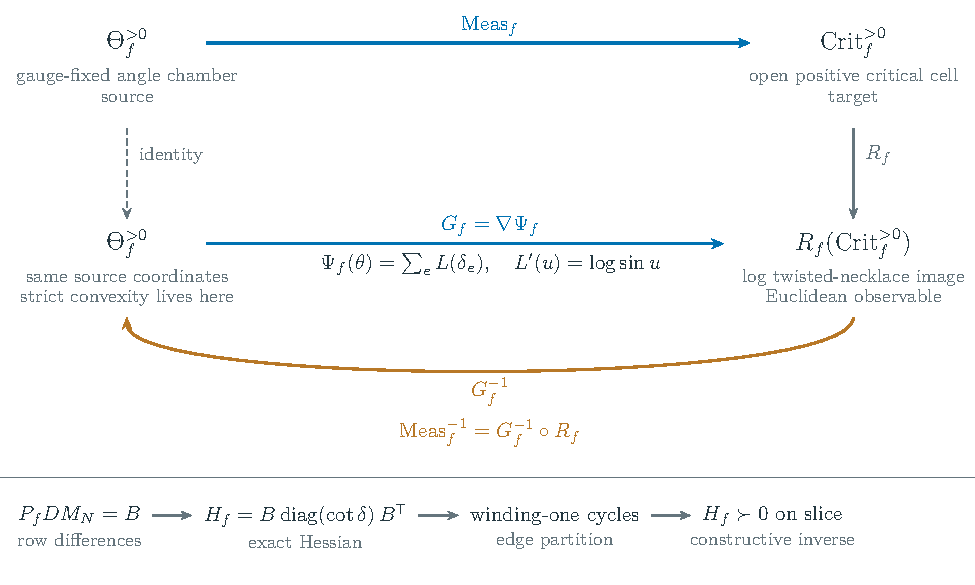
\includegraphics[width=\linewidth]{figures/clh_convex_gradient_inverse.pdf}
\caption{The proof architecture after the Muller--Speyer twist and logarithmic necklace coordinate change. The map becomes the gradient of an explicit potential; the row-difference and winding-cycle identities make its Hessian positive definite on the gauge slice, exposing the constructive inverse.}
\label{fig:clh-architecture}
\end{figure}

\begin{figure}[htbp]
\centering
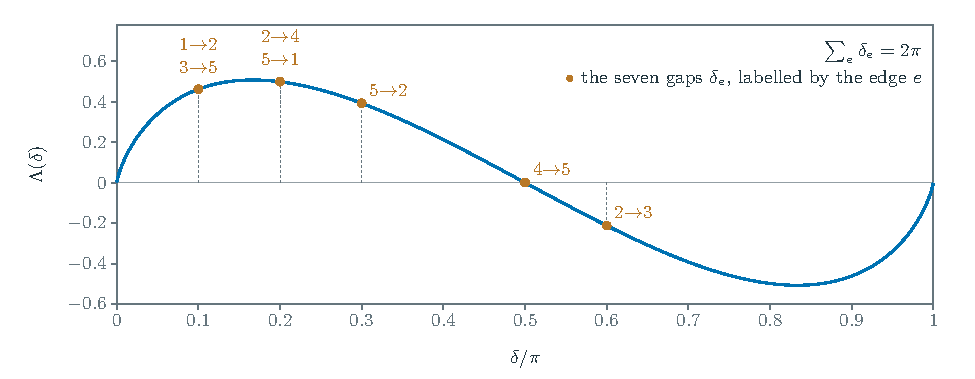
\includegraphics[width=\linewidth]{figures/clh_lean_lobachevsky.pdf}
\caption{The Lobachevsky function $\Lambda(\delta)=-\int_0^{\delta}\log\lvert2\sin t\rvert\,dt$ on $(0,\pi)$, with the seven gaps $\delta_e$ of $\ba=(3,5,1,2,4)$ and $\theta/\pi=(0,0.1,0.7,0.3,0.8)$ marked and labelled by their edges $e$. They sum to $2\pi$, so by \eqref{eq:lobachevsky} $\Psi_f=-\sum_e\Lambda(\delta_e)+\mathrm{const}$. Numerical values, in floating point.}
\label{fig:clh-lean-lobachevsky}
\end{figure}
\section{Setup}\label{sec:setup}

We follow Galashin's conventions \cite[\S1,\S4,\S5]{Galashin}. Let $f$ be loopless of rank $k$ on $[n]$,
with induced permutation $\ba$ and Grassmann necklace $(I_r)_{r\in[n]}$, $I_{r+1}=(I_r\setminus\{r\})\cup\{f(r)\}$.
The \emph{crossing graph} $G_f^{\,x}$ has vertex set all of $[n]$ \cite[eq.~(4.1)]{Galashin}, with an edge
$\{p,q\}$ whenever $p,q$ form an $f$-crossing; we orient it $p\to q$ when the
$\varepsilon$-resolved boundary endpoints occur clockwise as $b^+_{s_p},b^+_{s_q},b^-_p,b^-_q$, where
$s_x=\ba^{-1}(x)$ (\cite[\S5.4]{Galashin}). A label fixed by $\ba$ is an isolated vertex, not an omitted
one. Its connected components partition $[n]$ as $C^{(1)}\sqcup\dots\sqcup C^{(c_f)}$
\cite[\S4.4]{Galashin}; the component-shift
vectors $\{\mathbf 1_C:C\text{ a component}\}$ span the gauge directions, so $\operatorname{rank}B=n-c_f$.

\subsection{The admissibility angles \texorpdfstring{$\delta_e$}{delta e}}\label{sec:delta}

Throughout we use Galashin's affine convention: a tuple $\theta\in\R^n$ is extended to a sequence
indexed by $\Z$ by
\begin{equation}\label{eq:affine-lift}
   \theta_{j+n}=\theta_j+\pi\qquad(j\in\Z)
\end{equation}
\cite[eq.~(3.1)]{Galashin}. For a directed crossing edge $e=(p,q)$ of $G_f^{\,x}$ let $\widetilde q$ be
the \emph{forward lift} of $q$ past $p$, that is $\widetilde q=q$ if $p<q$ and $\widetilde q=q+n$ if
$p>q$, and set
\begin{equation}\label{eq:delta-def}
   \delta_e(\theta):=\theta_{\widetilde q}-\theta_p
   \;=\;\theta_q-\theta_p+\pi\cdot\mathbf 1[p>q].
\end{equation}
An edge with $p>q$ is called \emph{wrapped}. We use the lift to keep the potential
real-valued: the orientation of $G_f^{\,x}$ is given by the endpoint rule above,
so on a wrapped edge the raw difference $\theta_q-\theta_p$ lies in $(-\pi,0)$
and $\log\sin(\theta_q-\theta_p)$ is undefined over $\R$.

With \eqref{eq:delta-def}, admissibility is exactly positivity of the angles:
\begin{equation}\label{eq:adm-delta}
   \theta\in\Theadm
   \iff
   0<\delta_e(\theta)<\pi\ \text{ for every directed crossing edge } e .
\end{equation}
Indeed, \cite[Def.~1.6]{Galashin} imposes $\theta_p<\theta_q<\theta_p+\pi$ for every $f$-crossing $p<q$.
If $e=(p,q)$ with $p<q$ this reads $\delta_e=\theta_q-\theta_p\in(0,\pi)$ directly; if $e=(p,q)$ with
$p>q$, the same inequality applied to the pair $q<p$ gives $\theta_p-\theta_q\in(0,\pi)$, hence
$\delta_e=\pi-(\theta_p-\theta_q)\in(0,\pi)$. In particular $\sin\delta_e>0$ and
$\ell_e:=\log\sin\delta_e$ is defined on all of $\Theadm$.
Figure~\ref{fig:clh-lean-admissible} shows $\Theadm$ on two planes through a point of the worked example of Appendix~\ref{app:worked-example}.
\begin{figure}[htbp]
\centering
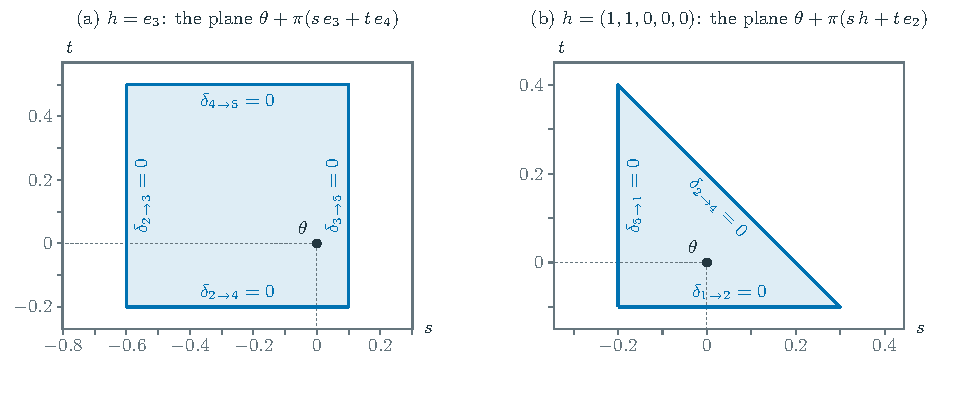
\includegraphics[width=\linewidth]{figures/clh_lean_admissible.pdf}
\caption{The admissible set $\Theadm$ on two planes through $\theta$, for $\ba=(3,5,1,2,4)$ and $\theta/\pi=(0,0.1,0.7,0.3,0.8)$, in the coordinates $(s,t)$ of the point $\theta+\pi(s\,h+t\,v)$. (a) $h=e_3$, $v=e_4$: a rectangle; the plane lies in the affine space of the gauge slice ($h_1=v_1=0$). (b) $h=(1,1,0,0,0)$, $v=e_2$: a triangle. Each side lies on one hyperplane $\delta_e=0$ of \eqref{eq:adm-delta}. Numerical values, in floating point.}
\label{fig:clh-lean-admissible}
\end{figure}

Two consequences of \eqref{eq:delta-def} are used repeatedly. First, the oriented increment is
unaffected by the lift,
\begin{equation}\label{eq:delta-increment}
   \partial_\theta\delta_e=e_q-e_p ,
\end{equation}
so $\delta_e$ is an \emph{affine} (not linear) function of $\theta$, constant along component shifts.
Second, passing from $\theta_q$ to its lift $\theta_q+\pi$ leaves $\lvert\sin\delta_e\rvert$ and
$\cot\delta_e$ unchanged but \emph{reverses the sign} of $\sin\delta_e$; the quantity the potential needs
is $\sin\delta_e>0$, and that is what \eqref{eq:adm-delta} delivers.
With the edge orientations, and hence $B$, fixed, writing
$\ell_e=\log\lvert\sin(\theta_q-\theta_p)\rvert$ gives the same gradient values;
the $\pi$-periodicity of cotangent likewise leaves the Hessian unchanged.
The lift supplies the real domain of $L'=\log\sin$ and the positive cycle
angles whose sum is $\pi$, as used in the convexity argument below. This
invariance under adding $\pi$ does not authorize changing edge orientations.
Figure~\ref{fig:clh-lean-gauge} shows two shifts of $\theta$ on the worked example: one constant on the crossing component, which changes no $\delta_e$, and one that is not.
\begin{figure}[htbp]
\centering
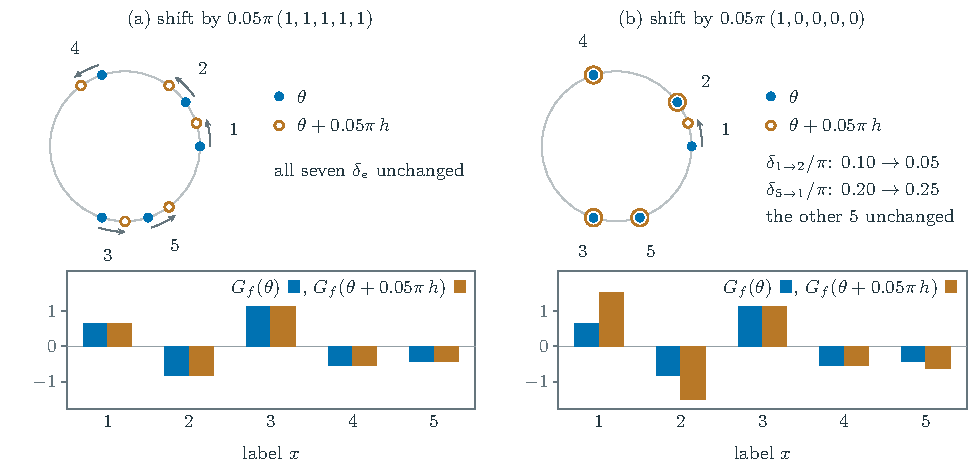
\includegraphics[width=\linewidth]{figures/clh_lean_gauge.pdf}
\caption{The shift $\theta\mapsto\theta+0.05\pi\,h$ for $\ba=(3,5,1,2,4)$ and $\theta/\pi=(0,0.1,0.7,0.3,0.8)$. Points are $e^{2i\theta_p}$ before (filled) and after (open); bars give $G_f=B\ell$ at each label. (a) $h=(1,1,1,1,1)$, constant on the crossing component: every $\delta_e$ and $G_f$ are unchanged. (b) $h=e_1$, which moves $\theta_1$ alone: $\delta_{1\to2}$ and $\delta_{5\to1}$ change, and $G_f$ with them. Numerical values, in floating point.}
\label{fig:clh-lean-gauge}
\end{figure}

Finally we record the cycle identity that Lemma~\ref{lem:cot} will consume. A directed cycle
$Z=(p_1\to p_2\to\cdots\to p_m\to p_1)$ of crossing edges has winding one --- total exit-advance $n$ ---
if and only if it has exactly one descent in the cyclic label order, i.e.\ exactly one wrapped edge (see
the closing paragraph of \S\ref{sec:wp-combinatorial-bridge} --- a forward reference; nothing in
\S\ref{sec:wp-combinatorial-bridge} depends on this section, so there is no circularity). Lifting each
successive exit forward, the
sum of \eqref{eq:delta-def} along $Z$ telescopes to $\theta_{p_1+n}-\theta_{p_1}$, so by
\eqref{eq:affine-lift}
\begin{equation}\label{eq:cycle-sum}
   \sum_{e\in Z}\delta_e(\theta)=\pi
   \qquad\text{for every winding-one cycle }Z\text{ and every }\theta .
\end{equation}
This is an identity in $\theta$ on all of $\R^n$, not a constraint cutting out $\Theadm$.

\subsection{Galashin's complex parameters, the bracket, and the hinge identity}\label{sec:bracket}

The exponent formula we import is stated in the complex parameters of \cite[\S1.4]{Galashin}, so we fix
that notation here rather than inside the proof that uses it. Let $\mathcal G_{\mathrm{red}}(f)$ be the
set of reduced planar bipartite graphs in the disk with strand permutation $\ba$, and for a weight
function $\mathrm{wt}$ on $E(G)$ let $\Meas_G(\mathrm{wt}):=(\Delta_I(G,\mathrm{wt}))_{I\in\binom{[n]}k}$
be the vector of dimer partition functions, viewed in $\Gr(k,n)$ when it is nonzero
\cite[\S1.1,\S5.1]{Galashin}. Let $\widetilde\tau$ denote the Muller--Speyer \emph{left twist}
automorphism of the open positroid variety $\Pi_f^\circ$ (\cite[\S5.4, eq.~(5.6)]{Galashin},
\cite{MullerSpeyer}).

For $x,y\in\C^*$ put
\begin{equation}\label{eq:bracket}
   [\![x,y]\!]:=\frac xy-\frac yx ,
\end{equation}
and for $t=(t_1,\dots,t_n)\in(\C^*)^n$ let $\mathrm{wt}_t$ be the weight function which gives an interior
edge labelled $\{p,q\}$, $p<q$, the weight $[\![t_q,t_p]\!]$ and every boundary edge the weight $1$
\cite[Def.~1.12, eq.~(1.4)]{Galashin}. Following \cite[\S5.4]{Galashin} we abbreviate
\begin{equation}\label{eq:bracket-plus}
   [\![t_p,t_q]\!]_+=[\![t_q,t_p]\!]_+:=[\![t_q,t_p]\!]\qquad(1\le p<q\le n),
\end{equation}
which is the symmetric form in which the brackets appear in \eqref{eq:gal512}. The tuple $t$ is
$f$-admissible when $t_p\ne\pm t_q$ for every $f$-crossing $\{p,q\}$, and
\begin{equation}\label{eq:theta-circ}
   \Theta_f^{\circ}:=\{t\in(\C^*)^n:\ t\ \text{is }f\text{-admissible and }
   t_{p_1}=\cdots=t_{p_{c_f}}=1\}
\end{equation}
\cite[eq.~(5.2)]{Galashin} is the complex analogue of the gauge slice $\Thef$, with $p_1,\dots,p_{c_f}$
the same component representatives that cut out $\Thef$ in \cite[eq.~(4.3)]{Galashin}.

Angles enter through the specialization of \cite[eq.~(5.1)]{Galashin},
\begin{equation}\label{eq:t-of-theta}
   t_p:=\exp(i\theta_p)\qquad(p\in[n]),
\end{equation}
under which $\mathrm{wt}_\theta=\tfrac1{2i}\,\mathrm{wt}_t$ on interior edges. The two weight functions
are gauge-equivalent, so \cite[Lem.~5.13]{Galashin} gives, for every $G\in\mathcal G_{\mathrm{red}}(f)$
and every $f$-admissible $\theta$,
\begin{equation}\label{eq:meas-identification}
   \Meas_G(\mathrm{wt}_t)=\Meas_G(\mathrm{wt}_\theta)=\Meas_f(\theta)\quad\text{in }\Gr(k,n),
\end{equation}
the last equality being the square-move invariance by which $\Meas_f(\theta)$ is defined
\cite[\S1.2]{Galashin}. Thus \eqref{eq:gal512} below, although written in $t$, is a statement about
$\Meas_f(\theta)$.

\begin{lemma}[Hinge identity]\label{lem:hinge}
Under \eqref{eq:t-of-theta}, for every directed crossing edge $e=(p,q)$ and every $\theta\in\Theadm$,
\begin{equation}\label{eq:hinge}
   \bigl\lvert[\![t_q,t_p]\!]_+\bigr\rvert=2\sin\delta_e(\theta).
\end{equation}
\end{lemma}

\begin{proof}
By \eqref{eq:bracket} and \eqref{eq:t-of-theta}, for any $a,b\in[n]$,
$[\![t_a,t_b]\!]=e^{i(\theta_a-\theta_b)}-e^{-i(\theta_a-\theta_b)}=2i\sin(\theta_a-\theta_b)$, so
$\lvert[\![t_a,t_b]\!]\rvert=2\lvert\sin(\theta_a-\theta_b)\rvert$. Both orientations of the edge are now
covered. If $p<q$, \eqref{eq:bracket-plus} gives $[\![t_q,t_p]\!]_+=[\![t_q,t_p]\!]$ and
$\delta_e=\theta_q-\theta_p\in(0,\pi)$, so both sides equal $2\sin(\theta_q-\theta_p)$. If $p>q$ --- the
wrapped case --- then $[\![t_q,t_p]\!]_+=[\![t_p,t_q]\!]$ because $q<p$, whose modulus is
$2\lvert\sin(\theta_p-\theta_q)\rvert=2\sin(\theta_p-\theta_q)$ by admissibility, while
$\delta_e=\pi-(\theta_p-\theta_q)$ gives $\sin\delta_e=\sin(\theta_p-\theta_q)$. The two sides agree
again.
\end{proof}

\begin{remark}[the hinge is a chord length]\label{rem:chord}
Setting $v_r:=\exp(2i\theta_r)$, Galashin observes that $\sin(\theta_q-\theta_p)=\tfrac12\lvert
v_q-v_p\rvert$ \cite[Rem.~1.2]{Galashin}. So \eqref{eq:hinge} says that the edge factor of a crossing is
the distance between two points $v_p,v_q$ on a circle, and the argument of the sine is pinned by that
reading: $\lvert[\![t_q,t_p]\!]_+\rvert=\lvert v_q-v_p\rvert$, not $c\sin(\delta_e/2)$ or
$c\sin(2\delta_e)$. For $k=3$, $n=4$, \cite[Ex.~1.9]{Galashin} reads the resulting Pl\"ucker coordinates
as the side lengths of a convex inscribed quadrilateral. Admissibility does not put all $n$ points in
cyclic order: for $f=(3,5,6,7,9)$ and $\theta/\pi=(0,0.1,0.7,0.3,0.8)$, the worked example of
Appendix~\ref{app:worked-example}, every crossing angle lies in $(0,\pi)$,
yet labels $3$ and $4$ are out of order. The vertices of each winding-one cycle are in cyclic order, since
their angles $2\delta_e$ are positive and sum to $2\pi$; that is all the volume reading of
\S\ref{sec:intro} uses.
\end{remark}

Figure~\ref{fig:clh-lean-hinge} draws the points $v_r$ and the chords $\lvert v_q-v_p\rvert$ for the worked example of Appendix~\ref{app:worked-example}.

\begin{figure}[htbp]
\centering
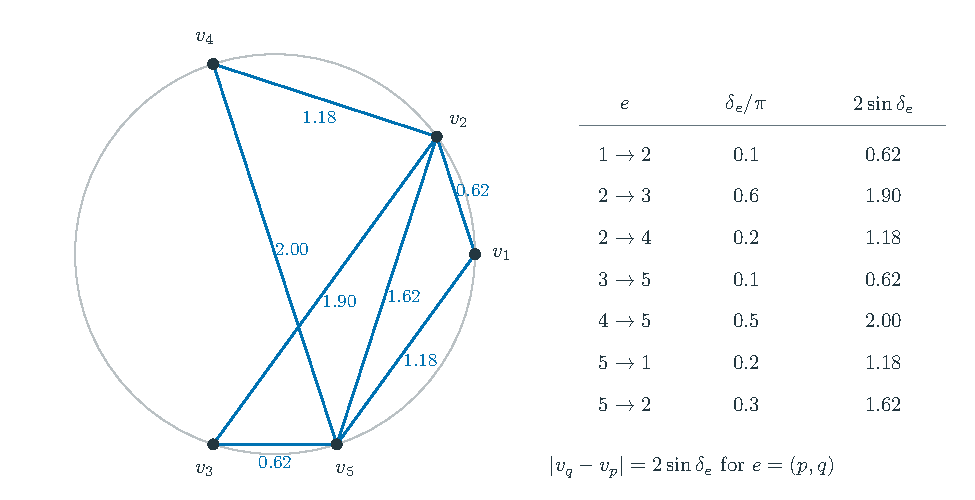
\includegraphics[width=\linewidth]{figures/clh_lean_hinge.pdf}
\caption{The points $v_r=e^{2i\theta_r}$ on the unit circle for $f=(3,5,6,7,9)$ and $\theta/\pi=(0,0.1,0.7,0.3,0.8)$. Each directed crossing edge $e=(p,q)$ is the chord from $v_p$ to $v_q$, labelled by its length $\lvert v_q-v_p\rvert=2\sin\delta_e$ as in \eqref{eq:hinge}; the table lists $\delta_e/\pi$ and $2\sin\delta_e$. Numerical values, in floating point.}
\label{fig:clh-lean-hinge}
\end{figure}

\subsection{The necklace exponent matrix}\label{sec:mn}

The \emph{necklace exponent matrix} $M_N$ has rows indexed by the necklace positions
$r\in[n]$ and columns by unordered pairs $\{p,q\}$; by Galashin's Proposition~5.12 (eq.~(5.8), displayed
as \eqref{eq:gal512} below) the twisted
Pl\"ucker coordinate $\Delta_{I_r}(\widetilde\tau(\cdot))$ is a monomial whose $\{p,q\}$-exponent is determined by the
pair's misalignment/crossing class together with the membership of $p,q$ in $I_r$. We index $B$ by the
same set of unordered pairs: since the crossing relation is antisymmetric (again the closing paragraph of
\S\ref{sec:wp-combinatorial-bridge}, a forward reference of the same harmless kind), a pair $\{p,q\}$
carries at
most one directed crossing edge, and we let its $B$-column be $e_q-e_p$ when $p\to q$ is that edge and
the zero column when $\{p,q\}$ carries no crossing. With this convention $M_N$ and $B$ have the same
column set, the vector $\ell=(\ell_e)$ is understood as extended by an arbitrary value on non-crossing
pairs, and every such value is annihilated by the corresponding zero column of $B$. All identities below
are proved column by column, so the extension is immaterial.

\subsection{Coloops, and the component reduction}\label{sec:reduction}

A label fixed by $\ba$ --- a coloop, $f(p)=p+n$ --- is an isolated vertex of $G_f^{\,x}$ and carries no
crossing (proved in the ``Coloops'' step of Proposition~\ref{prop:rowdiff}), so it contributes nothing to
$\Psi_f$, to $B$, or to $H_f$. The fixed-point-free case is
therefore the essential one. Two independent devices make this precise, and we record both because they
discharge different worries: Proposition~\ref{prop:rowdiff} is proved below \emph{with coloops allowed},
so no statement in this paper carries a fixed-point-free hypothesis; and the component reduction of this
subsection independently factors the whole problem over the components of $G_f^{\,x}$.

\begin{lemma}[Component reduction]\label{lem:reduction}
Let $f$ be loopless and let $[n]=C^{(1)}\sqcup\dots\sqcup C^{(c_f)}$ be the connected components of
$G_f^{\,x}$. Then:
\begin{enumerate}
\item for each $r$, erasing from the strand diagram $D_f$ every strand $S_p$ with $p\notin C^{(r)}$ and
relabeling the surviving strands and boundary vertices by $[n_r]$, $n_r=|C^{(r)}|$, yields a strand diagram
in the sense of \cite[Def.~4.5]{Galashin}; its strand permutation is a loopless bounded affine permutation
$f^{(r)}:=f|_{C^{(r)}}\in\mathcal B(k_r,n_r)$ \textup{\cite[\S4.4]{Galashin}};
\item the restriction map $\rho:\theta\mapsto(\theta|_{C^{(1)}},\dots,\theta|_{C^{(c_f)}})$ is a
homeomorphism $\Thef\to\Theta_{f^{(1)}}^{>0}\times\cdots\times\Theta_{f^{(c_f)}}^{>0}$, and there is a
homeomorphism $\Sigma:\Critf\xrightarrow{\ \sim\ }
\Crit_{f^{(1)}}^{>0}\times\cdots\times\Crit_{f^{(c_f)}}^{>0}$
\textup{\cite[Prop.~4.10]{Galashin}} which \emph{intertwines the measurement maps}: the square
\begin{equation}\label{eq:reduction-square}
\begin{array}{ccc}
 \Thef & \xrightarrow{\ \rho\ } & \prod_r\Theta_{f^{(r)}}^{>0}\\[2pt]
 \ \downarrow{\scriptstyle\Meas_f} & &\ \downarrow{\scriptstyle\prod_r\Meas_{f^{(r)}}}\\[2pt]
 \Critf & \xrightarrow{\ \Sigma\ } & \prod_r\Crit_{f^{(r)}}^{>0}
\end{array}
\end{equation}
commutes, i.e.\ $\Sigma(\Meas_f(\theta))=\bigl(\Meas_{f^{(r)}}(\theta|_{C^{(r)}})\bigr)_r$;
\item if $C^{(r)}=\{p\}$ is a singleton then $S_p$ crosses nothing, $\Theta_{f^{(r)}}^{>0}$ is a point, and
the factor is a point;
\item every non-singleton $C^{(r)}$ has $\overline{f^{(r)}}$ fixed-point-free.
\end{enumerate}
\end{lemma}

\begin{proof}
Part~(1) is \cite[\S4.4]{Galashin}: after the erasure the directions of the surviving strands
still alternate around the boundary of the disk, so the relabeled diagram is a strand diagram in the
sense of \cite[Def.~4.5]{Galashin}.

For~(2), the commutation in \eqref{eq:reduction-square} is not an extra hypothesis: it is how
Proposition~4.10 of \cite{Galashin} is proved. There the disk is split at a boundary label whose two
$\varepsilon$-resolved endpoints lie in different components, producing two cyclic intervals $P,Q$, each
a union of components of $G_f^{\,x}$, with restrictions $g=f|_P$ and $h=f|_Q$. Galashin first records
that $\theta$ is $f$-admissible if and only if $\theta|_P$ is $g$-admissible and $\theta|_Q$ is
$h$-admissible, and then establishes the homeomorphism by the explicit minor identities (4.4)--(4.6)
between $X=\Meas_f(\theta)$ and the pair $\bigl(\Meas_g(\theta|_P),\Meas_h(\theta|_Q)\bigr)$, showing
that each determines the other. In other words the map exhibited there is
$\Meas_f(\theta)\mapsto\bigl(\Meas_g(\theta|_P),\Meas_h(\theta|_Q)\bigr)$, which is exactly the
commuting square for a two-factor splitting; iterating the splitting over the $c_f$ components gives
\eqref{eq:reduction-square}. The top arrow $\rho$ is a homeomorphism because admissibility is a
conjunction of conditions each involving a single component (both labels of an $f$-crossing lie in one
component), and because the gauge slice fixes exactly one angle in each component, so $\rho$ is the
restriction of a linear isomorphism between the ambient affine slices.

For~(3), an isolated vertex of $G_f^{\,x}$ is a strand
crossing no other, so the erased diagram has a single strand and no admissibility constraint; the gauge
fixes its angle. For~(4), a fixed point of $\overline{f^{(r)}}$ is a strand of $D_f|_{C^{(r)}}$ running
between adjacent $\varepsilon$-resolved endpoints, which therefore crosses no other surviving strand and is
isolated in the crossing graph of $f^{(r)}$; since that graph is connected and $n_r\ge2$, there is no such
strand.
\end{proof}

\begin{remark}[why this is not a restriction of $\ba$]\label{rem:not-restriction}
Part~(1) is an erasure-and-relabeling, not the restriction of $\ba$ to an invariant subset, and the
distinction is not cosmetic: a component of $G_f^{\,x}$ need not be $\ba$-stable. Galashin flags the
mechanism --- for $p\in[n]$ the endpoints $b^-_p$ and $b^+_p$ may lie in different components of $D_f$,
so the boundary vertex $b_p$ appears to belong to two components at once \cite[\S4.4]{Galashin}. The
smallest instance is $n=2$, $\ba=(2\,1)$: both chords join adjacent $\varepsilon$-resolved endpoints, so
$G_f^{\,x}$ has no edges and $\{1\}$ is a component, yet $\ba(1)=2$. Relabeling after erasure is what makes
$f^{(r)}$ well defined regardless.
\end{remark}

Because \eqref{eq:reduction-square} commutes and its horizontal arrows are homeomorphisms, $\Meas_f$ is a
homeomorphism $\Thef\to\Critf$ if and only if every $\Meas_{f^{(r)}}$ is one on its factor; and a finite
product of homeomorphisms is a homeomorphism. So Theorem~\ref{thm:main} for all loopless $f$ follows from
Theorem~\ref{thm:main} for those $f$ with $\ba$ fixed-point-free.

\begin{remark}[no standing fixed-point-free hypothesis]\label{rem:no-fpf}
The proof of Proposition~\ref{prop:rowdiff} covers coloops directly (the ``Coloops'' step below), and
Proposition~\ref{prop:wp}, Proposition~\ref{prop:psd} and Theorem~\ref{thm:main} are stated and proved
for every loopless $f$. No statement in \S\ref{sec:gradient}--\S\ref{sec:shift} assumes $\ba$
fixed-point-free. Lemma~\ref{lem:reduction} is therefore not needed for the general loopless case; we
keep it because it identifies the product structure of $\Critf$ and gives a second, independent route to
it.
\end{remark}

\begin{remark}[loops: a proof candidate for the extension, not claimed here]\label{rem:loops}
Galashin states Conjecture~4.3 for loopless $f$ only, and Theorem~\ref{thm:main} is stated on exactly that
domain. Reading \cite[Def.~1.8]{Galashin} verbatim for an arbitrary $f\in\mathcal B(k,n)$ --- a reading
that is ours, not Galashin's, since his Section~4 fixes $f$ loopless --- a loop label $p$ (that is,
$f(p)=p$) is a lollipop in every reduced graph \cite[\S2.2]{Galashin}: its boundary vertex is white and
adjacent to a black interior leaf, so the pendant edge lies in every almost perfect matching, carries
weight $1$, and forces $p$ out of the index set of every nonvanishing minor. Hence the $p$-th column
of $\Meas_f(\theta)$ vanishes, $p$ is an isolated vertex of $G_f^{\,x}$, $\Theadm=\Theta_{f'}^{\mathrm{adm}}\times\R$,
and deleting the lollipop leaves a graph with strand permutation $f'=f\setminus\{p\}$,
a bounded affine permutation of period $n-1$ and rank $k$. That graph is again reduced: deleting a pendant
edge with a free end keeps the $k(n-k)+1-\ell(f)$ faces of a reduced graph \cite[\S2.2]{Galashin},
and $\ell(f)=\ell(f')+k$ (stated in the proof of \cite[Thm.~7.12]{LamGrassmann}) makes this the count
$k(n-1-k)+1-\ell(f')$ that characterizes the reduced graphs for $f'$; independently, the four conditions
of \cite[Thm.~13.2]{Postnikov} pass to the deleted graph, the lollipop's edge lying on no other trip.
The combinatorial facts are Lean theorems (\texttt{TP.\allowbreak deleteLoop\_\allowbreak bdd}, \texttt{TP.\allowbreak affRank\_\allowbreak deleteLoop}, \texttt{TP.\allowbreak affLength\_\allowbreak deleteLoop}). So $\Meas_f(\theta)$ is the image of
$\Meas_{f'}(\theta')$, $\theta'$ the other angles, under the zero-column embedding $\Gr(k,n-1)\hookrightarrow\Gr(k,n)$,
and the looped statement, that $\Meas_f$ is a homeomorphism from the gauge slice onto
$\Critf$, follows from Theorem~\ref{thm:main} for $f$ with its loops deleted. This is a proof candidate
under the reading above; \emph{none of it is claimed in this paper}, whose scope remains loopless.
\end{remark}

Figure~\ref{fig:clh-lean-reduction} shows the two constructions of this subsection: the components of the crossing graph (Lemma~\ref{lem:reduction}) and the deletion of a loop (Remark~\ref{rem:loops}).

\begin{figure}[htbp]
\centering
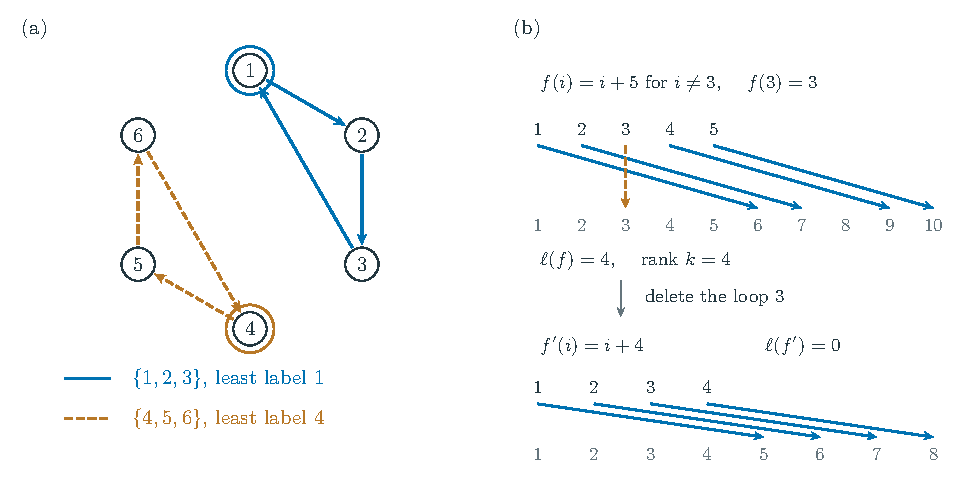
\includegraphics[width=\linewidth]{figures/clh_lean_reduction.pdf}
\caption{(a) The crossing graph of the loopless $f$ with $\ba=(3,1,2,6,4,5)$ has two connected components, $\{1,2,3\}$ (blue, solid) and $\{4,5,6\}$ (ochre, dashed); the ringed vertex is the least label of its component. (b) Deleting a loop: $n=5$, $f(i)=i+5$ except $f(3)=3$; here $\ell(f)=4$ and $k=4$, and after the deletion $\ell(f')=0$. Panel (a) is evaluated by the formal definitions of Appendix~\ref{app:lean-interface}; the lengths and the rank in panel (b) are counted directly.}
\label{fig:clh-lean-reduction}
\end{figure}

\section{The measurement map is a gradient}\label{sec:gradient}

\subsection{The row-difference identity}
The engine of \eqref{eq:gradient} is an exact integer-matrix identity between Galashin's necklace exponents
and the crossing incidence. Let $D$ be the cyclic forward row-difference $(Dz)_r=z_{r+1}-z_r$ and let
$P_f$ be the necklace relabeling $(P_fz)_x=z_{s_x}$.

The proof of that identity rests on one bookkeeping fact about the $\varepsilon$-resolved boundary,
which we isolate first. Split each boundary position $j\in[n]$ into an exit point $j^-$ followed clockwise by an entry
point $j^+$, Galashin's $b^-_j$ and $b^+_j$ \cite[Def.~1.5]{Galashin}, so that the $2n$ refined points
occur clockwise as $1^-,1^+,2^-,2^+,\dots,n^-,n^+$. For an entry point $u^+$ and an exit point $v^-$,
let $J(u^+,v^-)$ be the set of refined points met when moving clockwise from $u^+$, excluding $u^+$
and including $v^-$. For $u,v\in[n]$ write $(u,v]$ for the cyclic half-open integer arc
$\{u+1,u+2,\dots,v\}$, indices modulo $n$, with $(u,u]:=[n]$.

\begin{lemma}[Half-open reading of the resolved boundary]\label{lem:halfopen}
\leavevmode
\begin{enumerate}
\item[\textup{(a)}] For all $u,v\in[n]$, $\{r\in[n]:r^-\in J(u^+,v^-)\}=(u,v]$.
\item[\textup{(b)}] If $j^-$ and $j^+$ both occur in a list of distinct refined points written in
clockwise cyclic order, then $j^+$ immediately follows $j^-$ in that list.
\item[\textup{(c)}] Let $a^+,c^+$ be entry points and $b^-,d^-$ exit points, the four refined points
being distinct. Then
\begin{align}
   a^+,b^-,c^+,d^-\ \text{clockwise} &\ \Longrightarrow\ (a,b]\cap(c,d]=\varnothing;\label{eq:L1}\\
   a^+,b^-,c^+,d^-\ \text{counterclockwise} &\ \Longrightarrow\ (a,b]\cup(c,d]=[n];\label{eq:L2}\\
   a^+,c^+,b^-,d^-\ \text{clockwise} &\ \Longrightarrow\ (a,b]\setminus(c,d]=(a,c].\label{eq:L3}
\end{align}
\end{enumerate}
\end{lemma}

\begin{proof}
(a) Moving clockwise from $u^+$ one meets $(u+1)^-,(u+1)^+,(u+2)^-,\dots$, so the exit points in
$J(u^+,v^-)$ are the $r^-$ with $r=u+1,u+2,\dots,v$, read modulo $n$. If $u=v$, the walk reaches
$u^-$, the last refined point before $u^+$, only after every other exit point.

(b) No refined point lies strictly between $j^-$ and $j^+$ on the clockwise circle, so in any cyclic
list containing both, the successor of $j^-$ is $j^+$.

(c) Write the four points in clockwise order, compare refined arcs, and read rows with (a). In
\eqref{eq:L1} the arcs $J(a^+,b^-)$ and $J(c^+,d^-)$ are the clockwise stretches from $a^+$ to $b^-$
and from $c^+$ to $d^-$ of the order $a^+,b^-,c^+,d^-$; they are disjoint, so no exit point lies in
both. In \eqref{eq:L2} the clockwise order is $a^+,d^-,c^+,b^-$, and the complements of the two arcs
are the stretches from $b^-$ to $a^+$ and from $d^-$ to $c^+$ (each without its first point and with
its last), which are disjoint; so every exit point lies in $J(a^+,b^-)$ or in $J(c^+,d^-)$. In
\eqref{eq:L3} the clockwise order is $a^+,c^+,b^-,d^-$, and $J(a^+,b^-)\setminus J(c^+,d^-)$ is the
stretch from $a^+$ (excluded) to $c^+$ (included). Its exit points are those of $J(a^+,c^-)$, because
$c^-$ is the refined point just before $c^+$ and is not $a^+$; by (a) they are the rows of $(a,c]$.
\end{proof}

Part (b) is the exit-before-entry rule at a shared label, and it decides which integer coincidences
the three patterns of (c) admit. Two of the four points can share an integer only if one is an exit
and the other an entry, and then only where, in the pattern, that exit is immediately followed by
that entry. In \eqref{eq:L1} this allows $b=c$ and $d=a$; in \eqref{eq:L2}, whose clockwise order is
$a^+,d^-,c^+,b^-$, only $c=d$ and $a=b$; in \eqref{eq:L3} only $d=a$, while $c=b$ is excluded because
$c^+$ would be followed by $c^-$. Part (c) needs no other case distinction: it assumes only that the
four refined points are distinct. Figure~\ref{fig:clh-halfopen} draws the reading (a) and the three
patterns, each with a shared label where one is allowed.

\begin{figure}[t]
\centering
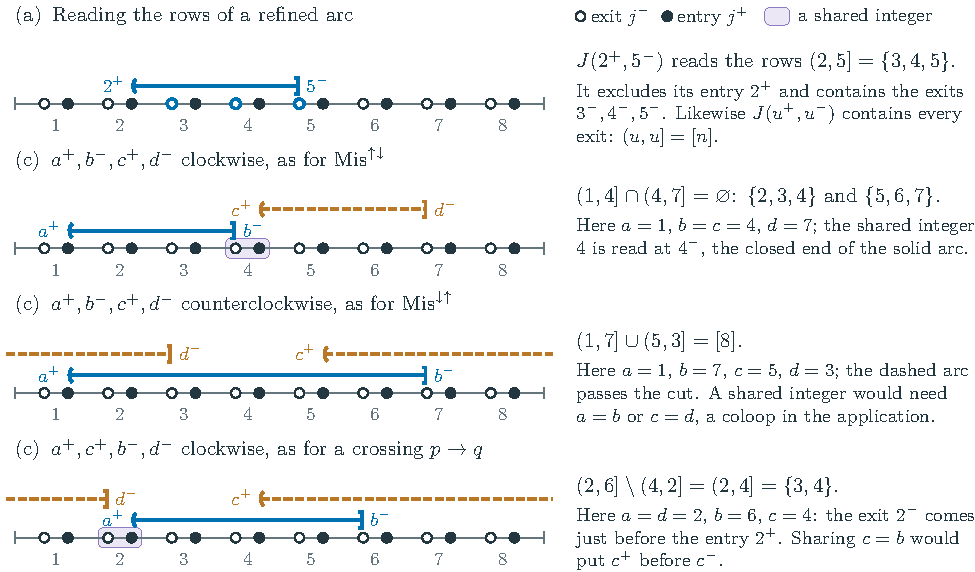
\includegraphics[width=\linewidth]{figures/clh_halfopen_arcs.pdf}
\caption{Lemma~\ref{lem:halfopen} on the resolved boundary, cut open for $n=8$; open points are exits $j^-$ and filled points entries $j^+$. A row $r$ is read at its exit point $r^-$, so the refined arc $J(u^+,v^-)$, drawn from its open end $u^+$ to its closed end $v^-$, reads the half-open arc $(u,v]$. In part (c), with $(a,b,c,d)=(s_p,p,s_q,q)$ as in the proof of Proposition~\ref{prop:rowdiff}, the solid arc $J(a^+,b^-)$ reads $A_p$ and the dashed arc $J(c^+,d^-)$ reads $A_q$. In the first and third patterns an integer is shared, and its exit comes immediately before its entry. Schematic; the positions are illustrative.}
\label{fig:clh-halfopen}
\end{figure}

\begin{proposition}\label{prop:rowdiff}
For every loopless $f$,
\[
   P_f\,D\,M_N \;=\; B,
\]
where $M_N$ is the necklace-row restriction of Galashin's Proposition~5.12 exponent matrix and $B$ is the
directed incidence matrix of $G_f^{\,x}$, both indexed by unordered pairs as in \S\ref{sec:mn}.
\end{proposition}

\begin{figure}[htbp]
\centering
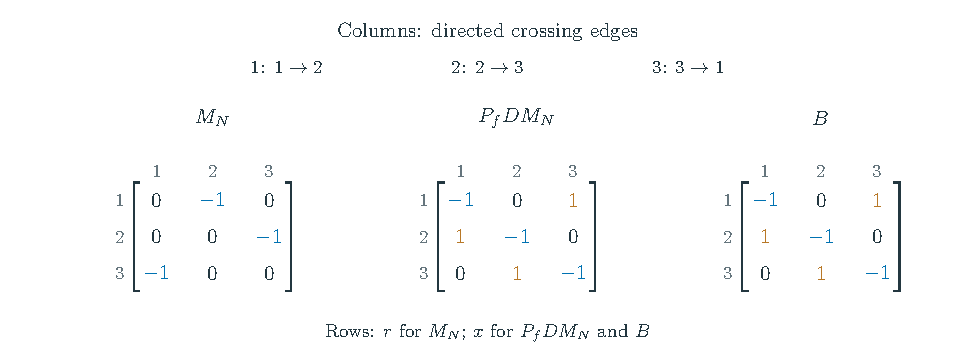
\includegraphics[width=\linewidth]{figures/clh_matrix_small.pdf}
\caption{The row-difference identity for $\ba=(3,1,2)$. The columns are the three crossings $1\to2$, $2\to3$, $3\to1$, each with $s_p=q$. Rows of $M_N$ are necklace positions; rows of $P_fDM_N$ and $B$ are exit labels. Thus the negative arc indicators become incidence columns, with $-1$ at the tail and $+1$ at the head.}
\label{fig:clh-matrix-small}
\end{figure}

\begin{proof}
The identity is the boundary of a half-open arc, read column by column. We show below that the columns of
$M_N$ are as follows: a pair carrying no directed crossing, in either direction, has a zero column, which
covers every pair meeting a coloop; and for a crossing $p\to q$ the column is
\[
   m_r=-\mathbf 1_{r\in(s_p,s_q]},
\]
minus the indicator of the cyclic half-open arc of rows from $s_p$ to $s_q$. Granting this, a pair carrying no
crossing has a zero column in $P_fDM_N$ and in $B$, which is the incidence matrix of the crossings. For a
crossing $p\to q$ the indicator of $(s_p,s_q]$ changes only from row $s_p$ to $s_p+1$, where it enters the
arc, and from row $s_q$ to $s_q+1$, where it leaves (these differ, $\ba$ being injective), so
\[
   (Dm)_r=m_{r+1}-m_r=\mathbf 1_{r=s_q}-\mathbf 1_{r=s_p},\qquad Dm=e_{s_q}-e_{s_p},
\]
and relabeling by $P_f$ gives $P_fDm=e_q-e_p$, the incidence column $B_{p\to q}$. Hence $P_fDM_N=B$. It
remains to compute the columns.

\emph{The columns of $M_N$.}
By Galashin's affine formula $I_r=\{f(a)\bmod n : a<r\le f(a)\}$, a label $x$ lies in $I_r$ iff, for the
lift $s$ of $s_x$ with the paired lift $x'$ of $x$ obeying $0<x'-s\le n$, one has $s<r\le x'$. Reducing
modulo $n$,
\begin{equation}\label{eq:arc}
   x\in I_r \iff r\in A_x:=(s_x,x]\ \text{(cyclically)}.
\end{equation}
The inequality $x'-s\le n$ is strict exactly when $x$ is not a coloop; for a coloop ($\ba(x)=x$, so
$s_x=x$ and $f(x)=x+n$) one has $x'-s=n$, and $A_x$ is then the whole row set $[n]$ --- $x$ lies in
\emph{every} necklace row. Both readings are used below. In the language of
Lemma~\ref{lem:halfopen}(a), $A_x$ is read off the refined arc $J(s_x^+,x^-)$ swept by the strand $S_x$,
and the three half-open arc facts \eqref{eq:L1}--\eqref{eq:L3} are that lemma's part (c). They hold for
the $\varepsilon$-resolved order with no generic-position assumption, because the four refined
endpoints of two distinct labels are always distinct.

We now recall the exponent formula itself, since the argument turns on exactly which pairs contribute and
with which sign. For $p\ne q$ write $s=s_p$ and $t=s_q$; following \cite[\S5.4]{Galashin}, one says
$\{p,q\}\in\mathrm{Mis}^{\uparrow\downarrow}_f$ when $b^+_{s},b^-_p,b^+_{t},b^-_q$ occur clockwise, and
$\{p,q\}\in\mathrm{Mis}^{\downarrow\uparrow}_f$ when they occur counterclockwise; the two-element sets
$\{s,t\}$ and $\{p,q\}$ are not required to be disjoint, so these definitions explicitly admit
coincidences. Figure~\ref{fig:clh-pair-classes} illustrates these classes together with a crossing and an alignment.

\begin{figure}[htbp]
\centering
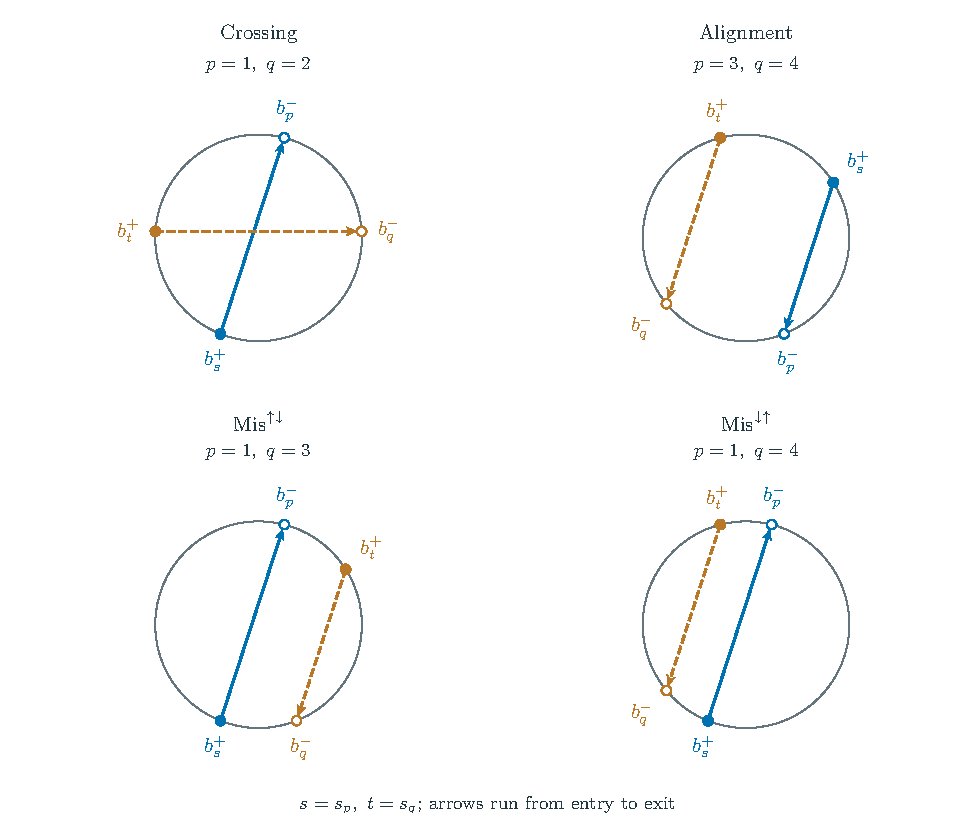
\includegraphics[width=\linewidth]{figures/clh_pair_classes.pdf}
\caption{The four pair classes for $\ba=(3,5,1,2,4)$, with $s=s_p$ and $t=s_q$. Each circle is read clockwise. The blue solid strand runs from $b_s^+$ to $b_p^-$; the ochre dashed strand runs from $b_t^+$ to $b_q^-$. Filled points are entries and open points are exits. The crossing has order $b_s^+,b_t^+,b_p^-,b_q^-$; the alignment has order $b_s^+,b_p^-,b_q^-,b_t^+$. The two misalignments read $b_s^+,b_p^-,b_t^+,b_q^-$ clockwise and counterclockwise, respectively.}
\label{fig:clh-pair-classes}
\end{figure}

With $[\![t_p,t_q]\!]_+=[\![t_q,t_p]\!]_+:=[\![t_q,t_p]\!]$ for $p<q$, Proposition~5.12 of
\cite{Galashin} states that, for $G\in\mathcal G_{\mathrm{red}}(f)$ and $t\in\Theta_f^{\circ}$ at which
$\Meas_G$ is defined, after multiplication by a common scalar
\begin{equation}\label{eq:gal512}
 \Delta_I\bigl(\widetilde\tau(\Meas_G(\mathrm{wt}_t))\bigr)
 =\!\!\prod_{\substack{\{p,q\}\in\mathrm{Mis}^{\uparrow\downarrow}_f\\ p,q\in I}}\!\!
   [\![t_q,t_p]\!]_+
 \cdot\!\!\prod_{\substack{\{p,q\}\in\mathrm{Mis}^{\downarrow\uparrow}_f\\ p,q\notin I}}\!\!
   [\![t_q,t_p]\!]_+
 \cdot\Biggl(\ \prod_{\substack{(p,q)\in E(\vec G^{\,\times}_f)\\ p\in I,\ q\notin I}}\!\!
   [\![t_q,t_p]\!]_+\Biggr)^{\!-1}
\end{equation}
for every face label $I$ of $G$ \cite[eq.~(5.8)]{Galashin}. We use it only at the necklace sets
$I=I_r$, which label the boundary faces of every $G\in\mathcal G_{\mathrm{red}}(f)$ (see the proof of
\cite[Prop.~5.1]{Galashin} in \cite[\S5.5]{Galashin}), so the restriction to face labels costs nothing
here. Three features are all we use. The product is supported on the two Mis classes
and the directed-crossing class: a pair lying in none of them is absent from \eqref{eq:gal512} outright, so
its exponent is zero. Membership in a class is not by itself enough --- a
$\mathrm{Mis}^{\uparrow\downarrow}$ pair contributes only on rows $I$ containing \emph{both} of $p,q$, a
$\mathrm{Mis}^{\downarrow\uparrow}$ pair only on rows containing \emph{neither}, and a directed crossing
$p\to q$ only on rows containing $p$ but not $q$. And the crossing exponent is $-1$, the other two $+1$.

\emph{Coloops.} Suppose first that one of the two labels, say $p$, is a coloop, so $s_p=p$ and
$b^+_{s_p}=b^+_p$. The $\varepsilon$-convention places the exit $b^-_p$ immediately before the entry
$b^+_p$, so \emph{no} refined endpoint lies strictly inside the clockwise arc from $b^-_p$ to
$b^+_{s_p}$. Three of the four patterns are therefore impossible for the pair $\{p,q\}$, whatever $q$ is:
$\mathrm{Mis}^{\uparrow\downarrow}$, whose clockwise order $b^+_{s_p},b^-_p,b^+_{s_q},b^-_q$ returns to
$b^+_{s_p}$ only after $b^+_{s_q}$ and $b^-_q$, would put both of those inside that arc; the crossing
$p\to q$, of clockwise order $b^+_{s_p},b^+_{s_q},b^-_p,b^-_q$, would put $b^-_q$ inside it; and the
crossing $q\to p$, of clockwise order $b^+_{s_q},b^+_{s_p},b^-_q,b^-_p$, would put $b^+_{s_q}$ inside it.
Only $\mathrm{Mis}^{\downarrow\uparrow}$ survives, and it contributes nothing: by \eqref{eq:arc} a coloop
lies in every necklace row, so no necklace row omits both $p$ and $q$, and the second product of
\eqref{eq:gal512} is empty on every row. Hence the $\{p,q\}$ column of $M_N$ is identically zero; and the
matching column of $B$ is zero too, since $p$ lies in no crossing, i.e.\ a coloop is an isolated vertex
of $G_f^{\,x}$. Both sides of the asserted identity vanish on every pair meeting a coloop, so the
identity holds there.

\emph{The generic pair.} Assume from here that neither $p$ nor $q$ is a coloop, so $s_p\ne p$ and
$s_q\ne q$. Taking $I=I_r$ and reading off the $\{p,q\}$ column of $M_N$, the three cases are governed by
the endpoint orders:
\begin{itemize}
\item $\mathrm{Mis}^{\uparrow\downarrow}$: order $s_p^+,p^-,s_q^+,q^-$ clockwise; by \eqref{eq:L1} and
\eqref{eq:arc}, $A_p\cap A_q=\varnothing$, i.e.\ \emph{no} necklace row contains both $p$ and $q$. Since the
first product of \eqref{eq:gal512} contributes only on rows containing both, the $(p,q)$ exponent vanishes
on every necklace row.
\item $\mathrm{Mis}^{\downarrow\uparrow}$: same points counterclockwise; by \eqref{eq:L2},
$A_p\cup A_q$ is the whole row set, so no necklace row omits both. The
second product contributes only on rows containing neither, so the exponent again vanishes.
\item Directed crossing $p\to q$: order $s_p^+,s_q^+,p^-,q^-$ clockwise; by \eqref{eq:L3},
$\{r:p\in I_r,\ q\notin I_r\}=A_p\setminus A_q=(s_p,s_q]$. Proposition~5.12 assigns exponent $-1$ here, so
the column is $m_r=-\mathbf 1_{r\in(s_p,s_q]}$.
\end{itemize}

The coincidence pool is closed: $p\ne q$, $s_p\ne s_q$ ($\ba$ injective), and $s_p\ne p$, $s_q\ne q$
because neither label is a coloop, so the only possible coincidences are $s_p=q$ and $s_q=p$, always
an entry and an exit sharing an integer. The four refined endpoints remain distinct, so
Lemma~\ref{lem:halfopen}(c) applies in every case, and by the paragraph after that lemma a
$\mathrm{Mis}^{\uparrow\downarrow}$ pair admits both coincidences, a $\mathrm{Mis}^{\downarrow\uparrow}$
pair of non-coloops admits neither, and a crossing $p\to q$ admits only $s_p=q$. We write out both
cases for the crossing $p\to q$, whose pattern $s_p^+,s_q^+,p^-,q^-$ is \eqref{eq:L3} with
$(a,b,c,d)=(s_p,p,s_q,q)$.
\begin{itemize}
\item $s_p=q$. The pattern is $q^+,s_q^+,p^-,q^-$; read from $q^-$ it is $q^-,q^+,s_q^+,p^-$, so the exit
$q^-$ is immediately followed by the entry $q^+$, as Lemma~\ref{lem:halfopen}(b) requires. Then
$A_p\setminus A_q=(q,s_q]$, and the shared integer $q$ itself is a row of $A_q=(s_q,q]$, at its closed
end, and not of $A_p=(q,p]$, at its open end, in agreement with the exponent
$-\mathbf 1_{r\in(s_p,s_q]}$. This case is common: for $\ba=(3,1,2)$, the top cell of $\Gr(2,3)$, each
of the three crossings $1\to2\to3\to1$ has $s_p=q$.
\item $s_q=p$. The pattern would be $s_p^+,p^+,p^-,q^-$, in which the entry $p^+$ is immediately
followed by the exit $p^-$. Lemma~\ref{lem:halfopen}(b) excludes this: on the refined circle every point
other than $p^\pm$ lies on the clockwise way from $p^+$ to $p^-$, in particular $s_p^+$ and $q^-$. So
$s_q=p$ never occurs for a crossing $p\to q$. It does occur for the reversed crossing $q\to p$, where
it is the previous case with $p$ and $q$ exchanged, and for $\mathrm{Mis}^{\uparrow\downarrow}$ pairs;
in both, Lemma~\ref{lem:halfopen}(c) applies unchanged.
\end{itemize}
Hence the column $m_r=-\mathbf 1_{r\in(s_p,s_q]}$ of the third bullet is correct for every crossing,
with or without a coincidence.
All non-crossing pair columns are zero, by the coloop step for pairs meeting a coloop and by the first two
bullets otherwise.
\end{proof}



\begin{remark}[Finite corroboration, not a premise]\label{rem:finite-corroboration}
Independent reimplementations of the necklace rows and pair classes found no row-difference mismatch on
any fixed-point-free cell with $3\le n\le8$, nor on any loopless cell with a coloop and $n\le7$;
Appendix~\ref{app:lean-interface} (\emph{Finite checks}) records them. They are corroboration, not
premises.
\end{remark}

\subsection{The gradient identity}
Write $\ell_e(\theta)=\log\sin\delta_e(\theta)$ and $G_f(\theta)=B\,\ell(\theta)$.

\begin{proposition}\label{prop:grad}
The map
\[
   R_f(X)\;:=\;P_fD\Bigl(\log\bigl\lvert\Delta_{I_r}(\widetilde\tau(X))\bigr\rvert\Bigr)_{r=1}^{n},
   \qquad R_f\colon\Critf\to\im(B),
\]
is continuous, with $R_f\circ\Meas_f=G_f$, and
\begin{equation}\label{eq:potential}
   G_f=\nabla\Psi_f,\qquad \Psi_f(\theta)=\sum_e L(\delta_e(\theta)),\quad L'(u)=\log\sin u,
\end{equation}
with Hessian $H_f=B\operatorname{diag}(\cot\delta_e)B^{\mathsf T}$.
\end{proposition}

Figure~\ref{fig:clh-lean-potential} draws $L$ and $\Psi_f$ along a line, for the worked example of Appendix~\ref{app:worked-example}.
\begin{figure}[htbp]
\centering
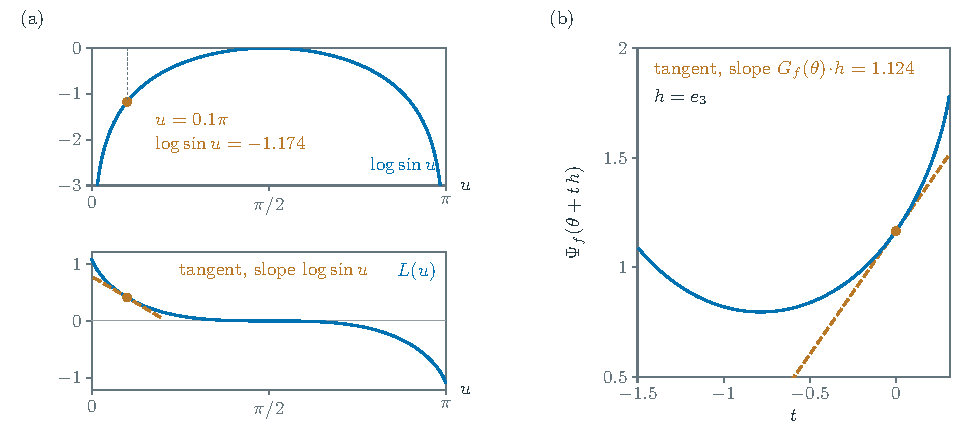
\includegraphics[width=\linewidth]{figures/clh_lean_potential.pdf}
\caption{(a) $\log\sin u$ on $(0,\pi)$ and its primitive $L(u)=\int_{\pi/2}^{u}\log\sin t\,dt$, with the tangent of $L$ at $u=0.1\pi$, of slope $\log\sin u$. (b) $\Psi_f(\theta+t\,h)$, with $L$ normalised as in (a), for $h=e_3$, $\ba=(3,5,1,2,4)$ and $\theta/\pi=(0,0.1,0.7,0.3,0.8)$, over the $t$ for which every gap stays in $(0,\pi)$. The tangent at $t=0$ has slope $G_f(\theta)\cdot h$; the curve lies above it. Numerical values, in floating point.}
\label{fig:clh-lean-potential}
\end{figure}

\begin{proof}
From a point $X=\Meas_f(\theta)\in\Critf$, form the left twist $\widetilde\tau(X)$ (regular on the open
positroid cell, \cite{MullerSpeyer}), read its Grassmann-necklace Pl\"ucker coordinates
$\Delta_{I_r}(\widetilde\tau(X))$ (nonzero on the open cell), and take the vector of logarithms of their
absolute values; the projective scale is removed by passing to differences, i.e.\ to $\im(B)$. This is
$R_f(X)$ as displayed in the statement. Take $\theta$ first in the gauge slice, and let $t$ be the complex parameter of
\eqref{eq:t-of-theta}, so that $\widetilde\tau(X)=\widetilde\tau(\Meas_G(\mathrm{wt}_t))$ by
\eqref{eq:meas-identification} and \eqref{eq:gal512} applies verbatim (the last paragraph of this proof
says why, collisions included). Taking $\log\lvert\cdot\rvert$ of \eqref{eq:gal512} turns the monomial
into a linear form,
\[
   \log\lvert\Delta_{I_r}(\widetilde\tau(X))\rvert
   =\bigl(M_N\,\log\lvert[\![t_q,t_p]\!]_+\rvert\bigr)_r
\]
up to the projective constant, and by Lemma~\ref{lem:hinge}
$\log\lvert[\![t_q,t_p]\!]_+\rvert=\ell_e+\log2$ on every crossing pair (the non-crossing columns of
$M_N$ being zero by Proposition~\ref{prop:rowdiff}, the value assigned there is irrelevant, cf.\
\S\ref{sec:mn}). The cyclic row-difference and $P_f$-relabeling then give, via
Proposition~\ref{prop:rowdiff},
$R_f\circ\Meas_f = P_f D M_N\,(\ell+\log2\cdot\mathbf 1)=B\ell = G_f$; the per-edge constant contributes
$(\log2)\,P_fDM_N\mathbf1=(\log2)\,B\mathbf1=0$, because in-degree equals out-degree at every vertex of
$G_f^{\,x}$ by Proposition~\ref{prop:wp-direct-balance} --- the third and last forward reference from
\S\S\ref{sec:setup}--\ref{sec:gradient} into
\S\ref{sec:wp-combinatorial-bridge}, which is proved there directly from the refined endpoint order and
is independent of everything in this section.
Finally $\partial_\theta\ell_e=\cot\delta_e\,\partial_\theta\delta_e$ and
$\partial_\theta\delta_e=e_q-e_p$ (equation~\eqref{eq:delta-increment}, unaffected by the affine lift)
give $G_f=B\ell=\nabla\Psi_f$ with $\Psi_f$ as in \eqref{eq:potential},
and $\Hess\Psi_f=B\operatorname{diag}(\cot\delta_e)B^{\mathsf T}$.
Figure~\ref{fig:clh-lean-incidence} shows the identity $G_f=B\ell$ on the worked example, label by label.
\begin{figure}[htbp]
\centering
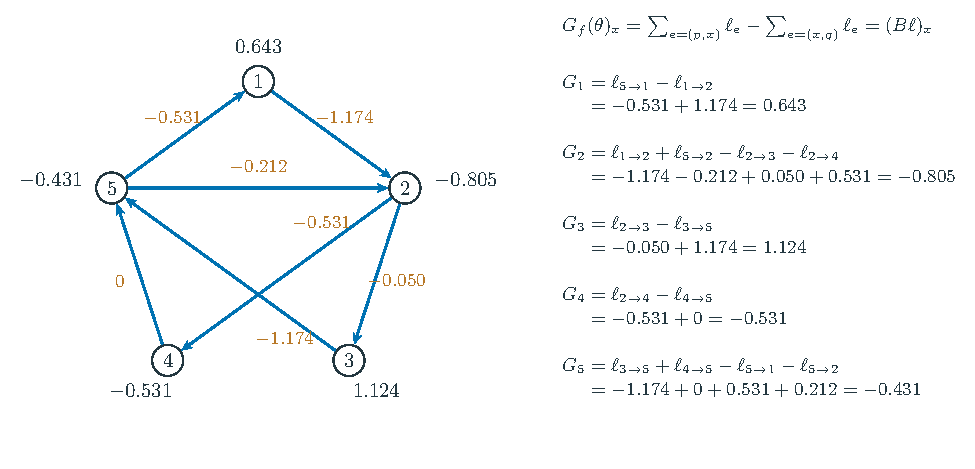
\includegraphics[width=\linewidth]{figures/clh_lean_incidence.pdf}
\caption{The crossing graph of $\ba=(3,5,1,2,4)$ at $\theta/\pi=(0,0.1,0.7,0.3,0.8)$: the weight $\ell_e=\log\sin\delta_e$ on each edge (ochre) and, at each label $x$, the weights into $x$ minus the weights out of $x$ (black), which is $G_f(\theta)_x=(B\ell)_x$. Numerical values, in floating point.}
\label{fig:clh-lean-incidence}
\end{figure}

Where the identity holds. Galashin states Proposition~5.12 for every $t\in\Theta_f^\circ$ at which
$\Meas_G$ is well defined. For $\theta$ in the gauge slice, $t=e^{i\theta}$ lies in $\Theta_f^\circ$:
the slice fixes the component representatives at angle $0$, so $t_{p_1}=\dots=t_{p_{c_f}}=1$, and
admissibility of $\theta$ gives $t_p\ne\pm t_q$ on every crossing pair. And $\Meas_G$ is well defined at
$t$ by \cite[Lem.~5.13]{Galashin}. So the computation above holds at every point of the gauge slice,
including points where two noncrossing labels collide ($t_p=\pm t_q$); no density or continuity
argument is needed. At such a point the vanishing bracket does not occur in the necklace expression,
because colliding labels cannot form a crossing pair and Proposition~\ref{prop:rowdiff} shows that every
noncrossing-pair exponent is zero on every necklace row. And $\Meas_f(\theta)$ stays in the open
positroid cell, where the twist and the nonzero necklace coordinates, hence $R_f$, are defined and
continuous: all interior edge weights are strictly positive at an admissible tuple
\cite[Prop.~4.2]{Galashin}, so $\Meas_f(\theta)\in\Pi_f^{>0}$ \cite[Def.~1.8 and eq.~(2.6)]{Galashin}.
On the ambient chamber the identity follows by a component shift: it moves any $\theta\in\Theadm$ into
the slice without changing $\Meas_f(\theta)$ \cite[Prop.~4.2 and the paragraph following it]{Galashin}
or any $\delta_e$, so neither side of $R_f\circ\Meas_f=G_f$ changes. (A density argument on the locus of
pairwise distinct parameters, which is dense in $\Theadm$, would not serve on the slice itself: when
$c_f\ge2$ the slice fixes all component representatives at the same angle, so that locus does not meet
it.)
\end{proof}

\begin{remark}[recovery from the ordinary necklace minors]\label{rem:untwisted}
The twist is needed to apply \eqref{eq:gal512}, not to evaluate $R_f$. For $A$ in the open positroid cell,
$\Delta_{I_r}(A)=1/\Delta_{I_r}(\widetilde\tau(A))$ for every $r$ \cite[proof of Prop.~5.4]{Galashin}, which
cites \cite[proof of Prop.~6.6]{MullerSpeyer}; a change of representative rescales the necklace minors of
$X$ by one common factor, which $D$ annihilates. Since $(Dz)_r=z_{r+1}-z_r$ and $(P_fz)_x=z_{s_x}$,
\begin{equation}\label{eq:untwisted}
   R_f(X)=-P_fD\Bigl(\log\bigl\lvert\Delta_{I_r}(X)\bigr\rvert\Bigr)_{r=1}^{n},\qquad
   \bigl(R_f(X)\bigr)_x=\log\biggl\lvert\frac{\Delta_{I_{s_x}}(X)}{\Delta_{I_{s_x+1}}(X)}\biggr\rvert,
\end{equation}
with the necklace position $s_x+1$ read cyclically. So the angles are recovered from ratios of the ordinary
Grassmann-necklace minors of $X$, and the twist need not be computed; Corollary~\ref{cor:necklace-embedding}
records the consequence.
\end{remark}

\section{The potential is convex}\label{sec:convex}

\subsection{Existence of winding-one partitions}
Both proofs of the partition below use one counting fact about advances, which we state once. For
distinct $p,q\in[n]$ put $\operatorname{adv}(p,q)=(q-p)\bmod n\in\{1,\ldots,n-1\}$.

\begin{lemma}[Closed walks of advance $n$ are simple]\label{lem:winding-simple}
Let $v_0\to v_1\to\cdots\to v_{m-1}\to v_0$ be a closed walk of labels in $[n]$ (or in
$\mathbb Z_n$, as in \S\ref{sec:wp-combinatorial-bridge}) with $m\ge2$ and consecutive vertices
distinct. Its total advance $\sum_i\operatorname{adv}(v_i,v_{i+1})$ (indices modulo $m$) is a
positive multiple of $n$. If it equals $n$, the vertices $v_0,\dots,v_{m-1}$ are pairwise distinct.
\end{lemma}

\begin{proof}
Each advance is at least $1$, and modulo $n$ the advances telescope:
$\sum_i\operatorname{adv}(v_i,v_{i+1})\equiv\sum_i(v_{i+1}-v_i)=0$. If $v_i=v_j$ with $0\le i<j\le m-1$,
the walk splits at that vertex into the closed walks $v_i\to\cdots\to v_j$ and
$v_j\to\cdots\to v_{m-1}\to v_0\to\cdots\to v_i$, with $j-i\ge1$ and $m-(j-i)\ge1$ edges. Each has a
total advance that is a positive multiple of $n$, so the whole walk has advance at least $2n$.
\end{proof}

\begin{proposition}[W-P]\label{prop:wp}
For every loopless $f$, the directed crossing-edge set $E_f$ of $G_f^{\,x}$ admits a
partition $\mathcal Z$ into edge-disjoint, vertex-simple directed cycles, each of total
exit-advance $n$ (\emph{winding one}) and length $\ge3$.
Every such partition has the same number of cycles:
\begin{equation}\label{eq:wp-cycle-count}
 |\mathcal Z|=\frac1n\sum_{(p,q)\in E_f}\operatorname{adv}(p,q)
 =\#\{(p,q)\in E_f:p>q\},
 \qquad \operatorname{adv}(p,q)=(q-p)\bmod n\in\{1,\ldots,n-1\}.
\end{equation}
The partition itself need not be unique.
\end{proposition}

Proposition~\ref{prop:wp} is proved in \S\ref{sec:wp-combinatorial-bridge}, by a finite window induction
from the refined endpoint order alone; that is the proof Lean checks. A second, geometric proof from a
reduced alternating strand diagram follows in \S\ref{sec:wp-strand}. Nothing later in the paper depends on
which of the two is used.


\paragraph{Choice of partition and scope of the combinatorics.}
For example, the loopless window $f=(3,5,6,7,9)$ has directed crossing edges
\[
 E_f=\{(1,2),(2,3),(2,4),(3,5),(4,5),(5,1),(5,2)\}.
\]
Two distinct winding-one partitions are
\[
 \{(1,2,3,5),(2,4,5)\}
 \quad\text{and}\quad
 \{(1,2,4,5),(2,3,5)\},
\]
where each tuple denotes a cyclic vertex list. Each partition has two cycles,
matching the two wrapped edges $(5,1)$ and $(5,2)$. The Hessian decomposition
below may use any fixed winding-one partition.
Figure~\ref{fig:clh-partitions} draws both choices; Appendix~\ref{app:worked-example} gives the necklace rows and matrices for the same window.

\begin{figure}[htbp]
\centering
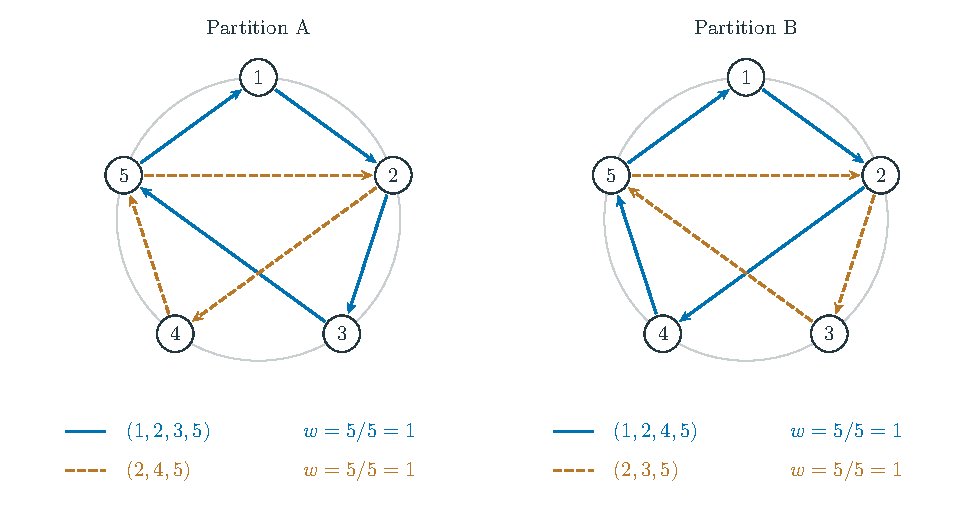
\includegraphics[width=\linewidth]{figures/clh_partitions.pdf}
\caption{Two winding-one partitions for $f=(3,5,6,7,9)$. In each panel the blue solid cycle and the ochre dashed cycle together use every directed crossing edge exactly once. Each cycle has total cyclic advance $5$, hence winding $w=5/5=1$. The partitions differ in how the edges through labels $3$ and $4$ are assigned to cycles.}
\label{fig:clh-partitions}
\end{figure}

Figure~\ref{fig:clh-lean-wp-count} counts the cycles of \eqref{eq:wp-cycle-count} for the two partitions of Figure~\ref{fig:clh-partitions}.

\begin{figure}[htbp]
\centering
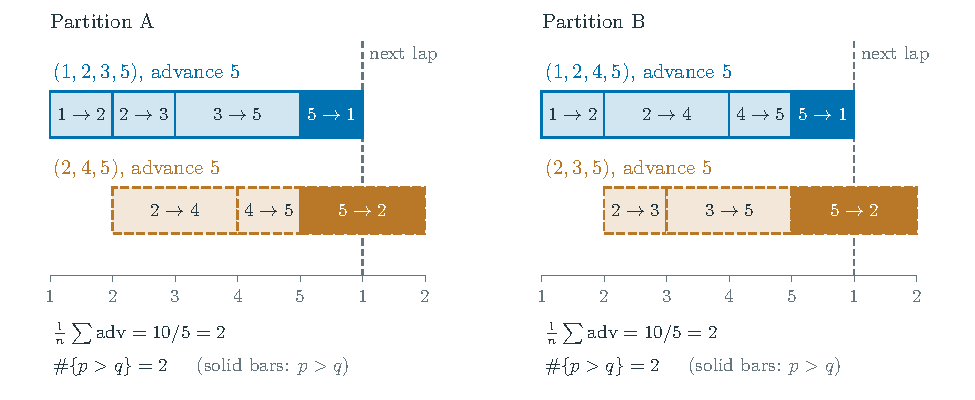
\includegraphics[width=\linewidth]{figures/clh_lean_wp_count.pdf}
\caption{The count \eqref{eq:wp-cycle-count} for the two partitions of Figure~\ref{fig:clh-partitions}, $f=(3,5,6,7,9)$. A cycle is a bar of length its total advance $5$, cut into the advances $\operatorname{adv}(p,q)$ of its edges; solid bars are the edges with $p>q$, and the positions run on past label $5$ into the next lap. Both partitions have total advance $10=5\cdot2$ and two edges with $p>q$, $(5,1)$ and $(5,2)$. The advances are counted directly.}
\label{fig:clh-lean-wp-count}
\end{figure}

The refined-endpoint crossing rule depends only on the induced permutation
$\ba$, not on the decoration of its fixed points. Every permutation has a
loopless bounded affine lift, obtained by choosing $p<f(p)\le p+n$; a fixed
point then has $f(p)=p+n$. Thus the purely combinatorial partition statement
also holds for every decorated permutation, by applying the proposition to
that lift. Fixed-point decorations do not alter the directed edge set or its
advances. This observation does not extend the critical measurement theorem
to looped cells; its domain remains the one in Theorem~\ref{thm:main}.


\subsection{A combinatorial proof of partition existence}
\label{sec:wp-combinatorial-bridge}


This subsection proves Proposition~\ref{prop:wp} from the refined endpoint order
alone, by a finite induction. It uses no strand diagram and no plabic-graph citation.

Let
\[
   \mathbb Z_n=\{0,\ldots,n-1\}
\]
with its cyclic order, and let \(\sigma\) be a permutation of
\(\mathbb Z_n\). Put \(s=\sigma^{-1}\). At each boundary position \(i\)
retain two distinct refined points \(i^-,i^+\), in that clockwise order.
For \(p\in\mathbb Z_n\), the chord \(C_p\) is directed from \(s(p)^+\) to
\(p^-\). For distinct \(p,q\), write \(p\to q\) when
\begin{equation}
   s(p)^+,\ s(q)^+,\ p^-,\ q^-
   \label{eq:wp-directed-crossing}
\end{equation}
occur in clockwise cyclic order. Denote the resulting directed edge set by
\(E(\sigma)\), and put
\[
   \operatorname{adv}(p,q)=(q-p)\bmod n\in\{1,\ldots,n-1\}.
\]
The winding of a directed closed walk is its total advance divided by \(n\).

To bridge conventions, identify the \(0\)-based permutation \(\sigma\) of
\(\mathbb Z_n\) used here with the paper's induced permutation \(\ba\) (under
\(x\mapsto x+1\)), so that \(s=\sigma^{-1}\) becomes \(s_x=\ba^{-1}(x)\). Since
\(f\) is loopless, the fixed points of \(\sigma\) are its coloops.  The
directed edge set \(E(\sigma)\) is then exactly the directed crossing-edge set of
\(G_f^{\,x}\): both are read from the same \(\varepsilon\)-resolved endpoint order,
in which each exit \(i^-\) occurs immediately before the entry \(i^+\) at boundary
position \(i\), and the relation \(p\to q\) of \eqref{eq:wp-directed-crossing}
is precisely Galashin's clockwise crossing order
\(b^+_{s_p},b^+_{s_q},b^-_p,b^-_q\).  Establishing that \(E(\sigma)\) is an
edge-disjoint union of vertex-simple winding-one cycles, each of length at least
\(3\), therefore proves Proposition~\ref{prop:wp}.

We first record a direct consequence of the refined endpoint convention.

\begin{proposition}[Direct degree balance]
\label{prop:wp-direct-balance}
For every \(p\in\mathbb Z_n\),
\[
   \operatorname{outdeg}_{E(\sigma)}(p)
   =
   \operatorname{indeg}_{E(\sigma)}(p).
\]
\end{proposition}

\begin{proof}
Fix \(p\), and let
\[
   U_p=(s(p)^+,p^-)
\]
be the open clockwise refined interval. This interval contains whole pairs
\(r^-,r^+\): after leaving \(s(p)^+\), every intermediate boundary position
is encountered first at \(r^-\) and then at \(r^+\), while the two endpoints
of \(U_p\) themselves are excluded. Consequently \(U_p\) contains equally
many entry points and exit points.

For \(q\ne p\), the cyclic-order definition gives
\[
\begin{aligned}
   p\to q
   &\quad\Longleftrightarrow\quad
   s(q)^+\in U_p\ \text{ and }\ q^-\notin U_p,\\
   q\to p
   &\quad\Longleftrightarrow\quad
   q^-\in U_p\ \text{ and }\ s(q)^+\notin U_p.
\end{aligned}
\]
If both endpoints of \(C_q\) lie in \(U_p\), or both lie outside it, the two
chords do not cross. Hence
\[
\begin{aligned}
  \operatorname{outdeg}(p)-\operatorname{indeg}(p)
   &=
   \sum_{q\in\mathbb Z_n}
   \left(
      \mathbf 1_{\{s(q)^+\in U_p\}}
      -
      \mathbf 1_{\{q^-\in U_p\}}
   \right)\\
   &=
   \#\{\text{entry points in }U_p\}
   -
   \#\{\text{exit points in }U_p\}
   =0.
\end{aligned}
\]
\end{proof}

We now enlarge the finite state space used in the induction. A
\emph{decorated bounded window} is an integer tuple
\[
   w=(w_0,\ldots,w_{n-1})
\]
such that the residues
\[
   \bar w_i:=w_i\bmod n\in\mathbb Z_n
\]
form a permutation and
\begin{equation}
   i\le w_i\le i+n
   \qquad(0\le i<n).
   \label{eq:wp-window-bounds}
\end{equation}
A position \(i\) is \emph{fixed} if \(\bar w_i=i\), and \emph{active}
otherwise. At a fixed position one has either \(w_i=i\) or \(w_i=i+n\).
The residue permutation determines an inverse \(s_w\), and we define \(E(w)\)
by the same rule as in \eqref{eq:wp-directed-crossing}, with \(s_w\) in place
of \(s\). The two decorations of a fixed position give the same refined
chord: its endpoints \(i^-,i^+\) are adjacent, so it crosses no other chord.

The original permutation gives the bounded window
\begin{equation}
   w_i^\sigma=
   \begin{cases}
      \sigma(i),&\sigma(i)>i,\\
      \sigma(i)+n,&\sigma(i)\le i,
   \end{cases}
   \label{eq:wp-derangement-lift}
\end{equation}
which is the window of \(f\) in \(0\)-based labels; a coloop \(i\) gets the
decoration \(w_i^\sigma=i+n\). Then \(i<w_i^\sigma\le i+n\), its residue permutation is \(\sigma\), and
\begin{equation}
   E(w^\sigma)=E(\sigma).
   \label{eq:wp-lift-same-edges}
\end{equation}

\begin{lemma}[Active-set restriction]
\label{lem:wp-active-set}
The residue permutation \(i\mapsto\bar w_i\) restricts to a permutation of the
active positions.
\end{lemma}

\begin{proof}
If \(i\) is fixed, then the residue \(i\) already occurs at position \(i\).
Since all residues are distinct, no other position can map to \(i\). Thus the
fixed positions map bijectively to themselves, and their complement does as
well.
\end{proof}

\begin{lemma}[Adjacent active ascent]
\label{lem:wp-adjacent-active-ascent}
If \(w\) has an active position, there are adjacent positions \(a<b\) in the
increasing list of active positions such that
\[
   A:=w_a<B:=w_b.
\]
Every \(r\) with \(a<r<b\) is fixed, and
\begin{equation}
   b\le A<B\le a+n.
   \label{eq:wp-bridge-bounds}
\end{equation}
If \(g\) is obtained by swapping \(A\) and \(B\) at positions \(a,b\), then
\(g\) is again a decorated bounded window.
\end{lemma}

\begin{proof}
Write the active positions as
\[
   i_1<\cdots<i_m.
\]
If \(m>0\), then \(m\ge2\), since a permutation cannot move exactly one
element. By Lemma~\ref{lem:wp-active-set}, the residue at \(i_1\) is another
active position and therefore is strictly larger than \(i_1\); similarly, the
residue at \(i_m\) is strictly smaller than \(i_m\). Boundedness forces
\[
   w_{i_1}=\bar w_{i_1}\le i_m
   <i_1+n\le \bar w_{i_m}+n=w_{i_m}.
\]
Thus the sequence \(w_{i_1},\ldots,w_{i_m}\) cannot be strictly decreasing,
so some adjacent pair in it is an ascent. Choose such a pair and call its
positions \(a<b\). Their adjacency in the active list says precisely that
every \(a<r<b\) is fixed.

Put
\[
   \alpha=A\bmod n,\qquad \beta=B\bmod n.
\]
The label \(\alpha\) is active, so \(\alpha\ne a\). If \(\alpha<a\), boundedness gives
\(A=\alpha+n\ge b\); if \(\alpha>a\), adjacency of \(a,b\) in the active list
gives \(\alpha\ge b\), and boundedness then forces \(A=\alpha\). Thus
\(b\le A\). Similarly, if \(\beta<b\), then \(\beta\le a\) and
\(B=\beta+n\le a+n\); if \(\beta>b\), then \(B=\beta\le n-1<a+n\).
This proves \eqref{eq:wp-bridge-bounds}.

After the swap, the value at \(a\) is \(B\), and
\[
   a<B\le a+n.
\]
The value at \(b\) is \(A\), and
\[
   b\le A<B\le a+n<b+n.
\]
The residues are unchanged as a set, so the swapped tuple is again a decorated
bounded window.
\end{proof}

Define
\begin{equation}
   \operatorname{inv}(w)
   =
   \#\{(i,j):0\le i<j<n,\ w_i>w_j\},
   \qquad
   \mu(w)=\binom n2-\operatorname{inv}(w).
   \label{eq:wp-measure}
\end{equation}

\begin{lemma}[Strict measure decrease]
\label{lem:wp-measure-decrease}
For the swap \(w\mapsto g\) in
Lemma~\ref{lem:wp-adjacent-active-ascent},
\begin{equation}
   \operatorname{inv}(g)=\operatorname{inv}(w)+1,
   \qquad
   \mu(g)=\mu(w)-1.
   \label{eq:wp-measure-drop}
\end{equation}
\end{lemma}

\begin{proof}
For \(a<r<b\), fixedness gives either \(w_r=r\) or \(w_r=r+n\). In the first
case,
\[
   w_r=r<b\le A;
\]
in the second,
\[
   w_r=r+n>a+n\ge B.
\]
Thus no intermediate value belongs to \([A,B]\).

The pair \((a,b)\) changes from the noninversion \(A<B\) to an inversion.
For an intermediate position \(r\), the total inversion contribution of
\((a,r)\) and \((r,b)\) is unchanged: its value lies either below both \(A,B\)
or above both. A position outside \([a,b]\) sees the same two-element multiset
\(\{A,B\}\) on the same side. Hence exactly one inversion is added, proving
\eqref{eq:wp-measure-drop}.
\end{proof}

We next give the exact change in the directed crossing graph. For an integer
lift \(r\), define
\begin{equation}
   \kappa(r^-)=2r,\qquad
   \kappa(r^+)=2r+1.
   \label{eq:wp-kappa}
\end{equation}
Thus
\[
   \kappa((r+n)^\varepsilon)
   =
   \kappa(r^\varepsilon)+2n,
   \qquad \varepsilon\in\{-,+\}.
\]
Write \(x\prec y\) when the chosen integer lifts satisfy
\(\kappa(x)<\kappa(y)\). A chain of four such inequalities contained in one
interval of \(\kappa\)-length \(2n\) records their clockwise cyclic order.

When displaying endpoint orders, the integer before the subscript records the
chosen lift position, while the subscript records the chord label. Thus
\(r_p^+\) denotes the entry point of \(C_p\) represented at integer position
\(r\), so \(r\equiv s_w(p)\pmod n\), and \(r_p^-\) denotes the exit point of
\(C_p\) represented at integer position \(r\), so \(r\equiv p\pmod n\).
The subscript does not enter the order coordinate:
\[
   \kappa(r_p^\varepsilon)=\kappa(r^\varepsilon),
   \qquad \varepsilon\in\{-,+\}.
\]
The label attached to a fixed refined position is always read in the state
\(w\) or \(g\) currently under discussion.

Figure~\ref{fig:clh-window} draws the lemma below. Cut the circle just before
\(a^+\) and lift one turn: the swap moves only the entries of \(\alpha\) and
\(\beta\) between \(a^+\) and \(b^+\), the open swept arc between them holds
\(b^-\) and the isolated chords of fixed positions, and the three regimes are
the three places of the entry \(S^+\) of the chord \(C_b\) relative to the
exits \(A^-\) and \(B^-\).

\begin{figure}[t]
\centering
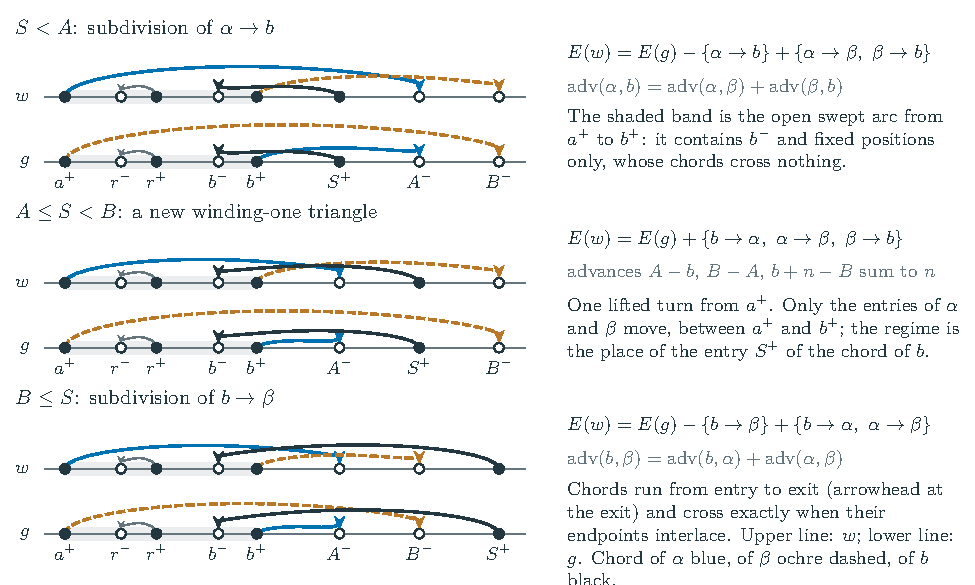
\includegraphics[width=\linewidth]{figures/clh_window_transition.pdf}
\caption{The three regimes of Lemma~\ref{lem:wp-local-transition}, on one lifted turn starting at $a^+$. Chords run from entry to exit; two chords cross exactly when their endpoints interlace. In each regime the upper line carries the chords of $w$ and the lower line those of $g$; only the entries of $\alpha$ and $\beta$ differ. The shaded band is the open swept arc from $a^+$ to $b^+$. Schematic; the positions are illustrative.}
\label{fig:clh-window}
\end{figure}

\begin{lemma}[Exact local transition]
\label{lem:wp-local-transition}
Use the notation of Lemma~\ref{lem:wp-adjacent-active-ascent}. If \(A=b\),
then
\begin{equation}
   E(w)=E(g).
   \label{eq:wp-transition-identity}
\end{equation}
Assume \(A>b\). Let \(c=s_w(b)\), and define
\begin{equation}
   S=
   \begin{cases}
      c+n,&c<a,\\
      c,&c>b.
   \end{cases}
   \label{eq:wp-S-lift}
\end{equation}
Then \(b<S<a+n\), and exactly one of the following holds:
\begin{equation}
   S<A:\quad
   E(w)
   =
   \bigl(E(g)\setminus\{\alpha\to b\}\bigr)
   \cup\{\alpha\to\beta,\beta\to b\},
   \label{eq:wp-transition-left}
\end{equation}
\begin{equation}
   A\le S<B:\quad
   E(w)
   =
   E(g)\cup\{b\to\alpha,\alpha\to\beta,\beta\to b\},
   \label{eq:wp-transition-triangle}
\end{equation}
\begin{equation}
   B\le S:\quad
   E(w)
   =
   \bigl(E(g)\setminus\{b\to\beta\}\bigr)
   \cup\{b\to\alpha,\alpha\to\beta\}.
   \label{eq:wp-transition-right}
\end{equation}
Every displayed added edge is absent from \(E(g)\), and every displayed
removed edge is absent from \(E(w)\).
\end{lemma}

\begin{proof}
Only the entries of the labels \(\alpha,\beta\) move:
\begin{equation}
\begin{array}{c|cc}
   &s(\alpha)&s(\beta)\\ \hline
 w&a&b\\
 g&b&a.
\end{array}
\label{eq:wp-entry-swap}
\end{equation}
We first justify that no unlisted label can affect the transition.

The open refined arc from \(a^+\) to \(b^+\) contains \(b^-\), but it does not
contain \(a^-\): at each position the order is \(r^-,r^+\). It also contains
both endpoints \(r^-,r^+\) of every strictly intermediate position
\(a<r<b\). Such a position is fixed, and its adjacent-endpoint chord is
isolated in both \(E(w)\) and \(E(g)\).

Now let \(q\) be active and
\[
   q\notin\{b,\alpha,\beta\}.
\]
By Lemma~\ref{lem:wp-active-set}, the exit label \(q\) is itself an active
position. Since \(a,b\) are adjacent active positions, \(q^-\) is not in the
open arc from \(a^+\) to \(b^+\); the possibility \(q=a\) causes no exception,
because \(a^-\) precedes \(a^+\). Likewise, \(s_w(q)\) is an active position.
It is neither \(a\) nor \(b\), since the entries there belong to
\(\alpha,\beta\), and it cannot lie strictly between them. Thus
\(s_w(q)^+\) is outside the swept arc. The same is true in \(g\), since the
inverse position of \(q\) does not change.

For a pair involving \(\alpha\) and such a \(q\), the three stationary
endpoints are \(\alpha^-,s(q)^+,q^-\). Except when \(\alpha=b\), which is the
separate case \(A=b\), none lies in the swept arc. The analogous assertion
holds for \(\beta\) and \(q\); if \(\beta=a\), its exit is \(a^-\), again
outside the arc. In a finite cyclic order, deleting three stationary points
partitions the remaining points into three cyclic intervals. The points
\(a^+\) and \(b^+\) lie in the same such interval whenever the open arc
between them contains none of the three stationary points. Replacing one by
the other therefore leaves the labeled cyclic order of the four endpoints
unchanged. Hence only pairs contained in
\[
   \{b,\alpha,\beta\}
\]
can change. In particular, the label \(a\) is never an additional special
label: its exit \(a^-\) is outside the swept arc, and if \(a=\beta\) it is
already included in the displayed set.

Suppose first that \(A=b\), so \(\alpha=b\). Since \(A<B\le a+n\), the four
endpoints of the only special pair \(\{b,\beta\}\) occur in \(w\) as
\begin{equation}
   a_b^+
   \prec
   b_b^-
   \prec
   b_\beta^+
   \prec
   B_\beta^-.
   \label{eq:wp-Aeqb-w}
\end{equation}
The two endpoints of \(b\) are consecutive in this four-point order, as are
the two endpoints of \(\beta\), so the pair is noncrossing. In \(g\), their
order is
\begin{equation}
   a_\beta^+
   \prec
   b_b^-
   \prec
   b_b^+
   \prec
   B_\beta^-.
   \label{eq:wp-Aeqb-g}
\end{equation}
which is again noncrossing. This proves
\eqref{eq:wp-transition-identity}.

Assume henceforth that \(A>b\). Then \(\alpha,\beta,b\) are distinct. The
entry position \(c=s_w(b)\) is active. It is not \(a\), because
\(\alpha\ne b\), and it is not \(b\), because \(b\) is active. It cannot lie
strictly between \(a,b\), so \eqref{eq:wp-S-lift} is well defined and gives
\begin{equation}
   b<S<a+n.
   \label{eq:wp-S-bounds}
\end{equation}
The relevant exit lifts satisfy
\begin{equation}
   b<A<B<b+n.
   \label{eq:wp-special-exit-order}
\end{equation}

For the pair \(\{\alpha,\beta\}\), independently of the position of \(S\),
the order in \(w\) is
\begin{equation}
   a_\alpha^+
   \prec
   b_\beta^+
   \prec
   A_\alpha^-
   \prec
   B_\beta^-.
   \label{eq:wp-alphabeta-w}
\end{equation}
This is exactly the defining order for \(\alpha\to\beta\). In \(g\), the
order is
\begin{equation}
   a_\beta^+
   \prec
   b_\alpha^+
   \prec
   A_\alpha^-
   \prec
   B_\beta^-.
   \label{eq:wp-alphabeta-g}
\end{equation}
The two \(\alpha\)-endpoints are consecutive in this four-point order, so the
pair is noncrossing. Thus \(\alpha\to\beta\) belongs to
\(E(w)\setminus E(g)\) in all three regimes.

We now inspect the two remaining pairs in each regime.

\smallskip
\noindent\emph{Case \(S<A\).}
For \(\{\alpha,b\}\), the endpoint order in \(w\) is
\begin{equation}
   b_b^-
   \prec
   S_b^+
   \prec
   A_\alpha^-
   \prec
   (a+n)_\alpha^+.
   \label{eq:wp-left-alphab-w}
\end{equation}
The two \(b\)-endpoints and the two \(\alpha\)-endpoints are each consecutive,
so the pair is noncrossing. In \(g\), the order is
\begin{equation}
   b_\alpha^+
   \prec
   S_b^+
   \prec
   A_\alpha^-
   \prec
   (b+n)_b^-.
   \label{eq:wp-left-alphab-g}
\end{equation}
which is the defining order for \(\alpha\to b\).

For \(\{\beta,b\}\), the order in \(w\) is
\begin{equation}
   b_\beta^+
   \prec
   S_b^+
   \prec
   B_\beta^-
   \prec
   (b+n)_b^-.
   \label{eq:wp-left-betab-w}
\end{equation}
so \(\beta\to b\). In \(g\), the order is
\begin{equation}
   S_b^+
   \prec
   B_\beta^-
   \prec
   (a+n)_\beta^+
   \prec
   (b+n)_b^-.
   \label{eq:wp-left-betab-g}
\end{equation}
Here the two \(\beta\)-endpoints are consecutive, so the pair is noncrossing.
Together with \eqref{eq:wp-alphabeta-w}--\eqref{eq:wp-alphabeta-g}, these
orders prove \eqref{eq:wp-transition-left}.

\smallskip
\noindent\emph{Case \(A\le S<B\).}
For \(\{\alpha,b\}\), the endpoint order in \(w\) is
\begin{equation}
   S_b^+
   \prec
   (a+n)_\alpha^+
   \prec
   (b+n)_b^-
   \prec
   (A+n)_\alpha^-.
   \label{eq:wp-middle-alphab-w}
\end{equation}
which is the defining order for \(b\to\alpha\). In \(g\), the order is
\begin{equation}
   b_\alpha^+
   \prec
   A_\alpha^-
   \prec
   S_b^+
   \prec
   (b+n)_b^-.
   \label{eq:wp-middle-alphab-g}
\end{equation}
The two \(\alpha\)-endpoints are consecutive, so the pair is noncrossing.
When \(S=A\), the strict middle inequality in
\eqref{eq:wp-middle-alphab-g} is still valid because
\(A^-\prec A^+\).

For \(\{\beta,b\}\), the endpoint order in \(w\) is
\begin{equation}
   b_\beta^+
   \prec
   S_b^+
   \prec
   B_\beta^-
   \prec
   (b+n)_b^-.
   \label{eq:wp-middle-betab-w}
\end{equation}
so \(\beta\to b\). In \(g\), the order is
\begin{equation}
   S_b^+
   \prec
   B_\beta^-
   \prec
   (a+n)_\beta^+
   \prec
   (b+n)_b^-.
   \label{eq:wp-middle-betab-g}
\end{equation}
which is noncrossing because the two \(\beta\)-endpoints are consecutive.
Together with \eqref{eq:wp-alphabeta-w}--\eqref{eq:wp-alphabeta-g}, these
orders prove \eqref{eq:wp-transition-triangle}.

\smallskip
\noindent\emph{Case \(B\le S\).}
For \(\{\alpha,b\}\), the endpoint order in \(w\) is again
\begin{equation}
   S_b^+
   \prec
   (a+n)_\alpha^+
   \prec
   (b+n)_b^-
   \prec
   (A+n)_\alpha^-.
   \label{eq:wp-right-alphab-w}
\end{equation}
so \(b\to\alpha\). In \(g\), the order is
\begin{equation}
   b_\alpha^+
   \prec
   A_\alpha^-
   \prec
   S_b^+
   \prec
   (b+n)_b^-.
   \label{eq:wp-right-alphab-g}
\end{equation}
so the pair is noncrossing.

For \(\{\beta,b\}\), the endpoint order in \(w\) is
\begin{equation}
   b_\beta^+
   \prec
   B_\beta^-
   \prec
   S_b^+
   \prec
   (b+n)_b^-.
   \label{eq:wp-right-betab-w}
\end{equation}
The two \(\beta\)-endpoints are consecutive, so the pair is noncrossing. In
\(g\), the order is
\begin{equation}
   S_b^+
   \prec
   (a+n)_\beta^+
   \prec
   (b+n)_b^-
   \prec
   (B+n)_\beta^-.
   \label{eq:wp-right-betab-g}
\end{equation}
which is the defining order for \(b\to\beta\). When \(S=B\), the exit
\(B^-\) precedes the entry \(B^+\), so the first \(\beta\)-exit encountered
after \(S_b^+=B_b^+\) is \((B+n)_\beta^-\); this is why equality belongs to
the third regime. Together with
\eqref{eq:wp-alphabeta-w}--\eqref{eq:wp-alphabeta-g}, these orders prove
\eqref{eq:wp-transition-right}.
\end{proof}

\begin{lemma}[Winding arithmetic]
\label{lem:wp-winding-arithmetic}
In the triangle case \eqref{eq:wp-transition-triangle},
\[
   b\to\alpha\to\beta\to b
\]
has winding one. In each subdivision case, the two-edge replacement has the
same total advance as the removed edge.
\end{lemma}

\begin{proof}
By \eqref{eq:wp-special-exit-order},
\[
\begin{aligned}
   \operatorname{adv}(b,\alpha)&=A-b,\\
   \operatorname{adv}(\alpha,\beta)&=B-A,\\
   \operatorname{adv}(\beta,b)&=b+n-B.
\end{aligned}
\]
Their sum is \(n\), proving the triangle assertion. In the left subdivision,
\[
\begin{aligned}
   \operatorname{adv}(\alpha,b)
   &=b+n-A\\
   &=(B-A)+(b+n-B)\\
   &=\operatorname{adv}(\alpha,\beta)
     +\operatorname{adv}(\beta,b).
\end{aligned}
\]
In the right subdivision,
\[
\begin{aligned}
   \operatorname{adv}(b,\beta)
   &=B-b\\
   &=(A-b)+(B-A)\\
   &=\operatorname{adv}(b,\alpha)
     +\operatorname{adv}(\alpha,\beta).
\end{aligned}
\]
\end{proof}

\begin{proof}[Proof of Proposition~\ref{prop:wp}]
The induction establishes the stronger statement for every decorated bounded
window \(w\): \(E(w)\) is an edge-disjoint union of winding-one directed
cycles. It is a strong induction on the nonnegative integer \(\mu(w)\) from
\eqref{eq:wp-measure}.

If \(w\) has no active position, its residue permutation is the identity.
Thus each \(w_i\) is either \(i\) or \(i+n\), every chord has adjacent
endpoints \(i^-,i^+\), and
\[
   E(w)=\varnothing.
\]
Conversely, a state with an active position cannot be terminal:
Lemma~\ref{lem:wp-adjacent-active-ascent} supplies an adjacent active ascent.
Thus the all-fixed windows are exactly the terminal states of the reduction.

Suppose \(w\) is not terminal. Choose \(a,b\) as in
Lemma~\ref{lem:wp-adjacent-active-ascent}, and let \(g\) be the swapped
window. Lemma~\ref{lem:wp-measure-decrease} gives \(\mu(g)<\mu(w)\), so the
induction hypothesis supplies an edge-disjoint partition of \(E(g)\) into
winding-one directed cycles.

In the identity case \eqref{eq:wp-transition-identity}, retain this partition.
In the triangle case \eqref{eq:wp-transition-triangle}, add
\[
   b\to\alpha\to\beta\to b
\]
as a new part; it winds once by Lemma~\ref{lem:wp-winding-arithmetic}.

Consider the left subdivision \eqref{eq:wp-transition-left}. The edge
\(\alpha\to b\) has a unique owner cycle in the partition of \(E(g)\).
Replace that occurrence by
\[
   \alpha\to\beta\to b.
\]
The new edges belong to \(E(w)\setminus E(g)\), so they occur nowhere else in
the old partition, and Lemma~\ref{lem:wp-winding-arithmetic} preserves the
total advance. The labels \(\alpha,\beta,b\) are distinct. The substituted
closed walk has total advance \(n\), so it is vertex-simple by
Lemma~\ref{lem:winding-simple}; in particular the inserted vertex \(\beta\)
does not already occur elsewhere in the owner cycle.

The right subdivision \eqref{eq:wp-transition-right} is identical: replace
the uniquely owned edge \(b\to\beta\) by
\[
   b\to\alpha\to\beta.
\]
The inserted label \(\alpha\) is distinct from \(b,\beta\), the two new edges
are absent from \(E(g)\), the advance is preserved, and
Lemma~\ref{lem:winding-simple} again shows that the new owner cycle is
vertex-simple.

In every case the resulting cycles are edge-disjoint and exhaust \(E(w)\).
This completes the induction. Applying it to \(w^\sigma\) and using
\eqref{eq:wp-lift-same-edges} proves the required decomposition of
\(E(\sigma)\).

Next, a vertex-simple directed cycle of winding one is a rotation of the
increasing order of its support. Indeed, for representatives
\(v_i\in\{0,\ldots,n-1\}\),
\[
   \sum_i\operatorname{adv}(v_i,v_{i+1})
   =
   n\cdot
   \#\{i:v_{i+1}<v_i\},
\]
because the ordinary differences telescope. Winding one therefore means
that the cycle has exactly one descent; rotating to begin immediately after
that descent makes its labels strictly increasing. No resulting cycle has
length \(1\), since the crossing graph is irreflexive, or length \(2\), since
it is antisymmetric: for distinct \(p,q\) the four refined points
\(s(p)^+,s(q)^+,p^-,q^-\) are all distinct, and the clockwise pattern
witnessing \(q\to p\) is not a cyclic rotation of the one witnessing
\(p\to q\), so the two cannot hold at once. Thus every support has
cardinality at least \(3\).
Finally, summing $\operatorname{adv}(p,q)=q-p+n\mathbf1_{p>q}$ around each
cycle gives exactly one wrapped edge per cycle, proving the count in
\eqref{eq:wp-cycle-count} as well.
\end{proof}

\begin{remark}
The degree-balance proposition (Proposition~\ref{prop:wp-direct-balance})
proves in- and out-degree balance of the directed crossing graph directly
from the refined endpoint order, without the cycle decomposition; it is in
this form that the gradient identity uses it (Proposition~\ref{prop:grad}).
\end{remark}

\begin{remark}[Machine verification]\label{rem:machine}
Three components of the proof have Lean formalizations: the cotangent cycle
inequality (Lemma~\ref{lem:cot}), which is analytic, and two combinatorial
statements over every loopless $f$, coloops included: the row-difference
identity (Proposition~\ref{prop:rowdiff}) and the
winding-one partition (Proposition~\ref{prop:wp}). The row-difference identity
is formalized in full: crossing columns, the isolation, necklace-membership and
zero-row facts for coloops, and, through
\texttt{Conj43.\allowbreak pairExponent\_\allowbreak nonCross},
\texttt{Conj43.\allowbreak full\_\allowbreak pair\_\allowbreak columns\_\allowbreak zero} and
\texttt{Conj43.\allowbreak rowdiff\_\allowbreak full\_\allowbreak pairs},
noncrossing-column vanishing and the full unordered-pair identity. The winding
partition is formalized via the window induction of this subsection, together
with both forms of the cycle count \eqref{eq:wp-cycle-count} and the
extension to decorated permutations; the strand-diagram proof is not formalized. The auxiliary cover
theorem of that proof (\emph{Existence of a winding-one partition} in Appendix~\ref{app:lean-interface})
is a further named Lean result, not a further mathematical component.

The analytic steps are formalized as well: the lifted cycle sum
\eqref{eq:cycle-sum}, the hinge identity (Lemma~\ref{lem:hinge}), the assembled
Hessian with its positivity and kernel (Proposition~\ref{prop:psd}), the
potential's gradient $B\ell$ and Hessian $B\operatorname{diag}(\cot\delta_e)B^{\mathsf T}$,
strict convexity on the gauge slice, an injective gradient that is an open
embedding into $\im B$, the variational inverse \eqref{eq:variational-inverse},
and the computation that turns the logarithm of \eqref{eq:gal512} on necklace
rows into $G_f$ (Proposition~\ref{prop:grad}). These compose into a
\emph{conditional} form of Theorem~\ref{thm:main}: if a map on the gauge slice
is continuous and onto a set $\mathrm{Crit}$, and a continuous map $N$ on
$\mathrm{Crit}$ satisfies, along it, the logarithmic necklace-row form of
\eqref{eq:gal512}, then the first map is a homeomorphism, with inverse
$G_f^{-1}\circ P_fD\circ N$. Appendix~\ref{app:lean-interface} states these
hypotheses in mathematical notation and names the results of \cite{Galashin}
and \cite{MullerSpeyer} that they stand for. The interface with the definitions
of \cite{Galashin} is formalized as well: against Lean transcriptions of those
definitions, the encoding used here is a bijection onto his loopless bounded
affine permutations, its necklace rows are given by his affine formula, its
crossings and misalignment classes are his, its exponent table is that of
\eqref{eq:gal512}, and Lemma~\ref{lem:halfopen} holds on his refined boundary.
Lean constructs neither the measurement map nor the twist, so it certifies
components, their interface and a conditional composition, not
Theorem~\ref{thm:main} itself; whether the transcribed definitions and the
hypotheses say what \cite{Galashin} and \cite{MullerSpeyer} say is for the
reader to check. Two later results are formalized, the first in full. Of the sharp modulus, Lean has
Theorem~\ref{thm:sharp-cot} with its extremal pair, the bounds of Lemma~\ref{lem:sharp-localization} on
$\kappa_m^\star(\eta)$, the two-sided bound \eqref{eq:sharp-laplacian-sandwich}, and the
inverse-Lipschitz bound \eqref{eq:sharp-inverse-lipschitz}. Of Corollary~\ref{cor:shift}, it has the
combinatorial half: $f^\downarrow$ is a bounded affine permutation of rank $k-1$, looplessness is exactly
what keeps it at or above the identity, and $(f_\tau^{\mathrm{elec}})^\downarrow=f_\tau^{\mathrm{Ising}}$.
The homeomorphism $\Phi_f$, which rests on Theorem~\ref{thm:main}, is not formalized.

The current formal source and the historical certificate archive, with its
checksum, are described in Appendix~\ref{app:lean-interface}.
\end{remark}

\subsection{A second proof, from strand diagrams}\label{sec:wp-strand}
The following proof of Proposition~\ref{prop:wp} is geometric and independent of
\S\ref{sec:wp-combinatorial-bridge}; it is not formalized, and Remark~\ref{rem:wp-imports} lists what it
imports.

\begin{proof}[Second proof of Proposition~\ref{prop:wp}]
Suppress fixed strands, which are isolated in the crossing graph, and split each
boundary position into distinct points $i^-,i^+$ in clockwise order.  A nonfixed
strand $S_p$ runs from the entry $s_p^+$ to the exit $p^-$.  Write
$\operatorname{adv}(p,q)=(q-p)\bmod n\in\{1,\ldots,n-1\}$.

\emph{Black-clique cycles.}  Choose a reduced alternating strand diagram with
strand permutation $f$, which exists by Postnikov's monotone triple-diagram
construction \cite[Lem.~14.6, Cor.~14.7 with Cor.~14.2]{Postnikov}.  At a boundary vertex merged
from the pair $b_i,b_i'$ in the passage from triple diagrams to alternating strand diagrams
\cite[the map $T\mapsto D$ after Def.~14.3, and Lem.~14.4]{Postnikov}, use the black boundary
resolution, constructed in the boundary collars below. It is not the order the merge itself gives, which
puts each entry before its exit (Figure~\ref{fig:clh-strand-corner}(d), not used):
a black boundary corner becomes one small transverse crossing, while the other germ order becomes none.  Every transverse intersection is then a corner of exactly
one counterclockwise strand face, hence of the corresponding black vertex of
the reduced plabic graph.

Read the exit labels at that black vertex in clockwise order.  They form a black
clique
\[
   L\setminus\{b_1\},\ldots,L\setminus\{b_m\},
\]
with $b_1,\ldots,b_m$ in cyclic order.  This clockwise orientation is the one
fixed in \cite[Rem.~9.6, with Thm.~9.12 and the two remarks after it]{OPS}: the plabic-tiling boundary
vectors are clockwise,
and the black-clique vertices $v_L-v_{b_i}$ retain that orientation.  Thus the
black vertex supplies the directed cycle
\[
   C_F:b_1\longrightarrow b_2\longrightarrow\cdots
       \longrightarrow b_m\longrightarrow b_1.
\]
Its advances telescope to $n$, so it winds once.  Bivalent black vertices give
honest winding-one bigons.  Taking all black vertices gives a multiset of
winding-one cycles, possibly with both orientations of the same unordered edge.

\emph{Signed excess, including the boundary.}
Use target labels: $S_p$ ends at $p$, and an ordinary graph face contains $p$
in its label precisely when it lies to the left of $S_p$.
Contract same-color interior edges before taking the strand diagram; the two
strand segments along such an edge are parallel, and contraction preserves
the face labels \cite[\S6]{OPS}.
The correspondence between the graph's cyclic face order and the plabic
tiling is supplied by \cite[Thm.~9.12 and the following two remarks]{OPS};
Remark~9.6 there fixes its clockwise orientation. Degree-two vertices are
treated as two-corner cycles, even though their two-element cliques are
represented by single edges in the tiling.

Let $m(p,q)$ be the multiplicity of $p\to q$ among the clockwise black-clique
cycles. In an ordinary Cartesian chart, define the local clockwise
intersection sign by
\[
  \varepsilon_c(p,q)=-\operatorname{sgn}\det(t_p,t_q),
\]
where $t_p,t_q$ are the oriented strand tangents. Put the black vertex west
of an interior crossing and its white neighbor east. Label the rays, in
clockwise order starting northwest, as
\[
  p_{\rm out},\quad q_{\rm out},\quad
  p_{\rm in},\quad q_{\rm in}.
\]
We may take $t_p=(-1,1)$ and $t_q=(1,1)$, so
$\varepsilon_c(p,q)=+1$. The black, counterclockwise strand face occupies
the west sector: its directed boundary enters on $S_q$ and leaves on $S_p$.
The ordinary graph faces north and south of the crossing have labels
\[
  K\cup\{q\}=L\setminus\{p\},
  \qquad
  K\cup\{p\}=L\setminus\{q\},
  \qquad L=K\cup\{p,q\}.
\]
Indeed, the north face is left of $S_q$ and right of $S_p$, and the south
face has the opposite memberships. Clockwise around the black vertex,
north precedes south. The corresponding clique step is therefore $p\to q$:
its contribution to $m(p,q)-m(q,p)$ is $+1$, exactly the intersection sign.
For $(q,p)$ both contributions are $-1$; for every other pair they are zero.
Orientation-preserving changes of chart give all interior corners.

Here is the boundary construction explicitly (Figure~\ref{fig:clh-strand-corner}). Write $r=\bar f(i)\ne i$;
$S_i$ exits at $i$ and $S_r$ enters there. In a small collar with the disk
to the west, clockwise along the boundary is downward. Place the exit
$i^-$ above the entry $i^+$. At a black neighbor, the exit germ approaches
from southwest and the entry germ returns northwest. Joining these to the
upper exit and lower entry makes one transverse crossing with the ray
configuration just described, with $(p,q)=(r,i)$. It contributes the
black-clique step $r\to i$ and sign $+1$. At a white neighbor, the exit germ
is northwest and the entry germ is southwest; the two connections to the
same ordered endpoints are disjoint. Disjoint collars implement these
choices simultaneously, without meeting any other strand. Fixed strands
have already been suppressed.
This specifies the refinement after Postnikov's boundary merge; it is an
additional local construction, not a statement of the merge itself
\cite[Def.~14.3 and the following map; cf. the construction preceding
Cor.~14.2]{Postnikov}.

Every black corner is now counted once, and every transverse crossing has
exactly one black owner. A bivalent black vertex has clique steps $p\to q$
and $q\to p$, so its two local signs cancel. Summing over all corners gives
\begin{equation}\label{eq:signed-excess}
  m(p,q)-m(q,p)
  =\sum_c\varepsilon_c(p,q)
  =I_{\rm cw}(S_p,S_q).
\end{equation}
The four refined endpoints of two distinct strands are distinct. Homotoping
the two strands to chords through proper arcs with these endpoints fixed
preserves algebraic intersection: generic interior tangencies create or
delete opposite signs, and no intersection can cross the boundary.
The homotopy need not remain alternating. In the clockwise endpoint order
$s_p^+,s_q^+,p^-,q^-$ the ordered chord tangents have negative Cartesian
determinant. Thus
\[
 I_{\rm cw}(S_p,S_q)=
 \begin{cases}
  1,&s_p^+,s_q^+,p^-,q^-\text{ occur clockwise},\\
 -1,&s_q^+,s_p^+,q^-,p^-\text{ occur clockwise},\\
  0,&\text{otherwise}.
 \end{cases}
\]
Consequently the signed excess is exactly the directed crossing-edge vector
of $G_f^{\,x}$.

\begin{figure}[htbp]
\centering
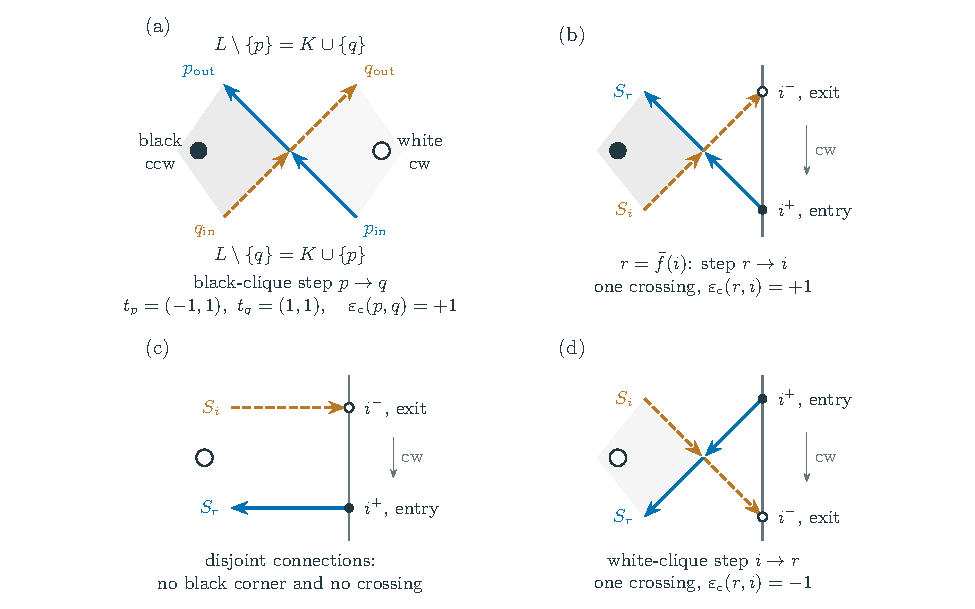
\includegraphics[width=\linewidth]{figures/clh_strand_corner.pdf}
\caption{The local sign count behind \eqref{eq:signed-excess}. (a)~An interior crossing at a black corner, with the
black, counterclockwise strand face to the west: the rays in clockwise order are $p_{\rm out},q_{\rm out},p_{\rm in},
q_{\rm in}$, the faces north and south are labelled $L\setminus\{p\}$ and $L\setminus\{q\}$, and the clique step
$p\to q$ has sign $\varepsilon_c(p,q)=+1$. (b)~The black resolution at a boundary position $i$ next to a black
vertex, with the exit $i^-$ before the entry $i^+$ clockwise: one crossing, the step $r\to i$, $r=\ba(i)$. (c)~Next
to a white vertex: no crossing. (d)~The other refinement, which is not used: it puts the entry first and gives the
white-clique step $i\to r$ with the opposite sign. Schematic.}
\label{fig:clh-strand-corner}
\end{figure}


\emph{Integral cancellation.}  First delete every bigon, cancelling its two
opposite occurrences.  Suppose occurrences of $p\to q$ and $q\to p$ remain.
They have distinct owner cycles: a winding-one cycle is vertex-simple by
Lemma~\ref{lem:winding-simple}, and a vertex-simple cycle containing both
orientations is precisely the already deleted bigon.

Remove $p\to q$ from its owner $C_1$ and $q\to p$ from its owner $C_2$.  The
remainders are paths
\[
   P_1:q\rightsquigarrow p,
   \qquad P_2:p\rightsquigarrow q.
\]
If $d=\operatorname{adv}(p,q)$, their advances are $n-d$ and $d$.
Consequently $P_1P_2$ is a closed walk of total advance $n$, hence a
vertex-simple winding-one cycle by Lemma~\ref{lem:winding-simple}.  Replace $C_1,C_2$ by
this cycle.  Each operation removes two edge occurrences, preserves every
signed multiplicity in \eqref{eq:signed-excess}, and therefore terminates.

At termination only one orientation of each unordered pair remains.
Equation~\eqref{eq:signed-excess} then forces exactly one occurrence of every
positive crossing edge and no occurrence of a noncrossing edge.  The surviving
winding-one cycles are edge-disjoint and exhaust $G_f^{\,x}$.  No bigon survives,
so every cycle has length at least three.
For the count, $\operatorname{adv}(p,q)=q-p+n\mathbf1_{p>q}$.
Summing around a winding-one cycle cancels the raw differences, so that cycle
contains exactly one wrapped edge. Summing over the partition gives
\eqref{eq:wp-cycle-count}.
\end{proof}

\begin{remark}[what the strand-diagram proof imports, and why nothing depends on it]\label{rem:wp-imports}
The proof just given rests on three imported facts --- the existence of a reduced alternating strand
diagram with prescribed strand permutation and the merge of the boundary vertex pairs
\cite[Lem.~14.6, Cor.~14.7 with Cor.~14.2; the map $T\mapsto D$ following Def.~14.3, and Lem.~14.4]{Postnikov},
and the clockwise orientation of the black-clique
vertices \cite[Rem.~9.6, with Thm.~9.12 and the two remarks after it]{OPS} --- and on the local sign
bookkeeping \eqref{eq:signed-excess}, which is derived above ray by ray, at interior corners and in the
boundary collars. The pointers into
\cite{Postnikov} have been checked against arXiv:math/0609764 (single version, no journal counterpart);
the black boundary resolution used above is not stated by that merge, whose map puts each entry before its
exit; it is the additional local construction given in the boundary collars of the proof. The \cite{OPS}
pointers have been checked. A reader who prefers not
to take those on trust can rely on the proof in \S\ref{sec:wp-combinatorial-bridge}: it proves the same
statement from the refined endpoint order alone, uses none of these citations, and is the version that is
machine checked (Remark~\ref{rem:machine}). Nothing later in the paper depends on which of the two proofs is
used.
\end{remark}

\subsection{The cotangent cycle inequality}
\begin{lemma}\label{lem:cot}
Let $\alpha_1,\dots,\alpha_m$ be positive angles with $m\ge3$ and $\sum\alpha_i=\pi$, and let
$d_1,\dots,d_m\in\R$ with $\sum d_i=0$. Then $\sum_i\cot(\alpha_i)\,d_i^2\ge0$, with equality iff all $d_i=0$.
\end{lemma}

\begin{proof}
At most one $\alpha_i$ exceeds $\pi/2$ (two would sum to $>\pi$). Suppose first that all
$\alpha_i\le\pi/2$. At most one of them equals $\pi/2$: two such angles would already sum to $\pi$,
leaving the remaining $m-2\ge1$ positive angles a sum of $0$. Every other cotangent is positive, so the
form is $\ge0$, and it vanishes only if $d_i=0$ whenever $\alpha_i<\pi/2$; the condition $\sum d_i=0$
then forces the remaining $d_i$, if there is one, to vanish as well. Otherwise let $\alpha_m>\pi/2$ and
$S=\pi-\alpha_m=\sum_{i<m}\alpha_i<\pi/2$. Weighted Cauchy--Schwarz gives
$\sum_{i<m}\cot(\alpha_i)d_i^2\ge(\sum_{i<m}d_i)^2/\sum_{i<m}\tan(\alpha_i)$, and strict superadditivity of
$\tan$ on $(0,\pi/2)$ (with all partial sums $\le S<\pi/2$) gives $\sum_{i<m}\tan\alpha_i<\tan S$. Using
$\sum_{i<m}d_i=-d_m$ and $\cot\alpha_m=-\cot S$,
\[
   \sum_i\cot(\alpha_i)d_i^2 > \frac{d_m^2}{\tan S}+\cot(\alpha_m)d_m^2 = \cot(S)d_m^2-\cot(S)d_m^2 = 0
\]
when $d_m\ne0$; if $d_m=0$ the positive terms force all $d_i=0$.
\end{proof}

\subsection{Positive semidefiniteness}
Figure~\ref{fig:clh-winding} sketches the argument of this subsection.

\begin{figure}[t]
\centering
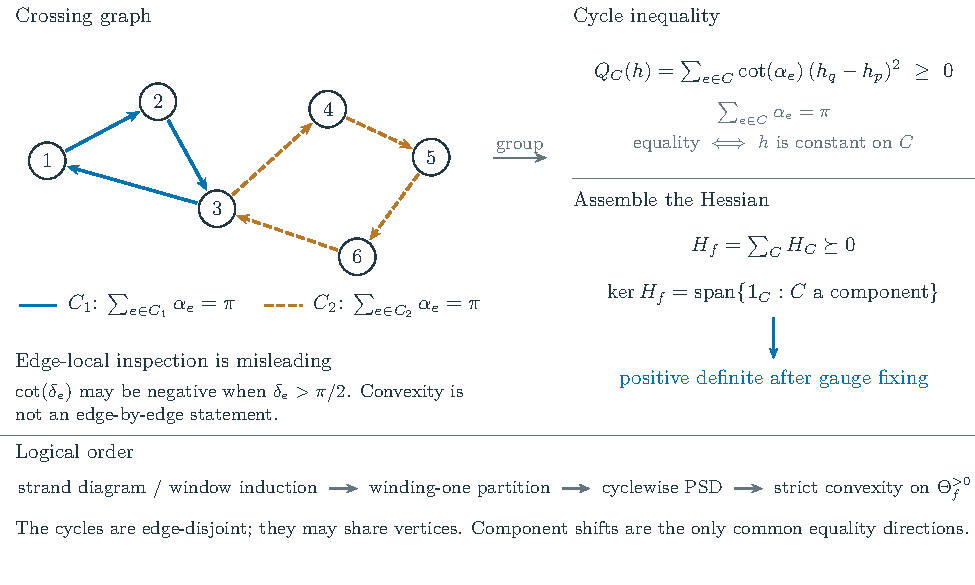
\includegraphics[width=\linewidth]{figures/clh_winding_cycle_hessian.pdf}
\caption{The directed crossing edges partition into edge-disjoint winding-one cycles. Individual cotangent weights may be negative, but each cycle quadratic form is positive semidefinite; their sum has exactly the crossing-component shifts as its kernel.}
\label{fig:clh-winding}
\end{figure}
\begin{proposition}\label{prop:psd}
For every $\theta\in\Theadm$, $H_f(\theta)\succeq0$ and
\[
\ker H_f(\theta)=\Span\{\mathbf1_C:C\text{ a component of }G_f^{\,x}\}.
\]
\end{proposition}

\begin{proof}
By Proposition~\ref{prop:wp} the edge set partitions into winding-one cycles; each edge appears in exactly
one, so \eqref{eq:hessian} gives, for every $h$,
\[
   h^{\mathsf T}H_f h=\sum_{\text{cycles }Z}\ \sum_{e=(p,q)\in Z}\cot(\delta_e(\theta))\,(h_q-h_p)^2.
\]
The angles $\delta_e$ are the lifted ones of \eqref{eq:delta-def}, positive on $\Theadm$ by
\eqref{eq:adm-delta}, and around each winding-one cycle they sum to $\pi$ by \eqref{eq:cycle-sum}.
The $h_q-h_p$ also sum to $0$ around the cycle. Thus Lemma~\ref{lem:cot} makes each inner sum $\ge0$, with equality
iff $h$ is constant along every edge of $Z$. Hence $H_f\succeq0$, and $h\in\ker H_f$ iff $h$ is constant along every crossing
edge, i.e.\ constant on each connected component.
\end{proof}

Figure~\ref{fig:clh-lean-hessian} shows, at the worked example, the form $h^{\mathsf T}H_fh$ on a plane tangent to the gauge slice and $\Psi_f$ along a segment of the slice.

\begin{figure}[htbp]
\centering
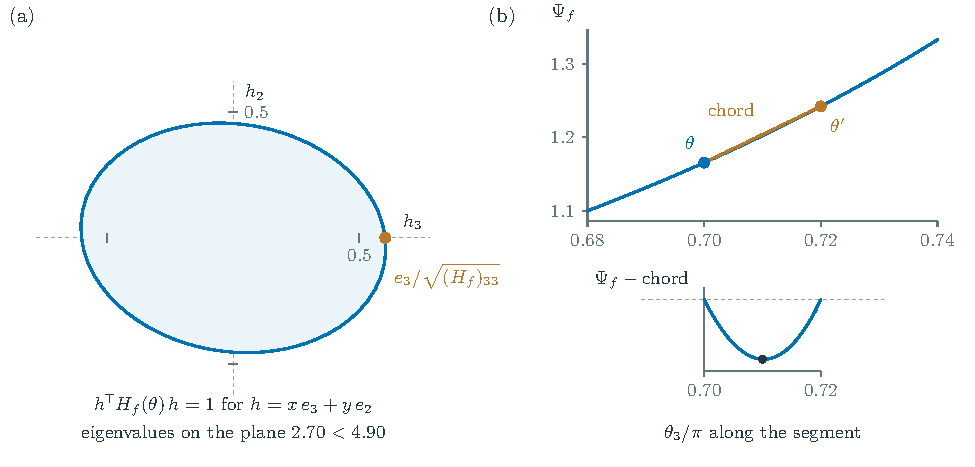
\includegraphics[width=\linewidth]{figures/clh_lean_hessian.pdf}
\caption{Worked example $\ba=(3,5,1,2,4)$, $\theta/\pi=(0,0.1,0.7,0.3,0.8)$. (a)~The curve $h^{\mathsf T}H_f(\theta)h=1$ for $h=x\,e_3+y\,e_2$, an ellipse: $H_f(\theta)$ is positive definite on directions with $h_1=0$ (Proposition~\ref{prop:psd}). (b)~$\Psi_f$, with $L(u)=\int_{\pi/2}^{u}\log\sin t\,dt$, along $\theta+\pi s\,e_3$ with its chord from $\theta$ to $\theta'=\theta+0.02\pi\,e_3$, and below it $\Psi_f$ minus the chord. Numerical values, in floating point.}
\label{fig:clh-lean-hessian}
\end{figure}

\subsection{The sharp convexity modulus away from the angular walls}
\label{sec:sharp-convexity}

The kernel theorem admits a sharp quantitative strengthening.  For $m\geq3$
and $0<\eta\leq\pi/m$, define
\begin{equation}\label{eq:sharp-kappa}
 \kappa_m^\star(\eta)
 :=\frac{\cot\eta-(m-1)\cot((m-1)\eta)}{m}.
\end{equation}
This number is positive.  Indeed, if $(m-1)\eta\geq\pi/2$, the second
cotangent is nonpositive; otherwise strict superadditivity of tangent gives
$(m-1)\tan\eta<\tan((m-1)\eta)$.

We first record a diagonal-form criterion.  If real numbers
$a_1,\ldots,a_m$ have at most one nonpositive entry, then
\begin{equation}\label{eq:diag-criterion}
 \sum_i a_i d_i^2\geq0\qquad\text{whenever }\sum_i d_i=0
\end{equation}
if and only if either every $a_i\geq0$, or exactly one entry, say $a_m$, is
negative, the others are positive, and
\begin{equation}\label{eq:reciprocal-criterion}
 \sum_i\frac1{a_i}\leq0.
\end{equation}
For in the latter case, putting $T=\sum_{i<m}a_i^{-1}$, weighted
Cauchy--Schwarz gives
\[
 \sum_{i<m}a_i d_i^2\geq\frac{d_m^2}{T}.
\]
Condition \eqref{eq:reciprocal-criterion} says $T\leq-1/a_m$, so
$1/T+a_m\geq0$.  Conversely, if
\eqref{eq:reciprocal-criterion} fails, take $d_m=-1$ and
$d_i=(1/a_i)/T$ for $i<m$.  Then $\sum_i d_i=0$ and the form equals
$1/T+a_m<0$.

\begin{lemma}[Localization of the shifted sign change]
\label{lem:sharp-localization}
Let $m\geq3$ and $0<\eta<\pi/m$, and put $c=\kappa_m^\star(\eta)$.  Then
\begin{equation}\label{eq:sharp-localization}
 0<c<\tan\!\left(\frac{(m-2)\eta}{2}\right).
\end{equation}
The upper bound fails at the excluded endpoint: $\kappa_m^\star(\pi/m)=\cot(\pi/m)
=\tan\bigl((m-2)(\pi/m)/2\bigr)$, so there the inequality is an equality.  This is harmless, because
Theorem~\ref{thm:sharp-cot} disposes of $\eta=\pi/m$ in its first sentence and invokes the lemma only for
$\eta<\pi/m$.
\end{lemma}

\begin{proof}
Only the upper bound remains after the positivity observation above.  Put
\[
 a=\frac{m\eta}{2},\qquad u=\frac{(m-2)\eta}{2},
 \qquad g(t)=t\cot t.
\]
Then $0<u<a<\pi/2$, $\eta=a-u$, $(m-1)\eta=a+u$, and
\begin{equation}\label{eq:g-difference}
 c=\frac{g(a-u)-g(a+u)}{2a}.
\end{equation}
Product-to-sum gives
\[
 g(a-u)-g(a+u)
 =\frac{a\sin(2u)-u\sin(2a)}{\sin^2a-\sin^2u}.
\]
The function $\tan t/t$ is strictly increasing on $(0,\pi/2)$, since its
derivative has the sign of $t-\sin t\cos t$, whose derivative is
$2\sin^2t$.  Hence
$u\sin a\cos u-a\sin u\cos a>0$, and a common-denominator calculation yields
\begin{align*}
 2a\tan u-[g(a-u)-g(a+u)]
 ={}&\frac{2\cos a}{\cos u(\sin^2a-\sin^2u)}\\
 &\qquad\cdot
 (u\sin a\cos u-a\sin u\cos a)>0.
\end{align*}
Now use \eqref{eq:g-difference}.
\end{proof}

\begin{theorem}[Sharp cotangent cycle inequality]
\label{thm:sharp-cot}
Let $m\geq3$, $0<\eta\leq\pi/m$, and
$\alpha_1,\ldots,\alpha_m\geq\eta$ with $\sum_i\alpha_i=\pi$.  If
$\sum_i d_i=0$, then
\begin{equation}\label{eq:sharp-cycle-bound}
 \sum_i\cot(\alpha_i)d_i^2
 \geq\kappa_m^\star(\eta)\sum_i d_i^2.
\end{equation}
The constant is best possible: the angle--velocity pair
\begin{equation}\label{eq:sharp-extremizer}
 \begin{aligned}
  (\alpha_1,\ldots,\alpha_m)
  &=(\eta,\ldots,\eta,\pi-(m-1)\eta),\\
  (d_1,\ldots,d_m)&=(1,\ldots,1,-(m-1))
 \end{aligned}
\end{equation}
attains equality, as do simultaneous permutations and nonzero scalar
multiples of the displayed velocity.
\end{theorem}

Figure~\ref{fig:clh-lean-sharp} shows the extremal pair~\eqref{eq:sharp-extremizer} for two choices of $(\eta,m)$.

\begin{figure}[htbp]
\centering
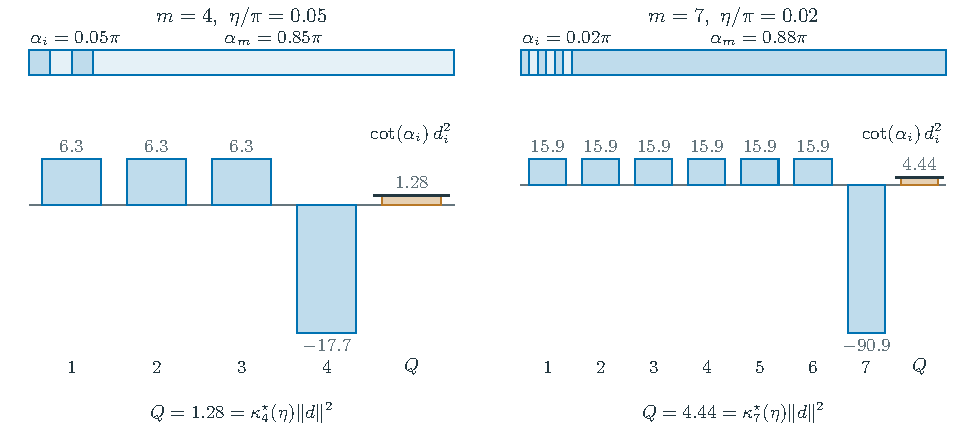
\includegraphics[width=\linewidth]{figures/clh_lean_sharp.pdf}
\caption{The extremal pair~\eqref{eq:sharp-extremizer} of Theorem~\ref{thm:sharp-cot} for $(\eta/\pi,m)=(0.05,4)$ (left) and $(0.02,7)$ (right). Above, the angles $\alpha_i$ stacked to $\pi$; below, the terms $\cot(\alpha_i)\,d_i^{2}$ and their sum $Q$, which equals $\kappa_m^\star(\eta)\sum_i d_i^2$ (the line on the last bar). Numerical values, in floating point.}
\label{fig:clh-lean-sharp}
\end{figure}

\begin{proof}
If $\eta=\pi/m$, the angle constraints force every $\alpha_i=\eta$, while
\eqref{eq:sharp-kappa} reduces to
$\kappa_m^\star(\eta)=\cot\eta$; the assertion and sharpness are immediate.
Assume henceforth that $0<\eta<\pi/m$.

Put $c=\kappa_m^\star(\eta)$, $\phi=\arctan c$, and
$\vartheta=\pi/2-\phi$, so that $\cot\vartheta=c$.  By
Lemma~\ref{lem:sharp-localization},
\begin{equation}\label{eq:phi-bound}
 0<\phi<\frac{(m-2)\eta}{2},
 \qquad
 \vartheta>\frac{\pi-(m-2)\eta}{2}.
\end{equation}
The shifted coefficient $A_i:=\cot\alpha_i-c$ is nonpositive exactly when
$\alpha_i\geq\vartheta$.  There cannot be two such angles, since then
\[
 \sum_i\alpha_i\geq2\vartheta+(m-2)\eta>\pi.
\]
If every $A_i\geq0$, the result follows; this includes the case in which
an angle equals $\vartheta$ (there is at most one with $\alpha_i\geq\vartheta$), so
that its $A_i=0$.  Suppose therefore that, after relabeling, $A_m<0$ and $A_i>0$
for $i<m$.  Then $\alpha_m>\vartheta$, hence $\cot\alpha_m-c\neq0$ and
$h(\pi-S)$ below is defined throughout the region considered.

Write $r=m-1$, $\beta_i=\alpha_i$ for $i<m$,
$S=\sum_{i<m}\beta_i$, and define
\[
 h(t)=\frac1{\cot t-c},\qquad
 F(\beta_1,\ldots,\beta_r)
 =\sum_{i<m}h(\beta_i)+h(\pi-S).
\]
Thus $F=\sum_iA_i^{-1}$.  We show that $F$ is nonincreasing in each
$\beta_i$ throughout the one-negative region.  Since
\[
 h'(t)=\frac1{(\cos t-c\sin t)^2}
 =\frac{\sec^2(t+\phi)}{1+c^2},
\]
one has
\begin{equation}\label{eq:F-sharp-derivative}
 \frac{\partial F}{\partial\beta_i}
 =h'(\beta_i)-h'(\alpha_m).
\end{equation}
Both $\beta_i+\phi$ and
$S-\phi=\pi-(\alpha_m+\phi)$ lie in $(0,\pi/2)$.  Moreover,
\[
 (S-\phi)-(\beta_i+\phi)
 =\sum_{j\neq i,m}\beta_j-2\phi
 \geq(m-2)\eta-2\phi>0.
\]
Since $\sec^2$ increases on $(0,\pi/2)$ and
$\sec^2(\alpha_m+\phi)=\sec^2(S-\phi)$,
\eqref{eq:F-sharp-derivative} is negative.

Set $P=\cot\eta$ and $Q=\cot((m-1)\eta)$.  At the boundary
configuration,
\[
 c=\frac{P-(m-1)Q}{m},\qquad
 P-c=\frac{(m-1)(P+Q)}m,\qquad
 -Q-c=-\frac{P+Q}{m}.
\]
Here
\[
 P+Q=\frac{\sin(m\eta)}{\sin\eta\sin((m-1)\eta)}>0,
\]
so the boundary point indeed lies in the one-negative region, and
\[
 F(\eta,\ldots,\eta)
 =\frac{m}{P+Q}-\frac{m}{P+Q}=0.
\]
Starting at this boundary point and increasing the coordinates one at a time
stays in the same one-negative region, with no change of the distinguished
index \(m\). At every intermediate point,
\(\eta\leq\beta_i\leq\beta_i^{\rm final}<\vartheta\), while
\(\alpha_m=\pi-\sum_{i<m}\beta_i\) decreases monotonically but remains at
least its final value \(\alpha_m^{\rm final}>\vartheta\). Thus \(A_m<0\)
and every \(A_i>0\) for \(i<m\) throughout the path. Therefore
\begin{equation}\label{eq:F-boundary-max}
 F(\beta_1,\ldots,\beta_r)\leq F(\eta,\ldots,\eta)=0.
\end{equation}
Thus \eqref{eq:reciprocal-criterion} holds.  Applying the diagonal criterion
to $A_i=\cot\alpha_i-c$ proves \eqref{eq:sharp-cycle-bound}.

For the data \eqref{eq:sharp-extremizer}, the shifted quadratic form equals
\[
 (m-1)\frac{(m-1)(P+Q)}m
 +(m-1)^2\left(-\frac{P+Q}{m}\right)=0.
\]
Hence the Rayleigh quotient is exactly $c$, proving sharpness.
\end{proof}

Fix a winding-one partition $\mathcal Z_f$ and set
\[
 \kappa_{f,\mathcal Z}^\star(\eta)
 :=\min_{Z\in\mathcal Z_f}\kappa_{|Z|}^\star(\eta),
 \qquad L_f^{\rm graph}:=BB^{\mathsf T}.
\]

\begin{corollary}[Sharp cyclewise Laplacian sandwich]
\label{cor:sharp-laplacian-sandwich}
Suppose $E_f\neq\varnothing$. If $\delta_e(\theta)\geq\eta$ for every crossing edge and
$\eta\leq\pi/|Z|$ for every $Z\in\mathcal Z_f$, then
\begin{equation}\label{eq:sharp-laplacian-sandwich}
 \kappa_{f,\mathcal Z}^\star(\eta)L_f^{\rm graph}
 \preceq H_f(\theta)
 \preceq\cot(\eta)L_f^{\rm graph}.
\end{equation}
If $\lambda_f^+$ is the smallest positive eigenvalue of
$L_f^{\rm graph}$, then on any convex set of admissible angles on which
every crossing angle is at least $\eta$ the
inverse of the component-shift quotient of $G_f$ satisfies
\begin{equation}\label{eq:sharp-inverse-lipschitz}
 \|[\theta]-[\theta']\|_{\rm quot}
 \leq
 \frac{\|G_f(\theta)-G_f(\theta')\|_2}
 {\kappa_{f,\mathcal Z}^\star(\eta)\lambda_f^+}.
\end{equation}
Here the target norm is the Euclidean norm in the explicit logarithmic
necklace-gradient coordinates, and $\|[x]\|_{\rm quot}$ is the Euclidean
distance from $x$ to the space of component shifts.
\end{corollary}

\begin{proof}
On each winding-one cycle the lifted angles sum to $\pi$ and the edge
differences sum to zero.  Sum Theorem~\ref{thm:sharp-cot} over the
edge-disjoint partition.  The upper bound follows from
\[
 \cot(\eta)L_f^{\rm graph}-H_f
 =B\operatorname{diag}(\cot\eta-\cot\delta_e)B^{\mathsf T}\succeq0.
\]
For the inverse estimate, choose the minimum-norm representative of
$[\theta']-[\theta]$, integrate the Hessian lower bound along the joining
segment, and apply Cauchy--Schwarz.  This gives strong monotonicity with
constant $\kappa_{f,\mathcal Z}^\star(\eta)\lambda_f^+$ and hence
\eqref{eq:sharp-inverse-lipschitz}.
\end{proof}

\begin{remark}[Meaning of sharpness]
\label{rem:sharp-cycle-scope}
Theorem~\ref{thm:sharp-cot} is sharp for a single cycle of fixed length.
The corollary takes the minimum over the cycles in one chosen winding-one
partition.  It does not claim that this minimum is the optimal coercivity
constant of the full Hessian when cycles share vertices or when a different
winding-one partition is chosen.  The metric statement remains confined to
the explicit logarithmic necklace-gradient coordinates; it is not a
raw-Pl\"ucker or intrinsic-Grassmannian bi-Lipschitz theorem.
\end{remark}

\section{The homeomorphism}\label{sec:homeo}

\begin{proof}[Proof of Theorem~\ref{thm:main}]
Let $f$ be loopless; no fixed-point-free hypothesis is needed, since
Propositions~\ref{prop:rowdiff}, \ref{prop:grad}, \ref{prop:wp} and \ref{prop:psd} are proved for every
loopless $f$ (Remark~\ref{rem:no-fpf}). Readers who prefer the component route may instead invoke
Lemma~\ref{lem:reduction}, whose commuting square \eqref{eq:reduction-square} reduces the statement to
the fixed-point-free factors; the argument below does not use it.

By \eqref{eq:adm-delta} the ambient admissible chamber is $\Theadm=\{0<\delta_e<\pi\}$, an open convex
polyhedron (each $\delta_e$ is an \emph{affine} function of $\theta$ by \eqref{eq:delta-def}, with
gradient \eqref{eq:delta-increment}); it is unbounded, being invariant under the global shift. The gauge
slice $\Thef\subseteq\Theadm$ (one angle fixed per crossing component) is an open convex polytope of
dimension $d_f=n-c_f$: within a component any two labels are joined by a path of crossing edges, and on
each winding-one cycle the $\delta_e$ are positive and sum to $\pi$ by \eqref{eq:cycle-sum}, which bounds
them; the angles of a singleton component are fixed outright by the gauge. Openness is meant in the
affine hull, and it is what the inverse-function and invariance-of-domain steps below need: $\Theadm$ is
open in $\R^n$, being cut out by finitely many strict affine inequalities, so
$\Thef=\Theadm\cap V$, with $V=\{\theta:\theta_{p_1}=\cdots=\theta_{p_{c_f}}=0\}$ an affine subspace of
dimension $n-c_f$, is open in $V$; and $\Thef$ is nonempty, because $\theta_j=\pi j/n$ satisfies every
inequality $\theta_p<\theta_q<\theta_p+\pi$ with $p<q$ and component shifts move it into the slice. So
$V$ is the affine hull of $\Thef$ (Galashin records the same fact after \cite[eq.~(4.3)]{Galashin},
identifying $\Thef$ with the interior of a $d_f$-dimensional polytope). By Proposition~\ref{prop:psd},
$\ker H_f=\Span\{\mathbf1_C\}$ is exactly the gauge directions, so $H_f\big|_{\Thef}\succ0$ everywhere on
$\Thef$: $\Psi_f\big|_{\Thef}$ is strictly convex.

\emph{Surjectivity.} By \eqref{eq:gauge-surjectivity}, $\Meas_f(\Thef)=\Meas_f(\Theadm)=\Critf$: every
admissible $\theta$ is carried into the slice by component shifts, which change neither the $\delta_e$
(both labels of a crossing lie in one component of $G_f^{\,x}$, so no crossing joins distinct components
and $\Theadm$ is shift-invariant) nor the value of $\Meas_f$
\cite[Prop.~4.2 and the paragraph following it]{Galashin}. Hence $\Meas_f\big|_{\Thef}$ is onto $\Critf$.
This is the one place where the theorem uses an input beyond the machinery of
\S\ref{sec:gradient}--\S\ref{sec:convex}: the present paper's coordinates give gauge-invariance of $G_f$,
which does not by itself give gauge-invariance of $\Meas_f$, because $R_f$ is not claimed injective.

\emph{Injectivity.} For $\theta,\theta'\in\Thef$ with $h=\theta'-\theta$,
$h^{\mathsf T}(G_f(\theta')-G_f(\theta))=\int_0^1 h^{\mathsf T}H_f(\theta+th)h\,dt>0$ unless $h=0$; so
$G_f\big|_{\Thef}$ is injective. Since $R_f\circ\Meas_f=G_f$, equal measurements have equal $G_f$, hence
equal $\theta$ in $\Thef$: $\Meas_f$ is injective on $\Thef$.

\emph{Homeomorphism.} $\Psi_f\big|_{\Thef}$ strictly convex with nonsingular Hessian makes
$G_f\big|_{\Thef}$ a local diffeomorphism (inverse function theorem) between the Euclidean spaces $\Thef$
and $\im(B)$ ($\dim\Thef=\dim\im(B)=d_f$, and $\im H_f=\im(B)$ because $\ker H_f=\ker B^{\mathsf T}$);
being globally injective, it is a homeomorphism onto its
open image, with continuous inverse $G_f^{-1}$. The invariance-of-domain step is applied \emph{only}
between the known Euclidean spaces $\Thef$ and $\im(B)$, never to the critical image. Now $R_f$ is
continuous on $\Critf$ and $R_f(\Critf)=\im(G_f\big|_{\Thef})\subseteq\operatorname{dom}(G_f^{-1})$, so
\[
   \Meas_f^{-1}=G_f^{-1}\circ R_f
\]
is a continuous inverse to $\Meas_f\big|_{\Thef}$, which is a continuous bijection onto $\Critf$ by the
injectivity and surjectivity steps. Hence $\Meas_f\colon\Thef\to\Critf$ is a homeomorphism, and the
inverse is the displayed explicit composition.

Figure~\ref{fig:clh-lean-slice-map} shows $G_f$ on one plane of the gauge slice at the worked example.

\begin{figure}[htbp]
\centering
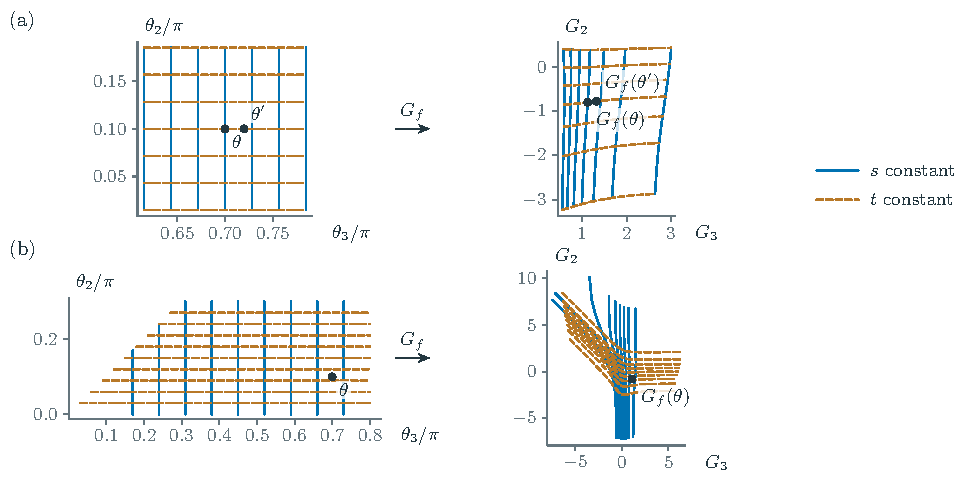
\includegraphics[width=\linewidth]{figures/clh_lean_slice_map.pdf}
\caption{The plane $\theta+\pi(s\,e_3+t\,e_2)$ of the gauge slice and its image under $G_f$, drawn in the components $(G_3,G_2)$, which is the gradient of the restriction of $\Psi_f$ to the plane, for $\ba=(3,5,1,2,4)$ and $\theta/\pi=(0,0.1,0.7,0.3,0.8)$. (a)~A grid near $\theta$ and the points $\theta$, $\theta'=\theta+0.02\pi\,e_3$ with their images; the image grid does not fold. (b)~Lines across the whole admissible part of the plane; their images run off where a gap $\delta_e$ reaches $0$ or $\pi$. Numerical values, in floating point.}
\label{fig:clh-lean-slice-map}
\end{figure}

\emph{Variational inverse.} Write $T$ for the vector space parallel to the gauge slice,
and fix $X\in\Critf$ and $y=R_f(X)$. The preimage $\theta_*\in\Thef$ just obtained
satisfies $G_f(\theta_*)=y$, so it is a stationary point of
$F_y(\theta)=\Psi_f(\theta)-\langle y,\theta\rangle$ on the slice. Strict convexity
makes it the unique global minimizer. Conversely, at a minimizer the first variation
gives $G_f(\theta)-y\in T^\perp$. This vector also belongs to $\im B$, and
$T^\perp\cap\im B=\{0\}$: a vector normal to the slice is supported on the one
fixed label of each component, whereas a vector in $\im B$ has sum zero on each
component. Thus $G_f(\theta)=y$, proving~\eqref{eq:variational-inverse}.
Existence here uses $y=R_f(X)$ with $X\in\Critf$; no existence claim for arbitrary
$y\in\im B$, or convergence guarantee for a numerical minimization algorithm, is needed.
By~\eqref{eq:lobachevsky}, the same minimizer uniquely maximizes
$\sum_e\Lambda(\delta_e(\theta))+\langle y,\theta\rangle$, the total cycle volume
plus the linear term.

\begin{figure}[htbp]
\centering
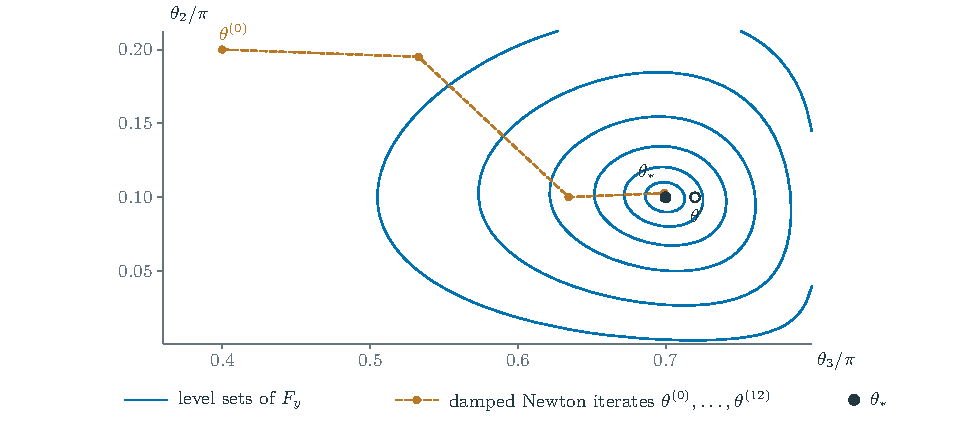
\includegraphics[width=\linewidth]{figures/clh_lean_inverse.pdf}
\caption{Level sets of $F_y=\Psi_f-\langle y,\cdot\rangle$ on the plane $\theta_*+\pi(s\,e_3+t\,e_2)$, for $\ba=(3,5,1,2,4)$, $\theta_*/\pi=(0,0.1,0.7,0.3,0.8)$ and $y=G_f(\theta_*)$; here $L(u)=\int_{\pi/2}^{u}\log\sin t\,dt$. Marked: the minimizer $\theta_*$, a competitor $\theta'=\theta_*+0.02\pi\,e_3$ with $F_y(\theta')>F_y(\theta_*)$, and twelve damped Newton steps in the gauge slice from $\theta^{(0)}/\pi=(0,0.2,0.4,0.6,0.8)$, projected to the plane, as an illustration with no convergence claim. Numerical values, in floating point.}
\label{fig:clh-lean-inverse}
\end{figure}

Figure~\ref{fig:clh-lean-inverse} shows the level sets of $F_y$ on one plane of the slice at the worked example.
\end{proof}

\begin{corollary}[inverting $G_f$ is minimizing]\label{cor:gradient-preimage}
For every $y\in G_f(\Thef)$ there is exactly one $\theta\in\Thef$ with $G_f(\theta)=y$, and it is the unique
minimizer of $F_y=\Psi_f-\langle y,\cdot\rangle$ on $\Thef$.
\end{corollary}

\begin{proof}
Write $y=G_f(\theta_0)$ with $\theta_0\in\Thef$. As in the paragraph \emph{Variational inverse} above, $\theta_0$
is a stationary point of $F_y$ on the gauge slice, so by strict convexity it is the unique minimizer of $F_y$ on
$\Thef$. Any $\theta\in\Thef$ with $G_f(\theta)=y$ equals $\theta_0$, because $G_f$ is injective on the gauge
slice, and any minimizer equals $\theta_0$ by uniqueness.
\end{proof}

The corollary restates the proof of Theorem~\ref{thm:main} from the side of $G_f$: computing the inverse of the
gradient at a point of its image is the same as minimizing $F_y$.



\begin{corollary}[the necklace coordinates determine the critical point]\label{cor:necklace-embedding}
For every loopless $f$ the map
\[
   N_f\colon\Critf\to\mathbb P^{n-1}_{>0},\qquad X\mapsto\bigl[\Delta_{I_1}(X):\cdots:\Delta_{I_n}(X)\bigr],
\]
is a topological embedding, with inverse $N\mapsto\Meas_f\bigl(G_f^{-1}(-P_fD\log N)\bigr)$ on its image,
where $\log$ is taken coordinatewise on any positive representative.
\end{corollary}

\begin{proof}
The necklace minors are continuous and positive on $\Critf\subseteq\Pi_f^{>0}$, so $N_f$ is continuous,
and $-P_fD\log N_f(X)=R_f(X)$ by \eqref{eq:untwisted}, independently of the representative. If
$N_f(X)=N_f(X')$, then $R_f(X)=R_f(X')$, and $X=X'$ because $\Meas_f^{-1}=G_f^{-1}\circ R_f$ by
Theorem~\ref{thm:main}. On the image of $N_f$ the displayed inverse is the composition of continuous maps
$-P_fD\log$, $G_f^{-1}$ (continuous on the open image of the slice, as in the proof of
Theorem~\ref{thm:main}) and $\Meas_f$.
\end{proof}

\begin{corollary}[Real-analytic critical coordinates]\label{cor:analytic-critical}
For every loopless bounded affine permutation $f$, including those with coloops,
the critical cell $\Critf$ is a real-analytic embedded submanifold of
$\Pi_f^\circ(\mathbb R)$, and hence of $\Gr(k,n)(\mathbb R)$, of dimension
$d_f=n-c_f$. The measurement map
\[
  \Meas_f:\Thef\longrightarrow\Critf
\]
is a real-analytic diffeomorphism, with inverse $G_f^{-1}\circ R_f$.
Its differential is injective on the tangent space
$T=\{h:h_{p_1}=\cdots=h_{p_{c_f}}=0\}$ at every point of $\Thef$.
The ordinary necklace map $N_f$ of Corollary~\ref{cor:necklace-embedding}
is also a real-analytic embedding into $\mathbb P^{n-1}_{>0}$.
All these assertions include admissible collisions of noncrossing labels.
\end{corollary}

\begin{proof}
We use the standard real-analytic structure on the real Grassmannian: on the
chart where a $k$-column minor is nonzero, a plane is represented uniquely by
a matrix whose corresponding columns form the identity matrix, and the
remaining entries are coordinates. Its transition maps are rational with
nonzero denominators. The open positroid variety is a smooth locally closed
algebraic subvariety defined over $\mathbb R$
\cite[Thm.~5.9]{KnutsonLamSpeyer}; its real locus has the induced
real-analytic submanifold structure. We do not assert smoothness of its
closure or of the complex critical variety.

The gauge slice is open in $T$, and has dimension $d_f$, as in the proof of
Theorem~\ref{thm:main}. The analytic map $\theta\mapsto(e^{i\theta_p})_p$
of \eqref{eq:t-of-theta} takes the whole slice into $\Theta_f^\circ$ of
\eqref{eq:theta-circ}. Composing with the regular map of
\cite[Prop.~5.1]{Galashin} is real-analytic, and
\cite[Lem.~5.13]{Galashin} and \eqref{eq:meas-identification} identify
this composition with $\Meas_f$. Its values are real. In the Grassmannian
charts just described, its coordinate functions are therefore real-valued
real-analytic functions, giving analyticity into the real Grassmannian.
Since the values lie in the smooth real locus of $\Pi_f^\circ$, the
same assertion holds with that target.

The left twist is regular on $\Pi_f^\circ$
\cite[\S5.4]{Galashin}, and its necklace minors do not vanish there
\cite[eq.~(2.4)]{Galashin}. After fixing projective scale locally,
$\log|\Delta_{I_r}(\widetilde\tau(X))|$ is real-analytic on the real
locus. Applying $P_fD$ removes the common scale. This gives a real-analytic
$\mathbb R^n$-valued extension of $R_f$ to a neighbourhood of $\Critf$.
Equivalently, use the ordinary-minor formula of Remark~\ref{rem:untwisted}.
Only its restriction to $\Critf$ needs to take values in $W:=\im(B)$.

By Proposition~\ref{prop:grad}, $G_f=B\log\sin\delta$ is real-analytic
on the admissible chamber, and the identity $R_f\circ\Meas_f=G_f$
holds on the whole slice. Thus, for $h\in T$,
\[
 dR_f|_{\Meas_f(\theta)}\,d\Meas_f|_\theta(h)=H_f(\theta)h.
\]
Here the differential of $R_f$ can be taken using the ambient extension.
Proposition~\ref{prop:psd} says that the kernel of $H_f$ consists exactly
of component shifts. Its intersection with $T$ is zero, so
$d\Meas_f|_\theta$ is injective on $T$. Theorem~\ref{thm:main} gives
that $\Meas_f$ is a homeomorphism onto its image with the subspace
topology. The analytic immersion theorem now makes this image an embedded
real-analytic submanifold of dimension $d_f$.

For the inverse, $H_f(\theta)$ has image $W$, and $H_f(\theta)|_T:T\to W$
is an isomorphism: it is injective and both spaces have dimension $d_f$.
This is an isomorphism between two possibly different subspaces of
$\mathbb R^n$, not an assertion that $H_f$ preserves $T$.
The analytic inverse function theorem therefore applies to
$G_f:\Thef\to W$. Its injectivity, established in the proof of
Theorem~\ref{thm:main}, makes the local analytic inverses agree on overlaps.
Consequently $G_f^{-1}$ is analytic on the open set $G_f(\Thef)\subset W$.
The restriction of $R_f$ to the embedded critical cell is analytic as a
$W$-valued map: one may compose its ambient extension with any linear
projection $\mathbb R^n\to W$. Its values belong to $G_f(\Thef)$, so
$\Meas_f^{-1}=G_f^{-1}\circ R_f$ is real-analytic.

Finally, $N_f$ is analytic into positive projective space. The well-defined
analytic map $\mathcal R([z])=-P_fD\log z$, for any positive representative $z$,
satisfies $\mathcal R\circ N_f\circ\Meas_f=G_f$. Differentiating shows that
$N_f\circ\Meas_f$ has injective differential, and therefore so does
$N_f$ on $\Critf$. Its topological embedding is
Corollary~\ref{cor:necklace-embedding}, so it is a real-analytic embedding.
Its inverse on its image is the analytic map
$N\mapsto\Meas_f(G_f^{-1}(-P_fD\log N))$.

There is no deleted collision locus in this argument. Equation~(5.2) of
\cite{Galashin} excludes $t_p=\pm t_q$ only for crossing pairs;
\cite[Prop.~5.1 and Lem.~5.13]{Galashin} apply at every admissible
specialization. The last paragraph of Proposition~\ref{prop:grad}
establishes the identity there directly. Noncrossing collisions are
interior points of the slice; crossing collisions are inadmissible and
are outside the statement. If $d_f=0$, the slice and critical cell are
single points, and the conclusions have their usual zero-dimensional
meaning.
\end{proof}

\begin{remark}[Independent measurement controls]\label{rem:top-cell-control}
Two finite numerical cross-checks of $R_f\circ\Meas_f=B\ell$ --- one against Galashin's independent
top-cell reconstruction \cite[\S9]{Galashin}, and one on every non-top loopless cell with $2\le n\le7$
--- are recorded in Appendix~\ref{app:lean-interface} (\emph{Finite checks}). They are not premises.
\end{remark}

\section{The all-rank critical Gr--OG shift}\label{sec:shift}

For $f=(3,5,6,7,9)$, Figure~\ref{fig:clh-lean-shift} shows $f$ beside its shift $f^\downarrow(p)=f(p-1)$.

\begin{figure}[htbp]
\centering
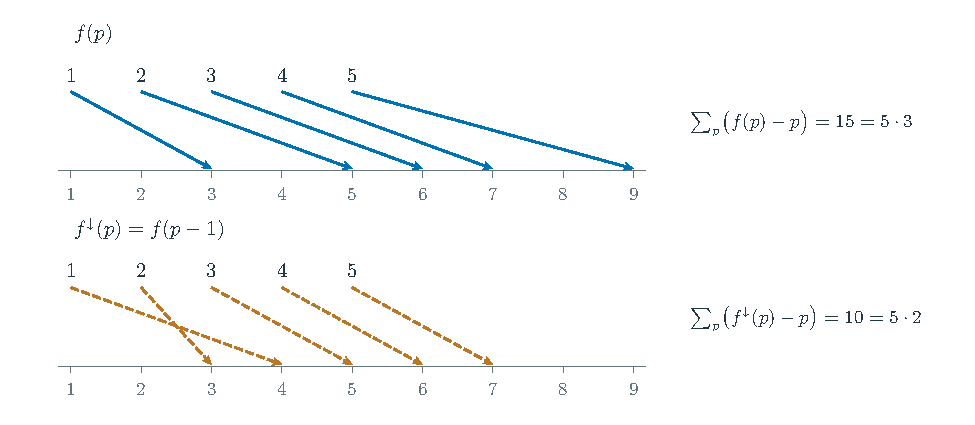
\includegraphics[width=\linewidth]{figures/clh_lean_shift.pdf}
\caption{The shift of the bounded affine permutation $f=(3,5,6,7,9)$, $\ba=(3,5,1,2,4)$, $n=5$. Top: $p\mapsto f(p)$. Bottom: $p\mapsto f^\downarrow(p)=f(p-1)$, where $f(0)=f(5)-5=4$. The displacement sums are $15=5\cdot3$ and $10=5\cdot2$, so the rank drops from $3$ to $2$. Evaluated by the formal definitions of Appendix~\ref{app:lean-interface}.}
\label{fig:clh-lean-shift}
\end{figure}

\begin{proof}[Proof of Corollary~\ref{cor:shift}]
Galashin observes that the reduced strand diagram of a loopless $f$ is the dual reduced strand diagram of
$f^\downarrow$; hence the $f$-admissible and dual $f^\downarrow$-admissible angle chambers are identified
by $\theta\mapsto\theta$ \cite[\S8.4]{Galashin}. Proposition~8.9 of \cite{Galashin} says that, if
Conjecture~4.3 holds for $f$, the dashed arrow in its Figure~24(b) is the composition of the three
homeomorphisms
\[
 \Crit_f^{>0}\xrightarrow{\ \Meas_f^{-1}\ }\Theta_f^{>0}
 \xrightarrow{\ \mathrm{id}\ }\widehat\Theta_{f^\downarrow}^{>0}
 \xrightarrow{\ \widehat\Meas_{f^\downarrow}\ }
 \widehat\Crit_{f^\downarrow}^{>0}.
\]
Theorem~\ref{thm:main} supplies the hypothesis for every loopless $f$ and gives
$\Meas_f^{-1}=G_f^{-1}\circ R_f$, proving the first assertion and its displayed constructive formula.
For $k=1$ the statement is degenerate but true: $f^\downarrow\in\mathcal B(0,n)$ and
$\Gr(0,n)$ is a point, so both sides are points and $\Phi_f$ is the unique map between them.

Now let $\tau$ be a matching on $[2N]$, and put
$f=f_\tau^{\mathrm{elec}}$ and $g=f_\tau^{\mathrm{Ising}}$.
The residue of $f^\downarrow(p)=f(p-1)$ is $\tau(p)$
\cite[\S7]{Galashin}. Moreover,
\[
 p\le f^\downarrow(p)=f(p-1)\le p+2N-1,
\]
so the shift is coloopless; it is also loopless because $\tau(p)\ne p$.
Uniqueness of the loopless bounded lift gives $f^\downarrow=g$.

We use the regular dual measurement of \cite[Remark~5.3]{Galashin}:
raw graph coordinates from (3.6) may have a common vanishing factor.
This map is invariant under translations on dual crossing components.
Indeed, put $h=\hat g$ and, for a dual $g$-admissible tuple $\varphi$,
set $\widetilde\psi=\widetilde\varphi\circ h^{-1}$, using affine
angle extensions. Proposition~3.4 of \cite{Galashin} gives
\[
 \widehat{\Meas}_g(\varphi)
 =\operatorname{alt}^{\perp}\bigl(\Meas_h(\psi)\bigr).
\]
The relabeling in that proposition sends a dual $g$-crossing component
$C$ to the ordinary $h$-crossing component $\bar h(C)$.
Translating $\varphi$ on $C$ therefore translates $\psi$ on $\bar h(C)$,
which preserves $\Meas_h$ by \cite[Proposition~4.2]{Galashin}.
The identity holds for the regular maps also where a raw graph vector
vanishes.

Let $\theta$ be $\tau$-admissible and let $\theta^0$ be its normalization
in the chosen gauge slice $\Theta_f^{>0}$. Proposition~7.2 of
\cite{Galashin} makes $\theta$ both $f$- and $g$-admissible, and
\S8.4 identifies the ordinary $f$-crossing components with the dual
$g$-crossing components. Thus ordinary gauge invariance and the dual
invariance just established give
\[
 \Phi_f\bigl(\Meas_f(\theta)\bigr)
 =\widehat{\Meas}_g(\theta^0)
 =\widehat{\Meas}_g(\theta)
 =\Meas_g(\theta).
\]
For the last equality, a boundary edge at $b_p$ of a black-boundary
representative of $g$ has strand label $\{p,\tau(p)\}$.
Its dual weight is $\sin(\pi/2)=1$ by $\tau$-isotropy, so (3.6)
and (1.2) agree on every edge. Theorem~7.3 of \cite{Galashin}
identifies the two ordinary measurements with the displayed embedded
response and correlation matrices. Consequently the restriction is
to the image of the $\tau$-admissible tuples in $\Crit_f^{>0}$;
the gauge representative $\theta^0$ need not itself be isotropic.
\end{proof}

\begin{remark}[what Corollary~\ref{cor:shift} is not]\label{rem:shift-scope}
Corollary~\ref{cor:shift} is a statement about \emph{critical} loci only. It is not an answer to
Question~9.2 of \cite{GalashinPylyavskyy}, which asks for a homeomorphism between the full electrical and
Ising spaces: for the top matching with $N\ge3$ the open electrical network cell has dimension
$\binom N2$, while the connected critical family has dimension $N-1$, and Proposition~8.9 of
\cite{Galashin} supplies nothing in the missing noncritical directions.
\end{remark}

\section*{A note on process}
Learned Response Labs is a research collaboration between the author and AI systems.
The proofs, text, software, atlases, and other artifacts of this program were primarily
generated by AI coding harnesses (OpenAI Codex and Anthropic Claude Code) operating
adversarially: results produced by one system were frozen, independently rederived,
and hostilely audited by the other before internal acceptance, with machine-checked
Lean~4/Mathlib components where noted. The author designed and directed the research
program --- the choice of problems, the harness and adversarial-audit architecture, and
the cross-domain references that shaped it. \par Before release, each paper is
reviewed internally in a \emph{reading edition}, which sets every formal statement
beside what checks it (a frozen Lean statement or a pinned exact certificate) and
every step without one beside its source; a release goes out only when every item
has been confirmed to say what the paper says. External review is pending, and
reviews received will be noted with the paper's public reading
edition.
\par The decision to circulate
this document, and the judgment that the process behind it makes the results worth a
referee's time, are the author's; the mathematics itself awaits external verification,
which is exactly what this document requests. Accordingly, the headline results are
offered as \emph{proof candidates pending external review}, and no claim in this document
should be treated as established until that review has occurred. This external-review
preprint is prepared for public circulation; it is not yet an arXiv version.

\begin{thebibliography}{99}
\setlength{\itemsep}{0pt}
\bibitem{Galashin} P.~Galashin, \emph{Critical varieties in the Grassmannian}, Comm.\ Math.\
  Phys.\ \textbf{401} (2023), no.~3, 3277--3333; arXiv:2102.13339v2.  Every locator cited here
  is the numbering of arXiv v2.
\bibitem{GuetzBoundary} A.~Guetz, \emph{Boundary compatibility of the critical Gr--OG shift, and exact
  finite atlases}, companion manuscript, in preparation.
\bibitem{GalashinPylyavskyy} P.~Galashin and P.~Pylyavskyy, \emph{The Ising model and the positive
  orthogonal Grassmannian}, Duke Math.\ J.\ \textbf{169} (2020), no.~10, 1877--1942; arXiv:1807.03282.
\bibitem{MullerSpeyer} G.~Muller and D.~E.~Speyer, \emph{The twist for positroid varieties}, Proc.\ Lond.\
  Math.\ Soc.\ (3) \textbf{115} (2017), no.~5, 1014--1071; arXiv:1606.08383v1.  The numbered
  results cited here are those of arXiv v1.
\bibitem{Postnikov} A.~Postnikov, \emph{Total positivity, Grassmannians, and networks}, arXiv:math/0609764 (2006).
\bibitem{KnutsonLamSpeyer} A.~Knutson, T.~Lam, and D.~E.~Speyer, \emph{Positroid varieties:
  juggling and geometry}, Compos.\ Math.\ \textbf{149} (2013), no.~10, 1710--1752.
\bibitem{OPS} S.~Oh, A.~Postnikov, and D.~E.~Speyer, \emph{Weak separation and plabic graphs},
  Proc.\ Lond.\ Math.\ Soc.\ (3) \textbf{110} (2015), no.~3, 721--754; arXiv:1109.4434.
\bibitem{Kenyon} R.~Kenyon, \emph{The Laplacian and Dirac operators on critical
  planar graphs}, Invent.\ Math.\ \textbf{150} (2002), 409--439;
  arXiv:math-ph/0202018v1 (titled \emph{The Laplacian and $\bar\partial$ operators
  on critical planar graphs}). The numbered statements cited here use arXiv v1.
\bibitem{KenyonSchlenker} R.~Kenyon and J.-M.~Schlenker, \emph{Rhombic embeddings of planar
  graphs with faces of degree 4}, arXiv:math-ph/0305057v1; published as
  \emph{Rhombic embeddings of planar quad-graphs}, Trans.\ Amer.\ Math.\ Soc.\
  \textbf{357} (2005), no.~9, 3443--3458. The theorem locator uses arXiv v1.
\bibitem{BoutillierCimasoniDeTiliere} C.~Boutillier, D.~Cimasoni, and
  B.~de~Tili\`ere, \emph{Isoradial immersions}, arXiv:1912.10297v4 (2021).
  The numbered statements cited here use arXiv v4.
% ---------------------------------------------------------------------------
% The seven entries Milnor through Pinkall--Polthier support only the
% "Relation to hyperbolic volume" subsection of Section 1; no theorem of this
% paper uses them.  All seven were checked against the sources on 2026-09-08
% (bibliographic data and the statement each is cited for).
% ---------------------------------------------------------------------------
\bibitem{Milnor} J.~Milnor, \emph{Hyperbolic geometry: the first 150 years},
  Bull.\ Amer.\ Math.\ Soc.\ (N.S.)\ \textbf{6} (1982), no.~1, 9--24; and
  W.~P.~Thurston, \emph{The geometry and topology of three-manifolds}, lecture notes,
  1979, ch.~7 (``Computation of volume'', by J.~Milnor).
\bibitem{Rivin1994} I.~Rivin, \emph{Euclidean structures on simplicial surfaces and hyperbolic volume},
  Ann.\ of Math.\ (2) \textbf{139} (1994), no.~3, 553--580.
\bibitem{Rivin1996} I.~Rivin, \emph{A characterization of ideal polyhedra in hyperbolic $3$-space},
  Ann.\ of Math.\ (2) \textbf{143} (1996), no.~1, 51--70.
\bibitem{FuterGueritaud} D.~Futer and F.~Gu\'eritaud, \emph{From angled triangulations to hyperbolic
  structures}, Contemp.\ Math.\ \textbf{541} (2011), 159--182; arXiv:1004.0440.
\bibitem{BobenkoSpringborn} A.~I.~Bobenko and B.~A.~Springborn, \emph{Variational principles for circle
  patterns and Koebe's theorem}, Trans.\ Amer.\ Math.\ Soc.\ \textbf{356} (2004), no.~2, 659--689;
  arXiv:math/0203250.
\bibitem{Duffin} R.~J.~Duffin, \emph{Distributed and lumped networks}, J.\ Math.\ Mech.\ \textbf{8}
  (1959), no.~5, 793--826.
\bibitem{PinkallPolthier} U.~Pinkall and K.~Polthier, \emph{Computing discrete minimal surfaces and
  their conjugates}, Experiment.\ Math.\ \textbf{2} (1993), no.~1, 15--36.
\bibitem{LamGrassmann} T.~Lam, \emph{Totally nonnegative Grassmannian and Grassmann polytopes}, lecture notes, Current Developments in Mathematics 2014; arXiv:1506.00603v1, whose numbering is cited.
\end{thebibliography}

\appendix
\section{Formal statements and their geometric interface}\label{app:lean-interface}

The formal source for this paper is written in Lean~\texttt{4.33.0-rc1} with Mathlib; the exact
Mathlib revision is recorded in its dependency lockfile, \texttt{lake-manifest.json}. The coloop-inclusive
source supplement (\SourceSupplementRef) includes a source manifest, that lockfile, the exact
declarations and their proof modules. Every theorem named in this appendix, except the auxiliary lemmas
marked as such, is also stated, without its proof, in one of fifteen frozen
statement files kept apart from the proofs: thirteen for the \texttt{Conj43.} statements, and two for the
\texttt{TP.} statements on loops and on decorated permutations, which come from a companion formal
library for totally positive combinatorics and are included in the supplement. The proofs are checked
against those frozen statements by
the Comparator tool for Lean, which compares each proved statement with its frozen copy, replays the
proofs in the Lean kernel, and admits only the axioms \texttt{propext}, \texttt{Classical.choice} and
\texttt{Quot.sound}. The displays below render the formal statements in mathematical notation. Lean does
not construct the measurement map: the conditional theorem at the end of this appendix takes the
properties of the measurement map that the proof of Theorem~\ref{thm:main} uses as hypotheses, and the
paragraph after it says what each hypothesis stands for.

\paragraph{Domain and crossing convention.}
\texttt{Conj43.\allowbreak LooplessBAP n} contains a permutation $\sigma$ of
$\{0,\ldots,n-1\}$. For $n>0$, its bounded lift is
$f(i)=i+1+((\sigma(\bar i)-i-1)\bmod n)$, with the periodic extension understood.
Thus a fixed point of $\sigma$ represents a coloop $f(i)=i+n$; it never
represents a loop. Add one to the Lean labels to obtain the paper's labels.
Writing $s_p=\sigma^{-1}(p)$, the resolved circle has modulus $5n$, entry
position $5s_p+4$ and exit position $5p+1$. The predicate
\texttt{Conj43.\allowbreak CrossEdge F p q} requires strict clockwise order
\[
 (5s_p+4,\;5s_q+4,\;5p+1,\;5q+1)\pmod{5n}.
\]
Here clockwise means that the four positive cyclic increments sum to $5n$.
This is the endpoint order $s_p^+,s_q^+,p^-,q^-$ used in \S\ref{sec:setup},
including the exit-before-entry convention at a shared label
(Lemma~\ref{lem:halfopen}(b)). The two Mis classes are read from the same positions, clockwise and
counterclockwise.
The crossing list enumerates this predicate on all ordered pairs, without
duplicates. The first necklace term is $\{x:x\le\sigma^{-1}(x)\}$; subsequent
terms remove the current label and insert its image. In particular a coloop
belongs to every necklace term. Lean row $r$ is the paper's row $I_{r+1}$.

\paragraph{The interface with Galashin's definitions.}
Lean also transcribes the definitions of \cite{Galashin}, in his labels $1,\ldots,n$: loopless bounded
affine permutations, the affine necklace formula $I_r=\{f(a)\bmod n: a<r\le f(a)\}$, the refined
boundary with its exit and entry points $x^-,x^+$ \cite[Def.~1.5]{Galashin}, affine $f$-crossings and
alignments, the classes $\mathrm{Mis}^{\uparrow\downarrow}$ and $\mathrm{Mis}^{\downarrow\uparrow}$
\cite[\S5.4]{Galashin}, and the exponent of \eqref{eq:gal512}. The affine $f$-crossing is transcribed
with $t=f^{-1}(q)$; the definition before \cite[eq.~(3.2)]{Galashin} prints $t:=f^{-1}(p)$, repeating the
first argument. Against these transcriptions:
\begin{itemize}
\item the bounded lift, with labels shifted by one, is a loopless bounded affine permutation of rank
between $1$ and $n$ whose residues are $\sigma$ shifted by one (\texttt{Conj43.\allowbreak galashin\_\allowbreak isLooplessBAP}, \texttt{Conj43.\allowbreak galashin\_\allowbreak rank\_\allowbreak range}, \texttt{Conj43.\allowbreak galashin\_\allowbreak residues}); the
encoding is injective and onto the loopless bounded affine permutations of every rank
(\texttt{Conj43.\allowbreak galashin\_\allowbreak injective}, \texttt{Conj43.\allowbreak galashin\_\allowbreak surjective}), never has a loop
(\texttt{Conj43.\allowbreak galashin\_\allowbreak no\_\allowbreak loops}), and makes a fixed point of $\sigma$ exactly a coloop
(\texttt{Conj43.\allowbreak galashin\_\allowbreak coloop});
\item Lean's necklace row $r$ is his $I_{r+1}$ (\texttt{Conj43.\allowbreak galashin\_\allowbreak necklace});
\item {\sloppy the positions $5s_p+4$ and $5p+1$ order any four refined points as his boundary does
(\texttt{Conj43.\allowbreak encode\_\allowbreak clockwise4}), parts (a)--(c) of Lemma~\ref{lem:halfopen} hold on his refined boundary
(\texttt{Conj43.\allowbreak halfopen\_\allowbreak a}, \texttt{Conj43.\allowbreak halfopen\_\allowbreak b}, \texttt{Conj43.\allowbreak halfopen\_\allowbreak L1}, \texttt{Conj43.\allowbreak halfopen\_\allowbreak L2}, \texttt{Conj43.\allowbreak halfopen\_\allowbreak L3}), and so does
\eqref{eq:arc} (\texttt{Conj43.\allowbreak necklace\_\allowbreak iff\_\allowbreak refinedArc});\par}
\item \texttt{Conj43.\allowbreak CrossEdge F p q} holds exactly when representatives of $p+1$ and $q+1$ form
his affine $f$-crossing (\texttt{Conj43.\allowbreak crossEdge\_\allowbreak iff\_\allowbreak affine}); two distinct labels are aligned in his sense
exactly when they are in no crossing and in neither Mis class (\texttt{Conj43.\allowbreak alignment\_\allowbreak iff\_\allowbreak affine}); the two
Mis predicates are his classes (\texttt{Conj43.\allowbreak misUD\_\allowbreak iff\_\allowbreak galashin}, \texttt{Conj43.\allowbreak misDU\_\allowbreak iff\_\allowbreak galashin}); two
strands cross in some direction exactly when their chords interleave on the circle
(\texttt{Conj43.\allowbreak crossEdge\_\allowbreak iff\_\allowbreak interleave}); and no label crosses itself, while two distinct
labels have four distinct refined endpoints (\texttt{Conj43.\allowbreak crossEdge\_\allowbreak irrefl},
\texttt{Conj43.\allowbreak chord\_\allowbreak endpoints\_\allowbreak distinct});
\item \texttt{Conj43.\allowbreak pairExponent} is the exponent of the pair in \eqref{eq:gal512} on the face label that his
necklace formula gives (\texttt{Conj43.\allowbreak pairExponent\_\allowbreak eq\_\allowbreak galashin}).
\end{itemize}

\paragraph{Cotangent inequality.}
\texttt{Conj43.\allowbreak cot\_\allowbreak cycle\_\allowbreak inequality} states, for $m\ge3$ and
$\alpha,d:\{0,\ldots,m-1\}\to\R$,
\[
 \left(\forall i,\ \alpha_i>0\right),\quad
 \sum_i\alpha_i=\pi,\quad\sum_i d_i=0
 \quad\Longrightarrow\quad
 \begin{cases}
  \sum_i\cot(\alpha_i)d_i^2\ge0,\\
  \sum_i\cot(\alpha_i)d_i^2=0\ \Longleftrightarrow\ \forall i,\ d_i=0.
 \end{cases}
\]

\paragraph{Row difference.}
\texttt{Conj43.\allowbreak rowdiff} states, for $n>0$ and $F:\texttt{LooplessBAP n}$,
\[
 \texttt{Pmat}\,F\;\texttt{Dmat}\,n\;\texttt{Mmat}\,F=\texttt{Bmat}\,F,
\]
an identity of integer matrices whose columns are the directed crossing edges, with
$B_{x,(p,q)}=\mathbf1_{x=q}-\mathbf1_{x=p}$, $(Dz)_r=z_{r+1}-z_r$ and $(Pz)_x=z_{s_x}$. The full form is
stated separately, with columns indexed, as in \S\ref{sec:mn}, by the unordered pairs $p<q$. There
$(M_N)_{r,\{p,q\}}$ is the exponent of the pair on necklace row $r$ read from \eqref{eq:gal512}
(\texttt{Conj43.\allowbreak pairExponent}: $+1$ for a $\mathrm{Mis}^{\uparrow\downarrow}$ pair on a row containing
both labels, $+1$ for a $\mathrm{Mis}^{\downarrow\uparrow}$ pair on a row containing neither, $-1$ for a
crossing $p\to q$ on a row containing $p$ but not $q$, and $0$ otherwise), and the column of $B$ is
$e_q-e_p$ if $p\to q$, $e_p-e_q$ if $q\to p$, and $0$ if the pair carries no crossing. For such a pair,
\texttt{Conj43.\allowbreak pairExponent\_\allowbreak nonCross} states that its exponent is $0$ on every necklace row and
\texttt{Conj43.\allowbreak full\_\allowbreak pair\_\allowbreak columns\_\allowbreak zero} that its column vanishes in $M_N$, in $P_fDM_N$ and in $B$;
\texttt{Conj43.\allowbreak rowdiff\_\allowbreak full\_\allowbreak pairs} states
\[
 P_f\,D\,M_N=B
\]
over all unordered pairs, which is Proposition~\ref{prop:rowdiff} as stated. The coloop facts of its
proof (a coloop crosses nothing, lies in every necklace row, and has zero rows in $B$ and in $P_fDM_N$)
are \texttt{Conj43.\allowbreak not\_\allowbreak crossEdge\_\allowbreak of\_\allowbreak coloop\_\allowbreak fst}, \texttt{Conj43.\allowbreak coloop\_\allowbreak mem\_\allowbreak necklace},
\texttt{Conj43.\allowbreak Bmat\_\allowbreak coloop\_\allowbreak row} and \texttt{Conj43.\allowbreak PDM\_\allowbreak coloop\_\allowbreak row}. In the encoding of the previous
paragraph, part (c) of Lemma~\ref{lem:halfopen} for labels that are not coloops is proved as the
auxiliary Lean lemmas \texttt{Conj43.\allowbreak arc\_\allowbreak L1}, \texttt{Conj43.\allowbreak arc\_\allowbreak L2} and \texttt{Conj43.\allowbreak arc\_\allowbreak L3}, and
equation~\eqref{eq:arc} by induction along the necklace recursion. The proof of
\texttt{Conj43.\allowbreak rowdiff} uses \texttt{Conj43.\allowbreak arc\_\allowbreak L3} and
equation~\eqref{eq:arc} for the crossing columns and \texttt{Conj43.\allowbreak inArcN\_\allowbreak indicator\_\allowbreak diff}, the boundary of a
half-open arc, for their row differences; the vanishing of the Mis columns uses
\texttt{Conj43.\allowbreak arc\_\allowbreak L1} and \texttt{Conj43.\allowbreak arc\_\allowbreak L2}. None of these auxiliary lemmas is among
the frozen statements.

\paragraph{Existence of a winding-one partition.}
\texttt{Conj43.\allowbreak winding\_\allowbreak one\_\allowbreak partition} states, for $F:\texttt{LooplessBAP n}$,
that there is a list of vertex lists $\mathcal C$ such that
\[
 \begin{gathered}
  \forall c\in\mathcal C,\quad |c|\ge3,\quad c\text{ has no repeated vertex},
       \quad\operatorname{winding}(c)=n,\\
  \mathop{\mathrm{concat}}_{c\in\mathcal C}\operatorname{cycleEdges}(c)
       \text{ is a permutation of }\operatorname{crossEdges}(F).
 \end{gathered}
\]
Here $\operatorname{cycleEdges}(c)$ pairs consecutive entries, including the
last with the first, and winding is the sum of $(q-p)\bmod n$ over those edges.
The permutation assertion gives both edge exhaustion and disjointness.
The auxiliary theorem \texttt{Conj43.\allowbreak crossEdges\_\allowbreak subset\_\allowbreak cover} supplies the
cover inclusion used in its proof. \texttt{Conj43.\allowbreak partition\_\allowbreak card} states that every such list $\mathcal C$ has as
many entries as there are wrapped crossing edges $(p,q)$, those with $q<p$, which is the second form of
\eqref{eq:wp-cycle-count}; it rests on \texttt{Conj43.\allowbreak winding\_\allowbreak eq\_\allowbreak wrapped}: a vertex list with no repeated
vertex winds $n$ times its number of wrapped edges. For the first form,
\texttt{Conj43.\allowbreak partition\_\allowbreak advance} states that $n|\mathcal C|$ is the total advance
$\sum_{(p,q)\in E_f}\operatorname{adv}(p,q)$ of the crossing edges, and
\texttt{Conj43.\allowbreak crossEdges\_\allowbreak advance} that this total is $n$ times the number of wrapped edges. For a decorated permutation, loops allowed,
\texttt{TP.\allowbreak decCrossEdge\_\allowbreak iff} and \texttt{TP.\allowbreak decCrossEdges\_\allowbreak eq} state that its crossing relation and its
crossing edges are those of the loopless lift of its
underlying permutation, and \texttt{TP.\allowbreak dec\_\allowbreak winding\_\allowbreak one\_\allowbreak partition} gives it the same
partition.

\paragraph{Notation for the analytic statements.}
Write $E_f$ for the directed crossing edges, $\delta_{pq}(\theta)=\theta_q-\theta_p+\pi\,\mathbf1[q<p]$
for $(p,q)\in E_f$ (equation~\eqref{eq:delta-def}), $\Theadm=\{\theta\in\R^n:0<\delta_e(\theta)<\pi
\text{ for all }e\in E_f\}$, $B$ the real incidence matrix with a column for each $e\in E_f$,
$\ell_e=\log\sin\delta_e$, $G=B\ell$,
\[
 Q_\theta(h)=\sum_{(p,q)\in E_f}\cot\delta_{pq}(\theta)\,(h_q-h_p)^2,\qquad
 \Psi(\theta)=\sum_{e\in E_f}\int_{\pi/2}^{\delta_e(\theta)}\log\sin t\,dt ;
\]
this $\Psi$ satisfies \eqref{eq:potential} and differs from any other antiderivative choice, such as
the normalization $L(0)=0$ of \S\ref{sec:intro}, by a constant. Two labels lie in the same component when a path of crossing edges, taken in either
direction, joins them. For $a\in\R^n$ the formal gauge slice is
\[
 S_a=\{\theta\in\Theadm:\ \theta_p=a_p\ \text{whenever $p$ is the least label of its component}\}.
\]
With $a=0$ this is Galashin's slice $\Thef$ \cite[eq.~(4.3)]{Galashin} for the representatives
$p_C=\min C$; another choice of representatives gives a slice carried onto this one by component
shifts, which change neither $\Meas_f$ nor $G_f$.

\paragraph{Cycle sums, the assembled Hessian and the hinge.}
For a vertex list $c$ of length at least $3$ with $\operatorname{winding}(c)=n$,
\texttt{Conj43.\allowbreak cycle\_\allowbreak wrap\_\allowbreak sum} states that exactly one edge of $c$ is wrapped, and, if $c$ has no
repeated vertex, \texttt{Conj43.\allowbreak delta\_\allowbreak cycle\_\allowbreak sum} states $\sum_{e\in c}\delta_e(\theta)=\pi$ for every
$\theta\in\R^n$, which is \eqref{eq:cycle-sum}. \texttt{Conj43.\allowbreak hessian\_\allowbreak matrix\_\allowbreak form} states
$h^{\mathsf T}B\operatorname{diag}(\cot\delta_e)B^{\mathsf T}h=Q_\theta(h)$, and for
$\theta\in\Theadm$, \texttt{Conj43.\allowbreak hessian\_\allowbreak psd}, \texttt{Conj43.\allowbreak hessian\_\allowbreak kernel\_\allowbreak components} and
\texttt{Conj43.\allowbreak hessian\_\allowbreak matrix\_\allowbreak kernel} state
\[
 Q_\theta(h)\ge0,\qquad
 Q_\theta(h)=0\iff B\operatorname{diag}(\cot\delta_e)B^{\mathsf T}h=0
 \iff h\text{ is constant on every component},
\]
which is Proposition~\ref{prop:psd}. For $\theta\in\Theadm$, $(p,q)\in E_f$ and $t_j=e^{i\theta_j}$,
\texttt{Conj43.\allowbreak hinge\_\allowbreak identity} states $\lvert[\![t_q,t_p]\!]_+\rvert=2\sin\delta_{pq}(\theta)$, with the
bracket of \eqref{eq:bracket-plus}, which is Lemma~\ref{lem:hinge}.

\paragraph{The potential, its gradient, and convexity on the slice.}
\texttt{Conj43.\allowbreak logSinPrimitive\_\allowbreak derivative} states
$\frac{d}{du}\int_{\pi/2}^{u}\log\sin t\,dt=\log\sin u$ for $0<u<\pi$, and
\texttt{Conj43.\allowbreak admissible\_\allowbreak isOpen} that $\Theadm$ is open in $\R^n$. At every $\theta\in\Theadm$,
\texttt{Conj43.\allowbreak potential\_\allowbreak gradient} states that $\Psi$ is differentiable with gradient $G(\theta)$, and
\texttt{Conj43.\allowbreak gradient\_\allowbreak hessian} that $G$ is differentiable with derivative
$B\operatorname{diag}(\cot\delta_e(\theta))B^{\mathsf T}$, both also as strict derivatives; this is the
calculus of Proposition~\ref{prop:grad}. \texttt{Conj43.\allowbreak incidence\_\allowbreak degree\_\allowbreak balance} states $B\mathbf1=0$,
\texttt{Conj43.\allowbreak gradient\_\allowbreak edge\_\allowbreak constant} states $B(\ell+c\mathbf1)=B\ell$, and
\texttt{Conj43.\allowbreak gradient\_\allowbreak component\_\allowbreak shifts} states $G(\theta+s)=G(\theta)$ for every $s$ constant on
components. For $\theta\in\Theadm$ and $h\ne0$ vanishing at the least label of every component,
\texttt{Conj43.\allowbreak hessian\_\allowbreak gauge\_\allowbreak positive} states $Q_\theta(h)>0$. For every $a\in\R^n$: $\Psi$ is strictly
convex on $S_a$ (\texttt{Conj43.\allowbreak potential\_\allowbreak slice\_\allowbreak strictConvex}); $\langle G(y)-G(x),y-x\rangle>0$ for
distinct $x,y\in S_a$ (\texttt{Conj43.\allowbreak gradient\_\allowbreak slice\_\allowbreak strictMonotone}), so $G$ is injective on $S_a$
(\texttt{Conj43.\allowbreak gradient\_\allowbreak slice\_\allowbreak injective}); $G|_{S_a}$ is a topological embedding into $\R^n$
(\texttt{Conj43.\allowbreak gradient\_\allowbreak slice\_\allowbreak embedding}) and an open embedding into $\im B$ with its subspace
topology (\texttt{Conj43.\allowbreak gradient\_\allowbreak incidence\_\allowbreak openEmbedding}); each $x\in S_a$ is the unique minimizer on
$S_a$ of $z\mapsto\Psi(z)-\langle G(x),z\rangle$ (\texttt{Conj43.\allowbreak potential\_\allowbreak variational\_\allowbreak inverse}); and
for every $y\in G(S_a)$ the function $z\mapsto\Psi(z)-\langle y,z\rangle$ has exactly one minimizer on
$S_a$ (\texttt{Conj43.\allowbreak variational\_\allowbreak image\_\allowbreak minimizer}); and that minimizer is the
gradient preimage: $y$ has exactly one preimage in $S_a$, and it is the minimizer
(\texttt{Conj43.\allowbreak variational\_\allowbreak gradient\_\allowbreak preimage}, a corollary of the two;
with $a=0$ it is Corollary~\ref{cor:gradient-preimage}). These are the convexity, injectivity,
homeomorphism and variational steps of the proof of Theorem~\ref{thm:main}. An earlier composition
theorem, \texttt{Conj43.\allowbreak measurement\_\allowbreak conditional\_\allowbreak homeomorphism}, assumes the assembled identity
$R\circ\mathrm{Meas}=G$; the theorem below derives that identity instead.

\paragraph{Necklace logarithms.}
Put $\lambda_{pq}(\theta)=\log\lvert[\![t_q,t_p]\!]_+\rvert$ for $p<q$, $t_j=e^{i\theta_j}$ (Lean's
logarithm is $0$ at $0$; every pair whose bracket can vanish on $\Theadm$ has coefficient $0$ below).
For every $\theta\in\R^n$, \texttt{Conj43.\allowbreak necklace\_\allowbreak log\_\allowbreak crossing} states that $M_N\lambda(\theta)$, summed
over all unordered pairs, equals the same sum over the crossing edges alone, so the Mis columns vanish on
necklace rows; \texttt{Conj43.\allowbreak necklace\_\allowbreak recovery\_\allowbreak constant} states $P_fD(z+c\mathbf1)=P_fDz$. For
$\theta\in\Theadm$, \texttt{Conj43.\allowbreak necklace\_\allowbreak log\_\allowbreak hinge} states $\lambda_e(\theta)=\ell_e(\theta)+\log2$
on crossing edges, and \texttt{Conj43.\allowbreak necklace\_\allowbreak log\_\allowbreak gradient} states $P_fD\,M_N\lambda(\theta)=G(\theta)$.
This is the computation in the proof of Proposition~\ref{prop:grad}, from the logarithm of
\eqref{eq:gal512} to $G_f$.

\paragraph{The conditional theorem.}
\texttt{Conj43.\allowbreak gal512\_\allowbreak measurement\_\allowbreak homeomorphism} states the following. Let $n\ge1$ and $a\in\R^n$, let
$X$ be a topological space and $\mathrm{Crit}\subseteq X$, and let $\mathrm{Meas}\colon S_a\to\mathrm{Crit}$
and $N\colon\mathrm{Crit}\to\R^n$ be maps such that
\begin{align*}
 &(\mathrm H_1)\ \ \mathrm{Meas}\text{ is continuous};\qquad
  (\mathrm H_2)\ \ \mathrm{Meas}\text{ is surjective};\qquad
  (\mathrm H_3)\ \ N\text{ is continuous};\\
 &(\mathrm H_4)\ \ \text{for every }\theta\in S_a\text{ there is }c(\theta)\in\R\text{ such that, for every
 row }r,\\
 &\qquad\qquad N(\mathrm{Meas}\,\theta)_r=\sum_{1\le p<q\le n}(M_N)_{r,\{p,q\}}\,\lambda_{pq}(\theta)+c(\theta).
\end{align*}
Put $R=P_fD\circ N$. Then $G|_{S_a}$ is a homeomorphism onto $G(S_a)$, $\mathrm{Meas}$ is a homeomorphism
$S_a\to\mathrm{Crit}$, $R$ maps $\mathrm{Crit}$ into $G(S_a)$, and
\[
 \mathrm{Meas}^{-1}=\bigl(G|_{S_a}\bigr)^{-1}\circ R .
\]
On the way, \texttt{Conj43.\allowbreak gal512\_\allowbreak gradient} derives $R\circ\mathrm{Meas}=G$ on $S_a$ from
$(\mathrm H_4)$ alone, and \texttt{Conj43.\allowbreak gal512\_\allowbreak recovery\_\allowbreak incidence} derives $R(\mathrm{Crit})\subseteq
\im B$ from $(\mathrm H_2)$ and $(\mathrm H_4)$. \texttt{Conj43.\allowbreak gauge\_\allowbreak slice\_\allowbreak nonempty} states
$S_a\ne\varnothing$ for every $a$, and \texttt{Conj43.\allowbreak gal512\_\allowbreak hypotheses\_\allowbreak nonvacuous} exhibits, for every
$f$ and $a$, a nonempty $\mathrm{Crit}$ with maps satisfying $(\mathrm H_1)$--$(\mathrm H_4)$ (the image
of the logarithmic necklace map, with $N$ the inclusion). So the hypotheses are consistent; that
Galashin's objects satisfy them is what they stand for, not something Lean shows.

\paragraph{What the hypotheses stand for.}
Take $X=\Gr(k,n)$, $\mathrm{Crit}=\Critf$, $a=0$, so that $S_0=\Thef$, $\mathrm{Meas}=\Meas_f|_{\Thef}$,
and $N(X)=\bigl(\log\lvert\Delta_{I_r}(\widetilde\tau(X))\rvert-\log\lvert\Delta_{I_1}(\widetilde\tau(X))
\rvert\bigr)_r$; dividing by the first necklace coordinate is one continuous choice of the projective
scale, which $D$ removes, so $R=P_fD\circ N$ is the map $R_f$ of Proposition~\ref{prop:grad}.
\begin{itemize}
\item $(\mathrm H_1)$, continuity of the measurement map on the slice:
\cite[Prop.~5.1]{Galashin} makes $\Meas_f$ a regular map on the complex slice $\Theta_f^\circ$ of
\eqref{eq:theta-circ}, and by \cite[Lem.~5.13]{Galashin} its value at $t=e^{i\theta}$, $\theta\in\Thef$,
is $\Meas_f(\theta)$.
\item $(\mathrm H_2)$, surjectivity onto the critical cell: equation~\eqref{eq:gauge-surjectivity},
from \cite[Prop.~4.2 and the paragraph following it]{Galashin} and the sentence after
\cite[eq.~(4.3)]{Galashin}.
\item $(\mathrm H_3)$, continuity of the logarithmic twisted-necklace coordinates on $\Critf$: the left
twist is a regular automorphism of $\Pi_f^\circ$ (\cite{MullerSpeyer}; \cite[\S5.4]{Galashin});
$\Critf\subseteq\Pi_f^{>0}\subseteq\Pi_f^\circ$, because every interior edge weight is positive at an
admissible tuple \cite[Prop.~4.2, Def.~1.8 and eq.~(2.6)]{Galashin}; and the necklace Pl\"ucker
coordinates do not vanish on $\Pi_f^\circ$ \cite[eq.~(2.4)]{Galashin}.
\item $(\mathrm H_4)$, Proposition~5.12 of \cite{Galashin}: equation~\eqref{eq:gal512} at the necklace
face labels $I=I_r$, at $t=e^{i\theta}$ for $\theta$ in the slice (so $t\in\Theta_f^\circ$), after
taking $\log\lvert\cdot\rvert$, the common scalar becoming $c(\theta)$. It is assumed on the whole
slice, including admissible collisions of noncrossing labels; the proof of
Proposition~\ref{prop:grad} explains why the identity holds there. The exponent table $M_N$ is the
transcription of \eqref{eq:gal512} in the proof of Proposition~\ref{prop:rowdiff}.
\end{itemize}

\paragraph{The sharp modulus and the shift.}
\texttt{Conj43.\allowbreak kappaStar} is $\kappa_m^\star(\eta)$ of \eqref{eq:sharp-kappa}. For $m\ge3$ and
$0<\eta\le\pi/m$, \texttt{Conj43.\allowbreak kappaStar\_\allowbreak pos} states $\kappa_m^\star(\eta)>0$; for
$0<\eta<\pi/m$, \texttt{Conj43.\allowbreak kappaStar\_\allowbreak lt\_\allowbreak tan} states
$\kappa_m^\star(\eta)<\tan((m-2)\eta/2)$, as in Lemma~\ref{lem:sharp-localization}; and
\texttt{Conj43.\allowbreak sharp\_\allowbreak cot\_\allowbreak cycle} states, for $\alpha,d:\{0,\ldots,m-1\}\to\R$,
\[
 \left(\forall i,\ \alpha_i\ge\eta\right),\quad
 \sum_i\alpha_i=\pi,\quad\sum_i d_i=0
 \quad\Longrightarrow\quad
 \sum_i\cot(\alpha_i)d_i^2\ge\kappa_m^\star(\eta)\sum_i d_i^2,
\]
which is Theorem~\ref{thm:sharp-cot}; \texttt{Conj43.\allowbreak sharp\_\allowbreak cot\_\allowbreak extremizer} states that the
pair \eqref{eq:sharp-extremizer} satisfies these hypotheses with equality. For a list $\mathcal C$ as in
the partition paragraph and $\theta$ with $\delta_e(\theta)\ge\eta>0$ on every crossing edge and
$\eta\le\pi/|c|$ for every $c\in\mathcal C$, \texttt{Conj43.\allowbreak sharp\_\allowbreak laplacian\_\allowbreak sandwich} states
\eqref{eq:sharp-laplacian-sandwich} as inequalities of quadratic forms, with $L_f^{\rm graph}=BB^{\mathsf T}$.
Under the same hypotheses on $\mathcal C$ and $\eta$, let $C$ be a convex set on which every crossing angle is at
least $\eta$, and let $\lambda>0$ be the least positive element of the spectrum of $L_f^{\rm graph}$. Write
$\lVert\cdot\rVert_2$ for the Euclidean norm and $\lVert[x]\rVert_{\rm quot}$ for the infimum of $\lVert x-c\rVert_2$
over the component shifts $c$. Then for $\theta,\theta'\in C$,
\texttt{Conj43.\allowbreak sharp\_\allowbreak strong\_\allowbreak monotone} states
$\kappa_{f,\mathcal Z}^\star(\eta)\lambda\lVert[\theta-\theta']\rVert_{\rm quot}^2\le
\langle G_f(\theta)-G_f(\theta'),\theta-\theta'\rangle$, and
\texttt{Conj43.\allowbreak sharp\_\allowbreak inverse\_\allowbreak lipschitz} states
\eqref{eq:sharp-inverse-lipschitz} with $\lambda_f^+=\lambda$.
For the shift, let $f$ be the affine lift of $F:\texttt{LooplessBAP n}$ and $k$ its rank.
\texttt{Conj43.\allowbreak rank\_\allowbreak sum} states $\sum_{i<n}(f(i)-i)=kn$. With $f^\downarrow(p)=f(p-1)$,
\texttt{Conj43.\allowbreak shift\_\allowbreak bounds}, \texttt{Conj43.\allowbreak shift\_\allowbreak periodic},
\texttt{Conj43.\allowbreak shift\_\allowbreak bijective} and \texttt{Conj43.\allowbreak shift\_\allowbreak rank} state that
$p\le f^\downarrow(p)\le p+n$ (for $n>0$), that $f^\downarrow(p+n)=f^\downarrow(p)+n$, that $f^\downarrow$ is a
bijection of $\Z$, and that $\sum_{i<n}(f^\downarrow(i)-i)=(k-1)n$.
\texttt{Conj43.\allowbreak shift\_\allowbreak self\_\allowbreak le\_\allowbreak iff} states that for $g:\Z\to\Z$ with $g\ge\mathrm{id}$,
$g(p-1)\ge p$ for every $p$ exactly when $g$ has no fixed point. For a matching $\tau$ on $2N\ge2$ labels,
\texttt{Conj43.\allowbreak elec\_\allowbreak shift\_\allowbreak eq\_\allowbreak ising} states $(f_\tau^{\mathrm{elec}})^\downarrow=f_\tau^{\mathrm{Ising}}$,
the two permutations having residues $p\mapsto\tau(p+1)$ and $p\mapsto\tau(p)$ as in \S\ref{sec:shift}.

\paragraph{What is not formalized.}
Lean does not construct the critical measurement map, Galashin's curve, the boundary-measurement graphs,
the left twist or the Grassmannian; Propositions~4.2, 5.1 and~5.12 and Lemma~5.13 of \cite{Galashin} and
the twist of \cite{MullerSpeyer} enter only through $(\mathrm H_1)$--$(\mathrm H_4)$. Also not formalized
are the strand-diagram proof of Proposition~\ref{prop:wp} (only the window induction of
\S\ref{sec:wp-combinatorial-bridge} is), the component
reduction (Lemma~\ref{lem:reduction}),
the homeomorphism $\Phi_f$ of Corollary~\ref{cor:shift}, the untwisted recovery
(Remark~\ref{rem:untwisted} and Corollary~\ref{cor:necklace-embedding}), and the hyperbolic-volume reading
of the introduction.
Nor is the real-analytic strengthening of Corollary~\ref{cor:analytic-critical}.

\paragraph{Artifact scope, and what remains for the reader.}
The historical archive \CertDOI\ uses the same Lean and Mathlib versions,
but its \texttt{LooplessBAP} additionally requires
$\sigma(i)\ne i$ for every label. Its combinatorial statements therefore have
fixed-point-free scope, and it contains none of the statements added after it: the full-pair row
difference, the analytic statements, the conditional theorem and the interface. Its SHA-256 is
\begin{center}\CertSHA\end{center}
and its DOI does not identify the newer source. The source supplement above admits
coloops; it is the snapshot of the formal source that contains every statement named in this
appendix. Its retained cross-validation report compares the definitions with an exact-integer mirror on
$5{,}912$ loopless cells with $2\le n\le7$, including $3{,}737$ with coloops. This is finite interface
corroboration, not a proof of the geometric imports or of the composed theorem. Given the formal statements, what remains for the reader is a reading of definitions and
hypotheses, not of proofs. The encodings --- the positions $5s_p+4$ and $5p+1$, the necklace recursion
and \texttt{Conj43.\allowbreak pairExponent} --- are proved equal to Galashin's definitions as Lean transcribes
them, so what the reader checks is that the transcriptions listed in the interface paragraph say what
\cite{Galashin} defines. The half-open reading (Lemma~\ref{lem:halfopen}), on which the whole gradient
identity rests, is proved three times: in the encoding, inside the formal proofs of
\texttt{Conj43.\allowbreak rowdiff} and \texttt{Conj43.\allowbreak rowdiff\_\allowbreak full\_\allowbreak pairs}; on Galashin's refined boundary, by the
interface statements; and by hand in \S\ref{sec:gradient}. The hypotheses: that
$(\mathrm H_1)$--$(\mathrm H_4)$ say what the cited results say, as listed above. And the statements that
are not formalized, whose proofs are the written ones.

\paragraph{Finite checks.}
These checks are cited in the main text in Remarks~\ref{rem:finite-corroboration}
and~\ref{rem:top-cell-control}. None is a premise.

\emph{The row-difference identity.} An independent pure-integer reimplementation, sharing no code with
the earlier checks or with their half-open-arc routine, reconstructed the necklace rows and all three pair classes directly from the source definitions. It
checked all $458{,}733$ unordered-pair exponent columns ($169{,}490$ directed-crossing columns) on all
$17{,}007$ fixed-point-free cells with $3\le n\le8$ and found zero row-difference mismatches. Two later
reimplementations, sharing no code with that one or with each other, reproduced both counts and verified
$P_fDM_N=B$ on all $3{,}737$ loopless cells with at least one coloop and $n\le7$, again with zero
mismatches. An exhaustive run over those same cells, and one of those two
reimplementations independently, confirm the step's four assertions --- a coloop lies
in every necklace row, is in no crossing, admits no $\mathrm{Mis}^{\uparrow\downarrow}$ partner in either
orientation, and has identically zero $M_N$ columns --- with no exceptions. Separately,
the Lean definitions of the window, rank, crossing edges, necklace, and the matrices
$B,M_N,P_fDM_N$ were bit-identical to an exact rational computation on all twelve fixed-point-free
cells with $n\le4$; those cells include fifteen crossing edges with the coincidence $s_p=q$. These counts are corroboration, not premises.

\emph{Measurement controls.} On top-cell measurements, the historical archive includes a two-route check against Galashin's
independent reconstruction in \cite[\S9]{Galashin}. Starting from the Fourier representative of
$\Meas_{k,n}(\theta)$, it reads $R_f$ from the left twist and inverts $G_f$ from a regular-polygon
initial point. Separately, it extracts the bridge ratios of \cite[eq.~(9.4)]{Galashin} from raw Pl\"ucker
coordinates and the square cross-ratios of \cite[eq.~(9.3)]{Galashin} from left-twist Pl\"ucker coordinates,
then applies \cite[Lem.~9.3]{Galashin} and the remainder of the proof of \cite[Thm.~4.4]{Galashin}. On eighteen deterministic
points with $3\le k\le n-2$ and $n\le8$, every Pl\"ucker-to-ratio identity holds exactly and the two
reconstructed angle tuples agree to at most \(6.0\times10^{-15}\); a one-percent corrupted bridge
ratio is detected. This is a finite numerical cross-check, not a premise or a proof for general $f$.

The source supplement accompanying this revision also contains a check on all $5{,}885$
non-top loopless cells with $2\le n\le7$, at two distinct-parameter configurations per cell.
It evaluates Galashin's curve, solves the left-twist equations, and takes necklace minors,
without constructing the exponent matrix. The resulting $R_f(\Meas_f(\theta))$ agrees with
$B\ell(\theta)$ to at most $2.4\times10^{-13}$ across $11{,}770$ points, including
configurations with coloops, reordered noncrossing labels, and obtuse crossing angles.
Of these points, $10{,}546$ have crossing edges: at each, reversing one wrapped incidence
column is detected, and omitting its affine lift violates admissibility. The other
$1{,}224$ points have no crossing edges and supply no orientation test. The declared
numerical tolerance is $10^{-8}$. This finite convention check does not test collisions
or prove the identity beyond its sampled parameters.

\paragraph{Two differences between the text and the formal source.}
The termination measure of the window induction in \S\ref{sec:wp-combinatorial-bridge} is
$\mu(w)=\binom n2-\operatorname{inv}(w)$ (Lemma~\ref{lem:wp-measure-decrease}). The formal proof
(\texttt{Conj43.\allowbreak WindowAscent}) instead uses the position-weighted lift sum
$\texttt{Window.measure}(w)=\sum_{i=0}^{n-1}i\,w_i$. An $(a,b)$-swap with $a<b$ and $w_a<w_b$ lowers it
by $(b-a)(w_b-w_a)>0$, without counting intermediate inversions; the induction is otherwise the same.
Likewise the formal proof represents a winding-one cycle by its sorted vertex set, with edges
\texttt{consecutiveEdges} (defined in module \texttt{Conj43.\allowbreak Defs} and used in \texttt{Conj43.\allowbreak SeedCover}).
Separately, in the frozen statement file the docstring of
\texttt{Conj43.\allowbreak gal512\_\allowbreak measurement\_\allowbreak homeomorphism} describes its hypothesis
\texttt{hMeas} as ``Galashin Proposition~5.1 and Theorem~6.9''. The
mention of Theorem~6.9 is historical and is not used: $(\mathrm H_1)$ rests on Proposition~5.1 and
Lemma~5.13, as stated above, and the frozen file is left unchanged, as the fixed reference for the
statements. The supplement contains the retained cross-validation report but not the scripts that
produced it, which read an external exact enumeration of cells; it contains its own standalone checks.


\clearpage
\section{A worked example}\label{app:worked-example}

Take the loopless window
\[
 f=(3,5,6,7,9),\qquad \ba=(3,5,1,2,4),\qquad
 (s_1,s_2,s_3,s_4,s_5)=(3,4,1,5,2).
\]
Here $n=5$ and $k=3$. The displayed values were evaluated by the formal definitions of Appendix~\ref{app:lean-interface}.
The strand $S_p$ runs from $b_{s_p}^+$ to $b_p^-$, with each exit $b_j^-$ immediately before
$b_j^+$ in clockwise boundary order (Figure~\ref{fig:clh-boundary-necklace}). The necklace is
\[
 (I_1,I_2,I_3,I_4,I_5)
 =\bigl(\{1,2,4\},\{2,3,4\},\{3,4,5\},\{1,4,5\},\{1,2,5\}\bigr).
\]

\begin{figure}[htbp]
\centering
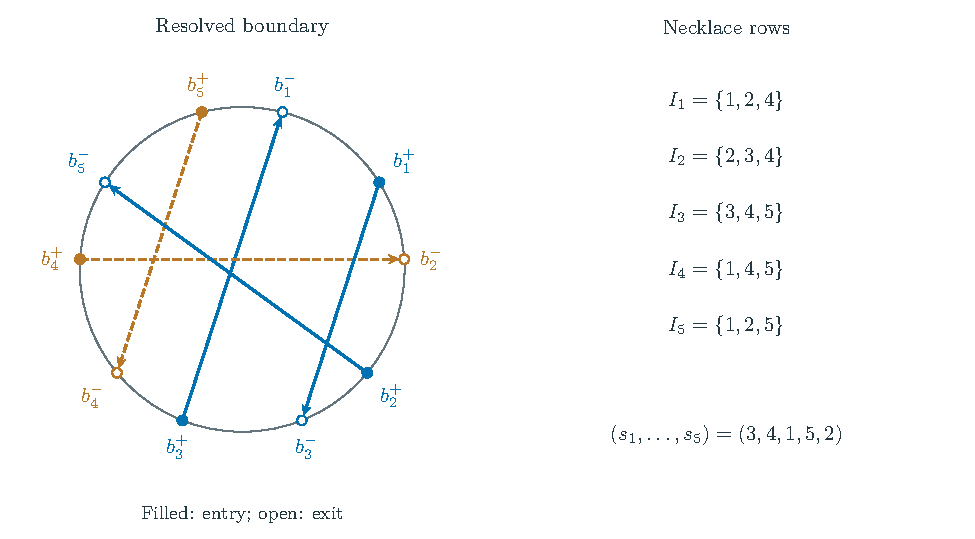
\includegraphics[width=\linewidth]{figures/clh_boundary_necklace.pdf}
\caption{The resolved boundary and necklace of $f=(3,5,6,7,9)$. Chords point from entry to exit; their intersections depict endpoint interlacing. Filled entries and open exits remain distinct when they share an integer label. The necklace rows on the right record membership on the half-open arcs $(s_p,p]$.}
\label{fig:clh-boundary-necklace}
\end{figure}

\paragraph{Pair classes.}
The seven directed crossing edges are
\[
 E_f=\{(1,2),(2,3),(2,4),(3,5),(4,5),(5,1),(5,2)\}.
\]
Exactly $(2,4)$, $(4,5)$ and $(5,2)$ have $s_p=q$.
The remaining unordered pairs are
\[
 \mathrm{Mis}^{\uparrow\downarrow}_f=\{\{1,3\}\},\qquad
 \mathrm{Mis}^{\downarrow\uparrow}_f=\{\{1,4\}\},\qquad
 \text{alignment: }\{3,4\}.
\]
No necklace row contains both $1$ and $3$, and every row contains $1$ or $4$.
Thus both misalignment columns vanish; the alignment is absent from the exponent formula.
Figure~\ref{fig:clh-pair-classes} shows one representative of each class.

\clearpage
\paragraph{Matrices.}
Number the crossing columns in the displayed order of $E_f$, from $1$ to $7$.
Figure~\ref{fig:clh-matrix-worked} gives $M_N$, $P_fDM_N$ and $B$ in that order.
The three other unordered-pair columns are zero in all three matrices and are omitted from the display.
For example, column $2$, the edge $2\to3$, reads
\[
 m=(-1,0,0,0,-1)^{\mathsf T},\qquad
 P_fDm=(0,-1,1,0,0)^{\mathsf T}=e_3-e_2.
\]

\begin{figure}[htbp]
\centering
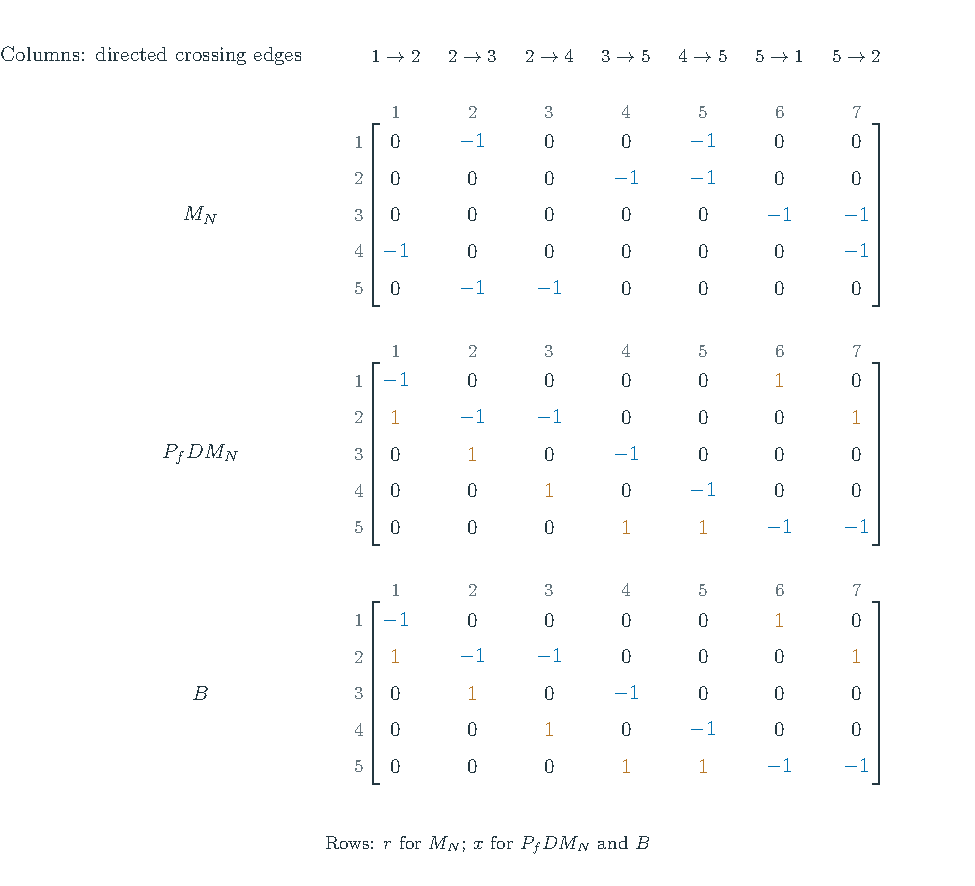
\includegraphics[width=\linewidth]{figures/clh_matrix_worked.pdf}
\caption{The seven crossing columns for $f=(3,5,6,7,9)$, in the order shown above the matrices. Necklace positions index the rows of $M_N$; exit labels index the rows of $P_fDM_N$ and $B$. The two lower matrices agree entry by entry. All three omitted noncrossing columns are zero.}
\label{fig:clh-matrix-worked}
\end{figure}

Figure~\ref{fig:clh-lean-column} follows two columns of Figure~\ref{fig:clh-matrix-worked} through $D$ and $P_f$.

\begin{figure}[htbp]
\centering
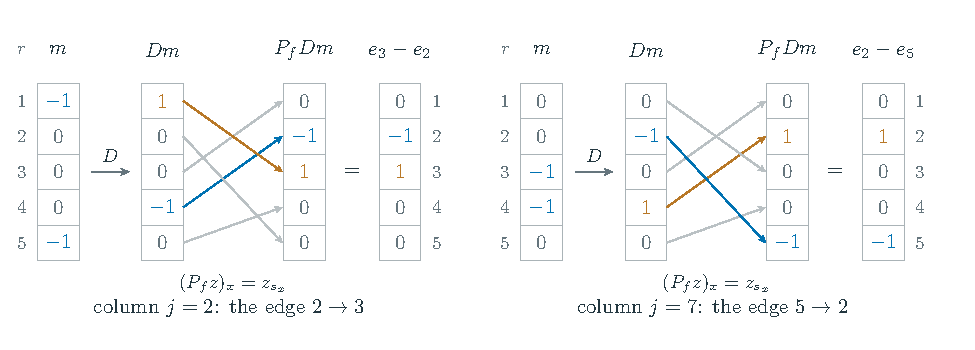
\includegraphics[width=\linewidth]{figures/clh_lean_column.pdf}
\caption{Columns $j=2$ (the edge $2\to3$) and $j=7$ (the edge $5\to2$) of Figure~\ref{fig:clh-matrix-worked}, followed from the column $m$ of $M_N$ through $D$ and $P_f$ to the column of $B$, for $\ba=(3,5,1,2,4)$ and $s=(3,4,1,5,2)$. Row $x$ of $P_fDm$ is row $s_x$ of $Dm$; blue marks $-1$ and ochre $+1$. Evaluated by the formal definitions of Appendix~\ref{app:lean-interface}.}
\label{fig:clh-lean-column}
\end{figure}

\clearpage
\paragraph{Half-open columns.}
For a column indexed by $p\to q$, the entry of $M_N$ on row $r$ is
$-\mathbf1_{r\in(s_p,s_q]}$. In column order, the seven arcs are
\[
 (3,4],\ (4,1],\ (4,5],\ (1,2],\ (5,2],\ (2,3],\ (2,4],
\]
and their row sets are, respectively,
\[
 \{4\},\ \{1,5\},\ \{5\},\ \{2\},\ \{1,2\},\ \{3\},\ \{3,4\}.
\]
In particular, the wrapped arc $(4,1]$ contains rows $5$ and $1$, while its initial row $4$ is excluded.
Figure~\ref{fig:clh-column-arcs} draws the seven arcs.

\begin{figure}[htbp]
\centering
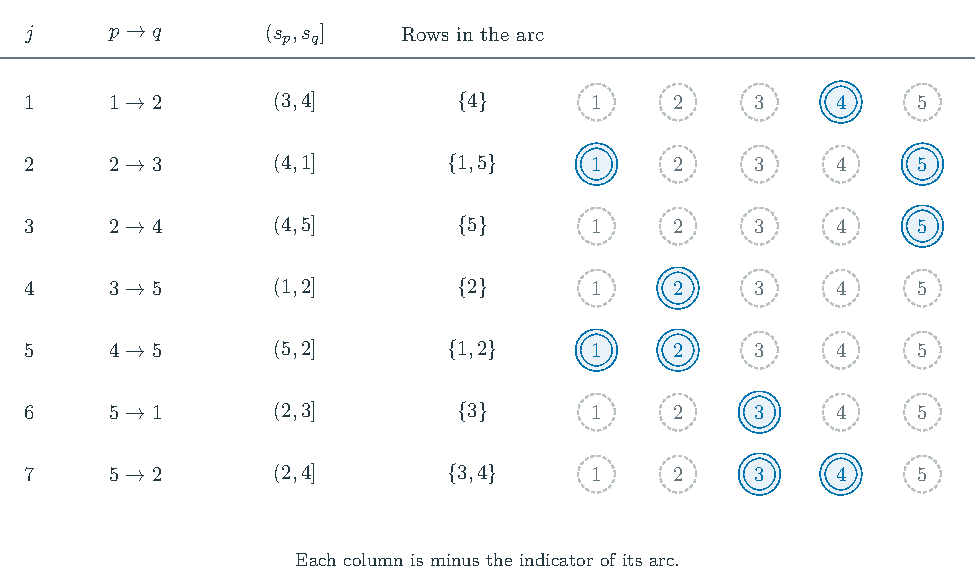
\includegraphics[width=\linewidth]{figures/clh_column_arcs.pdf}
\caption{Every crossing column as a half-open arc of necklace rows. Double solid circles mark rows in the arc; dashed circles mark the other rows. The exponent is $-1$ on the marked rows and $0$ elsewhere. The cyclic order makes $(4,1]=\{5,1\}$ and $(5,2]=\{1,2\}$.}
\label{fig:clh-column-arcs}
\end{figure}

\paragraph{Partitions.}
The two winding-one partitions in Figure~\ref{fig:clh-partitions} are
\[
 \{(1,2,3,5),(2,4,5)\},\qquad
 \{(1,2,4,5),(2,3,5)\}.
\]
Both have two cycles, one containing the wrapped edge $(5,1)$ and the other $(5,2)$.
Each cycle advances a total of $5$ around the labels, so its winding is one.
Either choice therefore gives the cycle decomposition used in the Hessian argument.

\end{document}
